%For printing uncomment below line and comment next line
%\PassOptionsToClass{12pt,a4paper, openright, toc = bibliography}{report}
\PassOptionsToClass{12pt,a4paper, toc = bibliography}{report} 
\documentclass{report}
%For printing uncomment below line
%\usepackage[a4paper, twoside, inner=3cm, outer=3cm, bindingoffset=1cm]{geometry} 
\usepackage{graphicx}
\usepackage{times}
\usepackage{url}
\usepackage[english]{babel}
\usepackage[acronym,nonumberlist,sort=use]{glossaries}
\usepackage{verbatim}
\usepackage{tikz}
\usepackage{circuitikz}
\usepackage{wrapfig}
\usepackage{amsmath}
\usepackage{nomencl}
\usepackage{accents}
\usepackage{amssymb}
\usepackage{minted}
\usepackage{listings}
\usepackage{minted}
\usepackage{caption}
\usepackage{svg}
\usepackage{hyperref}
\usepackage{algorithm2e}
\usepackage{algpseudocode}
\hypersetup{
    colorlinks=true,
    linkcolor=violet,
    filecolor=blue,      
    urlcolor=blue,
    citecolor=blue,
}

\usepackage{miller}

\usepackage{multirow}
\usepackage{multicol}
\usepackage{siunitx}
\usepackage{array}
\usepackage{placeins}
\usepackage{float}
\usepackage{caption}
\usepackage{subcaption}
\usepackage{pdfpages}



\setlength{\parindent}{0pt}

\setlength{\textheight}{245mm}
\setlength{\textwidth}{160mm}

\setlength{\headheight}{3mm}
\setlength{\headsep}{12mm}
\setlength{\topmargin}{15mm}

\setlength{\hoffset}{-10mm} % already accounted for in the margins
\setlength{\voffset}{-30mm} % already accounted for in the margins
% line, paragraphs indent & spacing

\pdfinfo{
   /Author (Achal H P)
   /Title  (MTech Thesis)
   /Subject (CP Modeling of Discrete Twin Evolution in HCP Metals)
}



\begin{document}

\begin{titlepage}
    \centering
    {\huge\bfseries Crystal Plasticity Modeling of Discrete Twin Evolution in Hexagonal Closed Packed Metals\par}
    \vspace{2cm}
    {\large A thesis submitted in partial fulfillment of \\  the requirements for the degree of \par}
    \vspace{0.5cm}
    {\large \bf Master of Technology}\\
    \vspace{0.5cm}
    {\large by }\\
    \vspace{1cm}
    {\large \bf Achal H. P.} \\
    {\large \bf (Roll No. ME22MT011)} \\
    \vspace{1.5cm}
    {\large Under the Supervision of} \\
    {\large \bf Professor Satyapriya Gupta \par}
    \vfill
    
\includegraphics[width=6.5cm]{images/IIT Dh Logo.png}\\[\baselineskip]
    \vfill
    {\large \uppercase{Department of Mechanical, Materials, \\ and Aerospace Engineering}\par}
    \vspace{0.25cm}
    {\scshape\LARGE indian institute of technology dharwad\par}
    \vspace{0.5cm}
    {\large May 2024}
\end{titlepage}

\pagenumbering{roman}

\newpage
\cleardoublepage
\thispagestyle{empty}
\begin{center}
    \vspace*{\stretch{1}}
    {Dedicated to my grandmothers Subbalakshmi and Devakiamma.\par}
    \vspace{1cm}
    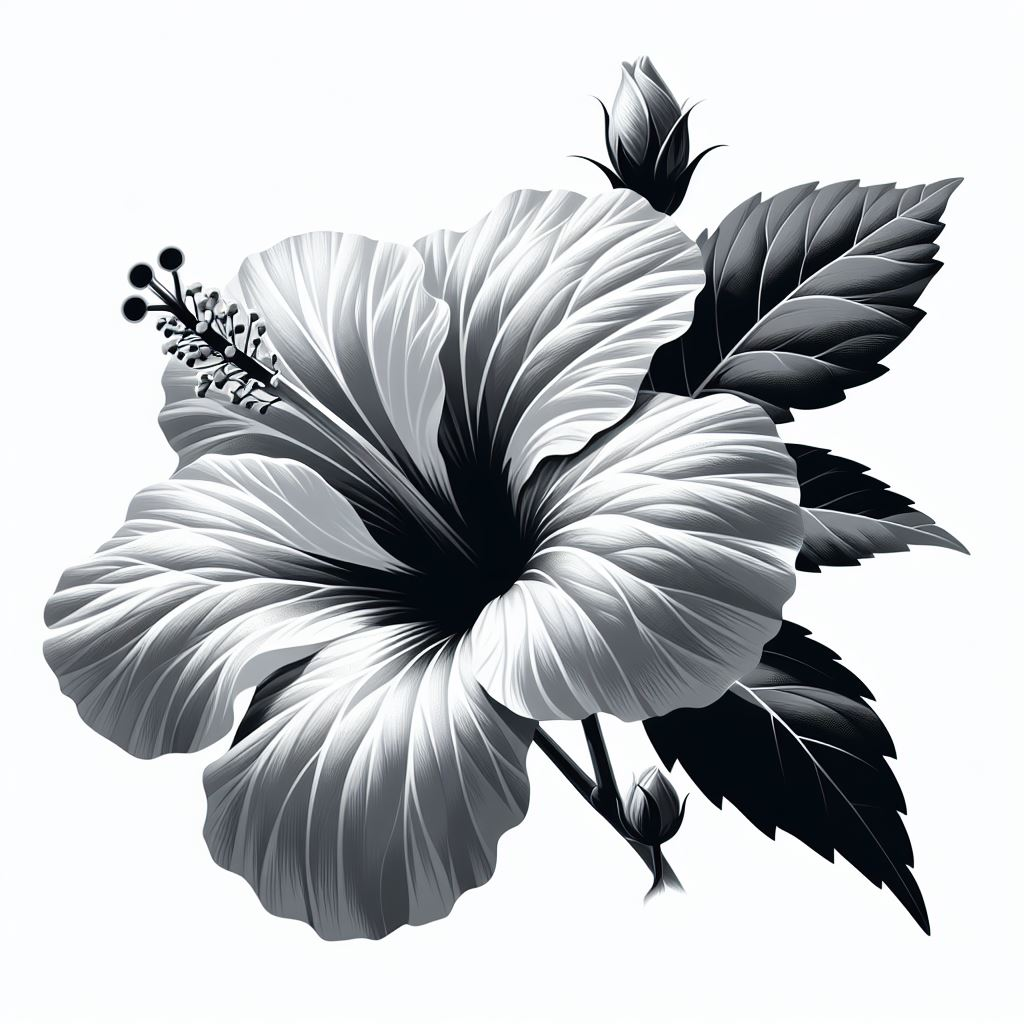
\includegraphics[width=3cm]{images/Hibiscus.png}
    \vspace*{\stretch{1}}
\end{center}

\chapter*{\centering Acknowledgements}
  {\fontsize{14}{16}\selectfont I would like to thank my supervisor Prof. Satyapriya Gupta for his guidance throughout the project. I would also like to thank the EICMD team for their guidance, SERB for providing SRG grant which equipped us with computational hardware and IIT Dharwad for providing facilities and conductive environment.}

\newpage
\cleardoublepage
\thispagestyle{empty}
\begin{center}
    {\LARGE \bf Thesis Approval}\\
    \vspace{1.5cm}
    {\large The thesis entitled}\\
    {\huge\bfseries Crystal Plasticity Modeling of Discrete Twin Evolution in Hexagonal Closed Packed Metals\par}
    \vspace{0.4cm}
    {\large by}\\
    \vspace{0.4cm}
    {\Large \bf Achal H. P.}\\
    \vspace{2mm}
    {\large (Roll No. ME22MT011)}\\
    \vspace{0.3cm}
    {\large is approved for the degree of}\\
    \vspace{0.5cm}
    {\Large \bf Master of Technology}\\
    \vspace{0.3cm}
    {\large from the}\\
    \vspace{0.3cm}
    {\Large \bf Indian Institute of Technology Dharwad}\\
    \vspace{2cm}
    \begin{tabular}{ccc}
      \rule{6.5cm}{1sp}                &\rule{10mm}{0pt}& \rule{6.5cm}{1sp} \\ \vspace{-0.4cm} \\
      {\Large \textbf{Prof. Somashekara M. A.}}                 && {\Large \textbf{Prof. Amlan Barua}} \\ \vspace{-0.2cm} \\
      {\large Chairperson}     && {\large External Examiner} \\ \vspace{1.5cm} \\
      \rule{6.5cm}{1sp}                && \rule{6.5cm}{1sp} \\ \vspace{-0.4cm} \\
      {\Large \textbf{Prof. Tejas P. Gotkhindi}}           && {\Large \textbf{Prof. Satyapriya Gupta}} \\  \vspace{-0.2cm} \\
      {\large Internal Examiner}    && {\large Supervisor} \\ \vspace{2cm} \\
    \end{tabular}
    {\raggedright \Large  Date: 20 May 2024} \\ \vspace{0.5cm}
    {\Large  Place: Dharwad} 
\end{center}

\chapter*{\centering Declaration}
  {\fontsize{14}{16}\selectfont   
  I declare that the thesis entitled ``Crystal Plasticity Modeling of Discrete Twin Evolution in Hexagonal Closed Packed Metals" submitted by me for the degree of Master of Technology (MTech.) is a bonafide record of research carried out by me under the supervision of Dr. Satyapriya Gupta. The content of this thesis, in full or in parts, have not been submitted to any other Institute or University for the award of any Degree or Diploma.}

  \vskip 2cm 

  \begin{tabular}{p{5cm} p{4cm} c}
    & & \rule{6cm}{1sp} \\
    {\fontsize{14}{16}\selectfont Dharwad}& & {\fontsize{14}{16}\selectfont Achal H. P.} \\
    {\fontsize{14}{16}\selectfont Date: 20 May 2024} & & {\fontsize{14}{16}\selectfont Roll No. ME22MT011} \\
  \end{tabular}
%\rule{3cm}{1sp}


\chapter*{\centering Abstract}
  {\fontsize{14}{16}\selectfont Hexagonal close-packed (HCP) metals and alloys exhibit a remarkable array of distinct properties, rendering them invaluable across numerous industrial sectors, including nuclear, aerospace, automotive, and bioengineering applications. The development of accurate modeling for the deformation behavior of these materials is imperative for cost-effective fabrication techniques.

Deformation twinning represents a crucial contributor to the plastic deformation of HCP metals and alloys. The modeling of deformation twinning along with dislocation-mediated plasticity has been a challenging task. Widely used phenomenological models\footnote{S. R. Kalidindi, “Incorporation of deformation twinning in crystal plasticity models,” Journal of the Mechanics and Physics of Solids, vol. 46, no. 2, pp. 267–290, 1998} for deformation twinning omit the stochastic nature of twinning for the sake of simplicity. Additionally, most models employ the volume fraction method, which is non-physical \footnote{Y. Paudel, D. Giri, M. W. Priddy, C. D. Barrett, K. Inal, M. A. Tschopp, H. Rhee, and H. El Kadiri, “A review on capturing twin nucleation in crystal plasticity for hexagonal metals,” Metals, vol. 11, no. 9, 2021. }, treating twinning as a diffuse or continuous quantity. This approach fails to capture the intricate twin morphology within the Representative Volume Element. Recent models aimed at accurate prediction of twin formation utilize energy-based or phase-field techniques, which are computationally expensive.

The aim of this project is the development of a "discrete twin model" that is computationally efficient yet accurately predicts twin formation. The primary objective is the improvement of the existing phenomenological model by incorporating the stochastic nature of twin formation and growth, and modeling the physically accurate spatial resolution of twin morphology as a discrete entity. This approach is expected to lead to accurate prediction of texture evolution during plastic deformation. The secondary objective is the modeling of the sudden "jump" of shear and reorientation caused by twin formation in the kinematics of the constitutive law.

The proposed "discrete twin model" accomplishes to model the stochastic nature of twinning using a random sampling technique inspired by the Monte Carlo method, while the spatial resolution of texture evolution is accomplished by modeling twinning as a discrete entity. The insights gained from this project are anticipated to contribute to the development of improved constitutive models for studying the plastic deformation behavior of HCP metals.}

\tableofcontents

%\chapter*{Nomenclature}
%\addcontentsline{toc}{chapter}{Nomenclature}

\listoffigures
\addcontentsline{toc}{chapter}{List of figures}

\listoftables
\addcontentsline{toc}{chapter}{List of tables}

%\chapter*{List of Symbols}
%\addcontentsline{toc}{chapter}{List of Symbols}


\chapter{Introduction}
\pagenumbering{arabic}
\section{Motivation}
Hexagonal close-packed (HCP) metals and alloys exhibit a remarkable array of distinct properties, rendering them invaluable across numerous industrial sectors, including nuclear, aerospace, automotive, and bioengineering applications. However, the inherent anisotropic nature arising from their non-symmetric hexagonal crystal lattice significantly influences their deformation behavior, making the fabrication of components from these metals an intricate and costly endeavor. To mitigate manufacturing expenses and to foster more widespread adoption of HCP metals and alloys, developing a comprehensive understanding enabling the accurate modeling of their deformation behavior is imperative.

\vspace{3mm}
Deformation/Mechanical twinning is one of the important contributor in the plastic deformation of HCP metals and alloys. Modeling deformation twinning along with the dislocaton mediated plasticity has been a challenging task. 

\vspace{3mm}
Most models use volume fraction method which is nonphysical \cite{Paduel202111091373}. This approach treats twinning as a diffuse quantity while in reality twinning manifests as a discrete entity. Furthermore, this approach fails to capture the intricate twin morphology within the Representative Volume Element. 

\vspace{3mm}
In the case of deformation kinematics, upon formation, a deformation twin induces a sudden change in shear and it reorients the lattice. Incorporating this sudden transformation needs a distinct approach to handling the kinematics within the constitutive model.

\vspace{3mm}
Many widely used phenomenological models\cite{KALIDINDI1998267} for deformation twinning also omit the stochastic nature of twinning for simplicity. Recent models which use energy based or phase field techniques to model twinning are computationally expensive.

\section{Research Objectives}
The primary objectives of the proposed ``discrete twinning model" are as follows:
\begin{enumerate}
    \item To be computationally efficient yet accurately predict the twin formation.
    \item To model the stochastic nature of twinning.
    \item To capture the physically accurate spatial resolution of a twin which is a discrete entity. 
    \item To capture the morphology of twin nucleation and growth.
    \item To apply the ``sudden" reorientation and shear caused by the twinning at a appropriate timescale in the kinematics of the constitutive law. 
\end{enumerate}

\section{Outline of the thesis}
\begin{itemize}
    \item This chapter contains details about thesis organization and brief introduction to the topic.
    \item Second chapter contains literature review.
    \item Third chapter contains development of new constitutive model for deformation twinning.
    \item Fourth chapter contains model testing.
    \item Fifth chapter contains conclusions and future scope.
\end{itemize}

\section{Brief introduction to the topics}

\subsection{HCP Metals}
The Hexagonal Close Packed (HCP) structure is a densely packed arrangement of equal spheres in a regular, infinite lattice. The HCP unit cell can be envisaged as a hexagonal prism, with an atom at each vertex and three additional atoms at the centre. Alternatively, it can be conceptualised as a stack of three closely packed hexagonal layers(ABA), where the top and bottom layers align.
\begin{figure}[H]
  \centering
  \includesvg[width=3cm]{images/Hexagonal_close_packed.svg}
  \caption{Unit cell structure of HCP [Wikipedia image]}
\end{figure}

Magnesium, Titanium, Zirconium and Beryllium are the most commonly used HCP metals in structural applications, with Hexagonal Close Packed lattice.

\vspace{3mm}
Magnesium and Titanium are known for their excellent \textbf{strength-to-weight ratio} and fatigue resistance, making them ideal for use in various sectors such as automotive, aviation, defence, and spacecraft applications\cite{app11156861}. 

\vspace{3mm}
Titanium and Zirconium, due to their good \textbf{corrosion resistance}, find applications in high-temperature environments like gas turbines and nuclear reactors.

\vspace{3mm}
Beryllium, characterised by its \textbf{low thermal expansion coefficient}, high stiffness, and high strength-to-weight ratio, is used in spacecraft components \cite{Feinberg10.1117/12.924271}. Beryllium is also used as x-ray tubes and lenses, because it is transparent to x-rays and strong enough to hold vacuum \cite{rogers1947high}.

\vspace{3mm}
Titanium and Magnesium, due to their \textbf{compatibility with biological tissues}, are utilised in biomedical applications.

\vspace{3mm}
Beryllium and Zirconium, owing to their very \textbf{low neutron absorption cross-section}, are widely used in the construction of structural components inside a nuclear reactor\cite{Tomberlin_osti_910826}.

\begin{figure}[H]
  \centering
  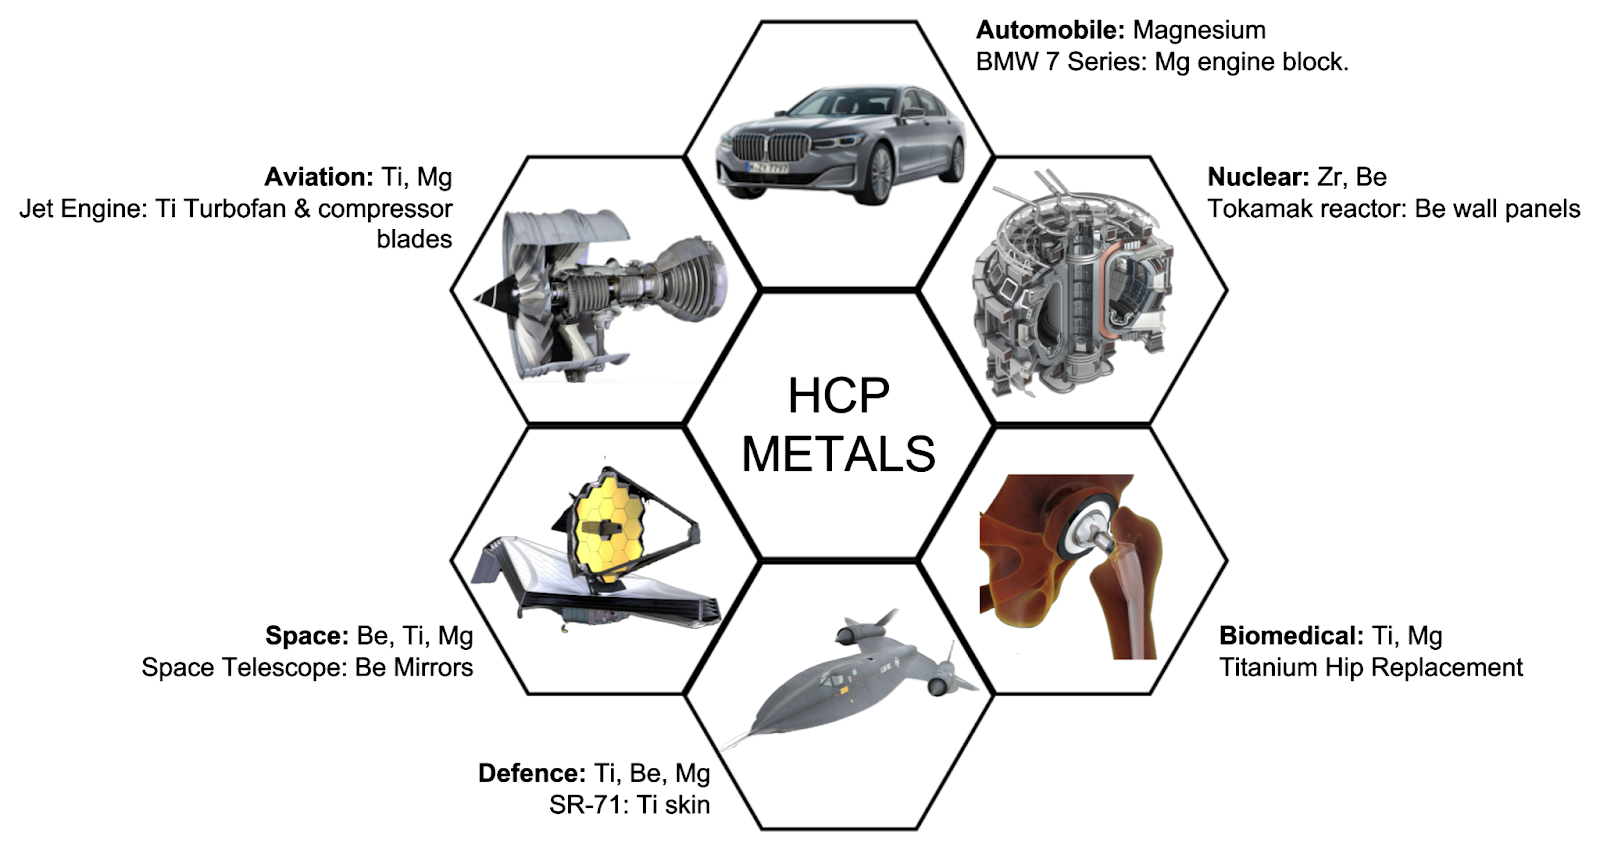
\includegraphics[width=\textwidth]{images/HCP_metals.png}
  \caption{Application of HCP metals in different industrial sectors}
\end{figure}

\vspace{3mm}
However, the widespread use of HCP metals is limited due to the challenges in fabrication, primarily because of their complex deformation behaviour and low ductility. The objective of our study is to gain a deeper understanding of the intricate deformation behaviour of HCP metals, which could potentially enhance manufacturing processes.

\subsection{Twinning}

\begin{figure}[H]
  \centering
  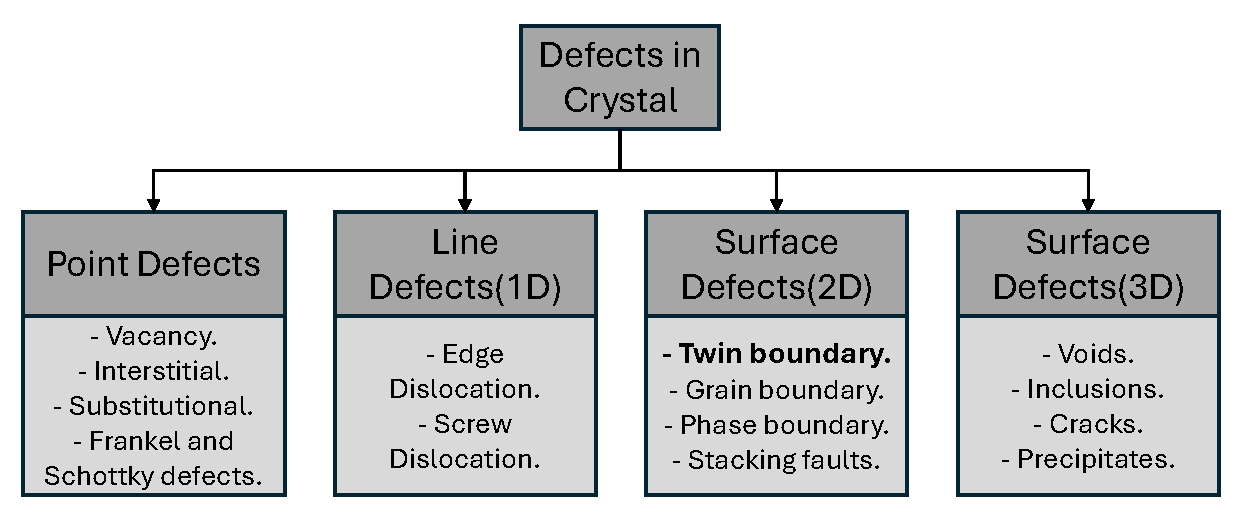
\includegraphics[width=0.8\textwidth]{images/Defects_in_crystals.pdf}
  \caption{Defects in Crystalline Materials.}
  \label{CrystalDefects}
\end{figure}



Twinning is a 2D defect which is characterized by a special form of grain boundary called twin boundary. Twin boundary separates two crystals and at the plane of twin boundary the lattice of two crystals appears to be mirrored as shown in figure \ref{fig:Twinning in 2D}.

\begin{figure}[H]
    \centering
    \resizebox{0.4\textwidth}{!}{
    \begin{circuitikz}
\tikzstyle{every node}=[font=\LARGE]
\draw [short] (11.5,23) -- (2.5,23) ;
\draw [ fill={rgb,255:red,0; green,17; blue,250} ] (2.75,25.25) circle (0.25cm);
\draw [ fill={rgb,255:red,0; green,17; blue,250} ] (5.5,25.25) circle (0.25cm);
\draw [ fill={rgb,255:red,29; green,250; blue,0} ] (4.5,22.25) circle (0.25cm);
\draw [ fill={rgb,255:red,0; green,17; blue,250} ] (3.75,24.5) circle (0.25cm);
\draw [ fill={rgb,255:red,0; green,17; blue,250} ] (5,24.5) circle (0.25cm);
\draw [ fill={rgb,255:red,29; green,250; blue,0} ] (5.25,23) circle (0.25cm);
\draw [ fill={rgb,255:red,0; green,17; blue,250} ] (4.25,25.25) circle (0.25cm);
\draw [ fill={rgb,255:red,0; green,17; blue,250} ] (6.75,25.25) circle (0.25cm);
\draw [ fill={rgb,255:red,0; green,17; blue,250} ] (6.25,24.5) circle (0.25cm);
\draw [ fill={rgb,255:red,0; green,17; blue,250} ] (8,25.25) circle (0.25cm);
\draw [ fill={rgb,255:red,0; green,17; blue,250} ] (4.5,23.75) circle (0.25cm);
\draw [ fill={rgb,255:red,0; green,17; blue,250} ] (10,24.5) circle (0.25cm);
\draw [ fill={rgb,255:red,0; green,17; blue,250} ] (7.5,24.5) circle (0.25cm);
\draw [ fill={rgb,255:red,0; green,17; blue,250} ] (9.25,25.25) circle (0.25cm);
\draw [ fill={rgb,255:red,0; green,17; blue,250} ] (5.75,23.75) circle (0.25cm);
\draw [ fill={rgb,255:red,0; green,17; blue,250} ] (7,23.75) circle (0.25cm);
\draw [ fill={rgb,255:red,0; green,17; blue,250} ] (8.25,23.75) circle (0.25cm);
\draw [ fill={rgb,255:red,0; green,17; blue,250} ] (8.75,24.5) circle (0.25cm);
\draw [ fill={rgb,255:red,0; green,17; blue,250} ] (9.5,23.75) circle (0.25cm);
\draw [ fill={rgb,255:red,0; green,17; blue,250} ] (10.75,23.75) circle (0.25cm);
\draw [ fill={rgb,255:red,29; green,250; blue,0} ] (6.5,23) circle (0.25cm);
\draw [ fill={rgb,255:red,29; green,250; blue,0} ] (7.75,23) circle (0.25cm);
\draw [ fill={rgb,255:red,29; green,250; blue,0} ] (9,23) circle (0.25cm);
\draw [ fill={rgb,255:red,29; green,250; blue,0} ] (10.25,23) circle (0.25cm);
\draw [ fill={rgb,255:red,29; green,250; blue,0} ] (11.5,23) circle (0.25cm);
\draw [ fill={rgb,255:red,29; green,250; blue,0} ] (3.75,21.5) circle (0.25cm);
\draw [short] (11.5,20.75) -- (2.75,20.75);
\draw [ fill={rgb,255:red,29; green,250; blue,0} ] (2.75,20.75) circle (0.25cm);
\draw [ fill={rgb,255:red,29; green,250; blue,0} ] (5.75,22.25) circle (0.25cm);
\draw [ fill={rgb,255:red,29; green,250; blue,0} ] (7,22.25) circle (0.25cm);
\draw [ fill={rgb,255:red,29; green,250; blue,0} ] (8.25,22.25) circle (0.25cm);
\draw [ fill={rgb,255:red,29; green,250; blue,0} ] (9.5,22.25) circle (0.25cm);
\draw [ fill={rgb,255:red,29; green,250; blue,0} ] (10.75,22.25) circle (0.25cm);
\draw [ fill={rgb,255:red,29; green,250; blue,0} ] (5,21.5) circle (0.25cm);
\draw [ fill={rgb,255:red,29; green,250; blue,0} ] (6.25,21.5) circle (0.25cm);
\draw [ fill={rgb,255:red,29; green,250; blue,0} ] (7.5,21.5) circle (0.25cm);
\draw [ fill={rgb,255:red,29; green,250; blue,0} ] (8.75,21.5) circle (0.25cm);
\draw [ fill={rgb,255:red,29; green,250; blue,0} ] (10,21.5) circle (0.25cm);
\draw [ fill={rgb,255:red,29; green,250; blue,0} ] (4.25,20.75) circle (0.25cm);
\draw [ fill={rgb,255:red,29; green,250; blue,0} ] (5.5,20.75) circle (0.25cm);
\draw [ fill={rgb,255:red,29; green,250; blue,0} ] (6.75,20.75) circle (0.25cm);
\draw [ fill={rgb,255:red,29; green,250; blue,0} ] (8,20.75) circle (0.25cm);
\draw [ fill={rgb,255:red,29; green,250; blue,0} ] (9.25,20.75) circle (0.25cm);
\draw [ fill={rgb,255:red,0; green,17; blue,250} ] (3.5,20) circle (0.25cm);
\draw [ fill={rgb,255:red,0; green,17; blue,250} ] (5,20) circle (0.25cm);
\draw [ fill={rgb,255:red,0; green,17; blue,250} ] (6.25,20) circle (0.25cm);
\draw [ fill={rgb,255:red,0; green,17; blue,250} ] (7.5,20) circle (0.25cm);
\draw [ fill={rgb,255:red,0; green,17; blue,250} ] (8.75,20) circle (0.25cm);
\draw [ fill={rgb,255:red,0; green,17; blue,250} ] (10,20) circle (0.25cm);
\draw [ fill={rgb,255:red,0; green,17; blue,250} ] (4.25,19.25) circle (0.25cm);
\draw [ fill={rgb,255:red,0; green,17; blue,250} ] (5.75,19.25) circle (0.25cm);
\draw [ fill={rgb,255:red,0; green,17; blue,250} ] (7,19.25) circle (0.25cm);
\draw [ fill={rgb,255:red,0; green,17; blue,250} ] (8.25,19.25) circle (0.25cm);
\draw [ fill={rgb,255:red,0; green,17; blue,250} ] (9.5,19.25) circle (0.25cm);
\draw [ fill={rgb,255:red,0; green,17; blue,250} ] (10.75,19.25) circle (0.25cm);
\draw [ fill={rgb,255:red,0; green,17; blue,250} ] (5.25,18.5) circle (0.25cm);
\draw [ fill={rgb,255:red,0; green,17; blue,250} ] (6.5,18.5) circle (0.25cm);
\draw [ fill={rgb,255:red,0; green,17; blue,250} ] (7.75,18.5) circle (0.25cm);
\draw [ fill={rgb,255:red,0; green,17; blue,250} ] (9,18.5) circle (0.25cm);
\draw [ fill={rgb,255:red,0; green,17; blue,250} ] (10.25,18.5) circle (0.25cm);
\draw [ fill={rgb,255:red,0; green,17; blue,250} ] (11.5,18.5) circle (0.25cm);
\node [font=\large] at (13.5,23) {Twin Boundary};
\node [font=\large] at (13.5,20.75) {Twin Boundary};
\end{circuitikz}
}
    \caption{Twinning illustrated in 2D}
    \label{fig:Twinning in 2D}
\end{figure}

Twinning can be caused by different mechanisms. The twins are:
\begin{itemize}
    \item Growth twins.
    \item Transformation twins.
    \item Deformation twins.
\end{itemize}

\subsubsection{Deformation twinning}

Deformation twinning allows a mode of plastic deformation in crystalline structures. Deformation twinning occurs if one layer of crystals changes its orientation under shear stress.

``A deformation twin is a region of a crystalline body which had undergone a homogeneous shape deformation in such a way that the resulting
product structure is identical with that of the parent, but oriented differently." Bilby and Crocker \cite{doi:10.1098/rspa.1965.0216}

If the shear angle is known it is possible to measure the deformation caused by the twinning. We use this information for into our constitutive model.


\subsection{Deformation mechanisms in HCP metals.}
Slip and deformation twinning are major deformation modes which mediate plastic deformation in HCP metals. 
Five families of slip systems have been identified and they are given in the Table \ref{Slip_systems} \cite{Partridge1967TheCA}.

\begin{table}[H]
\centering
\caption{Number of total and independent slip systems.}
\renewcommand\arraystretch{1.2}
\renewcommand\baselinestretch{1.2}
\begin{tabular}{|c|c|c|c|}
\hline
\multirow{2}{5em}{Slip system family} & \multirow{2}{3em}{Burgers vector} & \multicolumn{2}{c|}{No. of slip systems} \\
\cline{3-4}
 & & Total & Independent \\
 \hline
 $\langle11\Bar{2}0\rangle\{0001\}$ & $\langle a \rangle$ & 3 & 2 \\
 $\langle11\Bar{2}0\rangle\{1\Bar{1}00\}$ & $\langle a \rangle$ & 3 & 2 \\
 $\langle11\Bar{2}0\rangle\{10\Bar{1}1\}$ & $\langle a \rangle$ & 6 & 4 \\
 $\langle11\Bar{2}3\rangle\{10\Bar{1}1\}$ & $\langle c+a \rangle$ & 6 & 5 \\
 $\langle11\Bar{2}3\rangle\{11\Bar{2}2\}$ & $\langle c+a \rangle$ & 6 & 5 \\
 \hline
\end{tabular}

\label{Slip_systems}
\end{table}

Figure \ref{HCP_Slip_Twin_Systems} gives representation of most commonly observed slip and tiwn system among all the discussed slip and twin systems in HCP metals.
\begin{figure}[H]
    \centering
    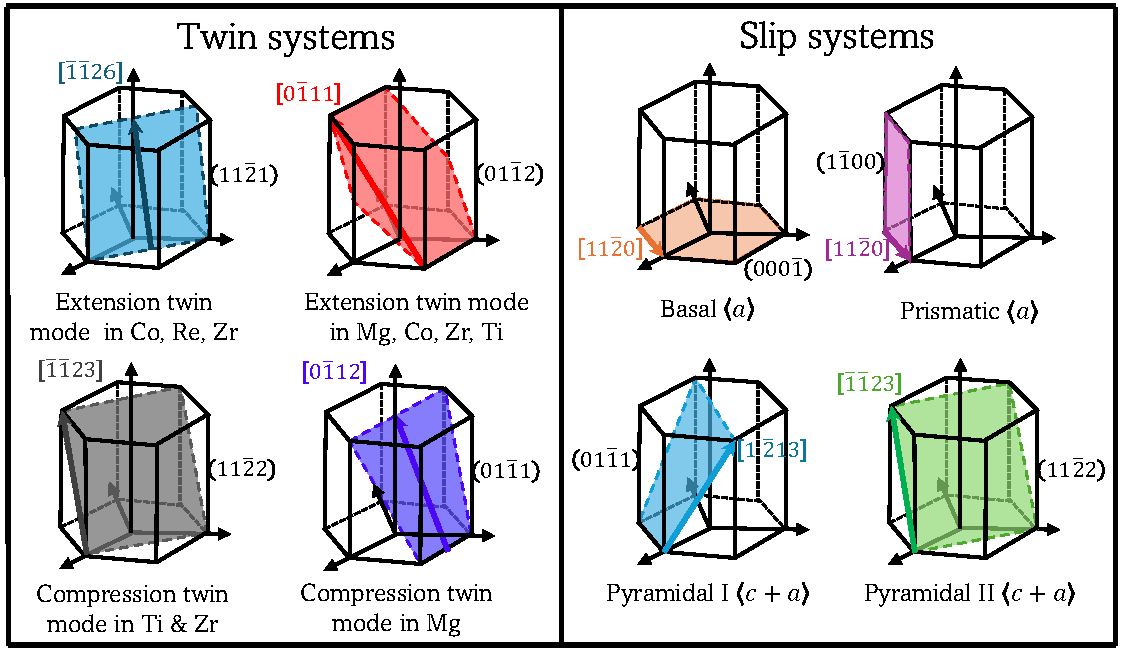
\includegraphics[width=\textwidth]{images/Slip_and_twin_systems.pdf}
    \caption{Commonly observed slip and twin Systems in HCP metals.}
    \label{HCP_Slip_Twin_Systems}
\end{figure}

The first 3 families operate in basal plane and provide only 4 independent slip systems and it is necessary to activate one of $\langle c+a \rangle$ slip systems or twin systems to meet the von Mises criterion \cite{taylor1938plastic} for arbitrary deformation. 

A twin mode or twin system can be described by four elements: undistorted plane $K_1$, the direction of shear $\eta_1$ and second undistorted plane $K_2$ and direction $\eta_2$. Since these 4 elements are interdependent, a twinning mode can be uniquely specified by either $K_1$ and $\eta_1$ or $K_2$ and $\eta_2$. Table \ref{Twin_systems} gives common twinning modes observed in various HCP metals. More details about twinning crystallography is presented in Chapter \ref{sec:twinning_crystallography}.

\begin{table}[H]
\centering
\caption{Commonly observed twinning modes in HCP metals.}
\renewcommand\arraystretch{1.2}
\renewcommand\baselinestretch{1.2}
\begin{tabular}{|c|c|c|c|}
\hline

$k_1$ plane & $\eta_1$ direction & Material \\
 \hline
 $\{10\Bar{1}2\}$ & $\langle 10\Bar{1}\Bar{1} \rangle$ & Cd, Zn, Co, Mg, Zr, Ti, Be  \\
 $\{10\Bar{1}1\}$ & $\langle 10\Bar{1}\Bar{2} \rangle$ & Mg, Ti  \\
 $\{11\Bar{2}2\}$ & $\frac{1}{3} \langle 11\Bar{2}\Bar{3} \rangle$ & Ti, Zr  \\
 $\{11\Bar{2}1\}$ & $\frac{1}{3}\langle \Bar{1}\Bar{1}2 6\rangle$ & Co, Re, Zr, Ti \\
 \hline
\end{tabular}

\label{Twin_systems}
\end{table}



\subsection{Computational Material Science}

The principle behind computational material science is that microstructural parameters determines the functional parameters. If we control the microstructure of the material we can improve the performance or properties of the materials. Figure \ref{Computational_materials} shows the schematic representation of the workflow in the computational material science.

\begin{figure}[H]
    \centering
    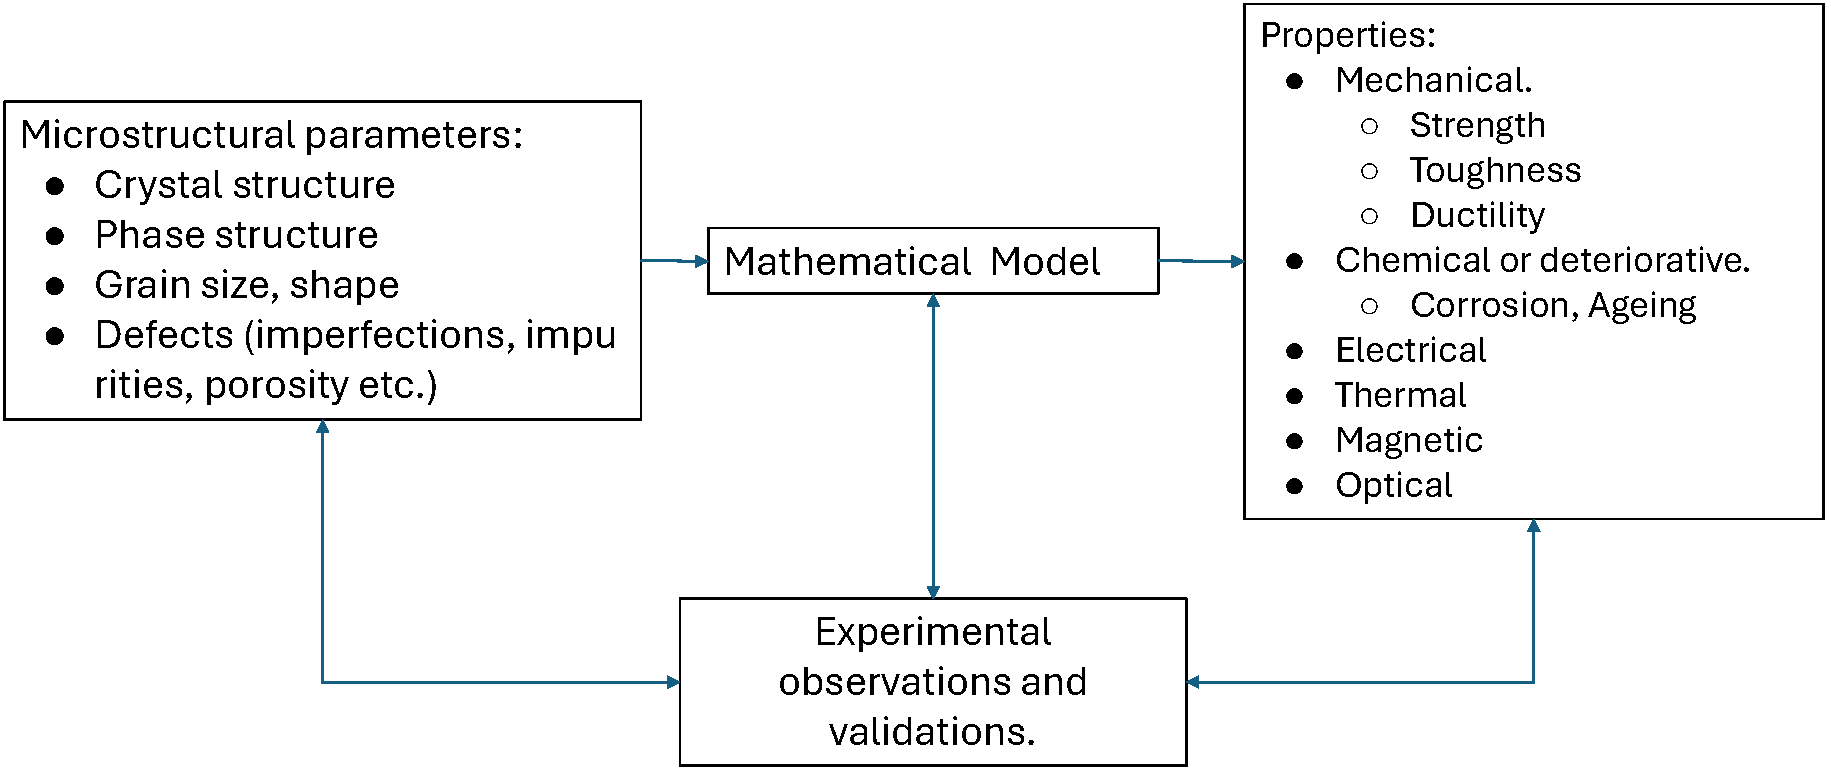
\includegraphics[width=\textwidth]{images/Computational_materials.pdf}
    \caption{Computational Material Science.}
    \label{Computational_materials}
\end{figure}

Computational material science uses the information from the experiments to observe and quantify the microstructural parameters and also to test the performance parameters of the materials. Table
\ref{Microstructural_parameter_exp_technique} adapted from Roters \cite{roters2011advanced} lists the experimental techniques that are used to measure microstructural parameters. 

At the heart of the computational material science is the mathematical model which is used to establish relationship between the microstructural parameters and defects to the performance parameters which are useful for engineering applications of the materials.

The \textbf{crystal plasticity} is the constitutive mathematical model which establishes relationship between the defects like dislocations and twinning with the mechanical properties like strength, ductility, toughness etc. 

\begin{table}[H]
\centering
\caption{Measurable quantities which can be predicted by CPFE models.}
\renewcommand\arraystretch{1.2}
\renewcommand\baselinestretch{1.2}
\begin{tabular}{|c|m{10cm}|}
\hline

  \textbf{Microstructural quantity} & \textbf{Experimental techniques/observations} \\
  \hline
  Dislocation dynamics & Flow stress measurement, transmission electron microscopy, lattice orientation measurements, electron channeling contrast imaging in the scanning electron microscope.  \\
  \hline
  Deformation twinning & Metallography, X-ray and synchrotron diffraction, electron backscatter diffraction, transmission electron microscopy, electron channeling contrast imaging in the scanning electron microscope. \\
  \hline
  Texture evolution & Texture measurements using electron diffraction in the transmission and scanning electron microscope(Kikuchi, SAD, CBED) or X-ray Bragg diffraction.  \\
  \hline
  Crystal Plasticity & Hardness testing, metallography, electrical resistivity, X-ray and synchrotron diffraction, electron backscatter diffraction, transmission electron microscopy, grain size determination, kernel average orientation determination, calorimetry.  \\

 \hline
\end{tabular}

\label{Microstructural_parameter_exp_technique}
\end{table}



\subsubsection{Crystal Plasticity}

\begin{wrapfigure}{rH}{0.45\textwidth}
    \centering 
    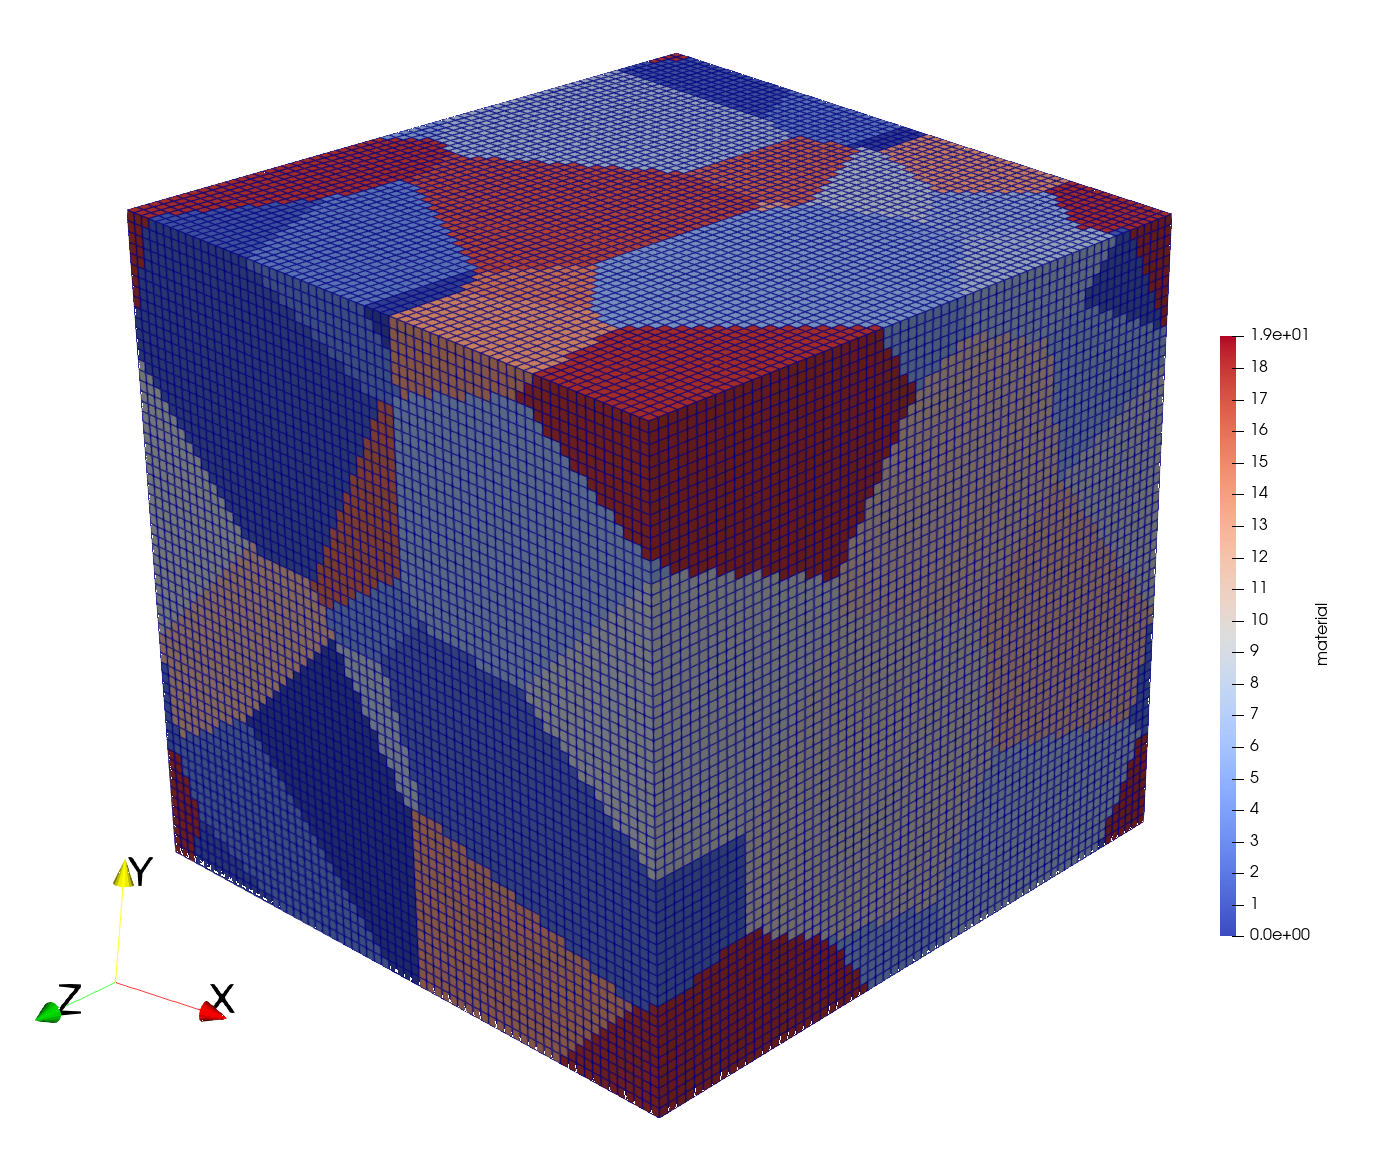
\includegraphics[width=0.4\textwidth]{images/RVE.png}
    \caption{A representative volume element with 20 grains.}
    \label{RVE}
\end{wrapfigure}

Crystal plasticity model is a constitutive mathematical model used to study deformation behavior of materials which are subjected to loads. It mainly contains 3 parts \cite{roters2011advanced}:

\begin{enumerate}
    \item Microstructure parameterization: We choose parameters in the microstructure which may affect the deformation behavior. Lattice parameters, isotropic/non-isotropic, Schmid factor, dislocation density etc.
    \item Laws for Microstructure Evolution Rates: Hardening laws, isotropic or kinematic, slip resistance, interaction matrix etc.
    \item Deformation kinetics: This is the part which connects the evolution of defects to the plastic deformation behavior by evaluating plastic deformation gradient.
\end{enumerate}

The crystal plasticity simulation is often done on a ``Representative Volume Element" which is a numerical representation of a polycrystal. An example RVE is shown in the figure \ref{RVE}



\vspace{2mm}
\textbf{Crystal Plasticity FEM/FFT:}

Most of the crystal plasticity models are formulated in the framework of continuum mechanics which is discussed in Appendix \ref{Appendix:Continuum_mechanics}. Figure below is the schematic of crystal plasticity in framework of continuum mechanics.

\begin{figure}[H]
    \centering
    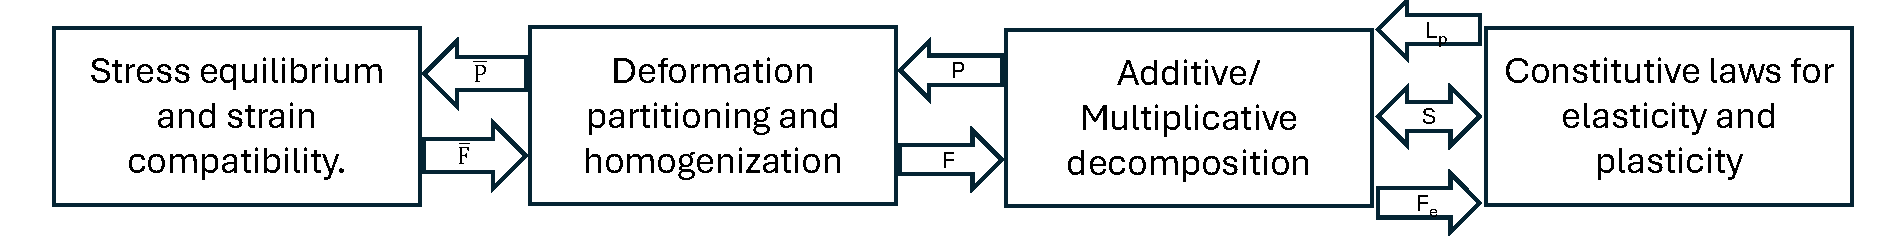
\includegraphics[width=\textwidth]{images/Typical_Crystal_Plasticity_model.pdf}
    \caption{A typical Crystal Plasticity scheme.}
    \label{Typical_CP_model}
\end{figure}

\textbf{Solution methodology:}

Solution methodology involves solving partial differential equations (PDEs) which describes the stress equilibrium. Most commonly used technique to solve the PDEs is ``Finite Element Method". If the boundary conditions are periodic and geometry is simple, solving the partial differential equations can be done using a faster alternative method ``Fast Fourier Transform(FFT)" or ``spectral solver". In our case, we use FFT solver to speed up the the process of model testing for which we consider simple test cases.

\subsubsection{Fast Fourier Transform Based ``Spectral Solver":}

The FFT method discretizes a microstructure on a regular grid in order to use Fast Fourier Transforms to solve the (partial) differential equations for stress Equilibrium.

\begin{table}[H]
\centering
\caption{Differences between FFT and FEM solvers.}
\renewcommand\arraystretch{1.2}
\renewcommand\baselinestretch{1.2}
\begin{tabular}{|m{4cm}|m{5.8cm}|m{4.5cm}|}
\hline
Criteria & Fast Fourier Transform solver & Finite Element solver \\
 \hline
Computational time & Order (Nlog2N) & Order (N2)  \\
 \hline
 Spatial arrangement of material points & Structured grid & Depends on mesh (affects convergence)  \\
  \hline
 Boundary conditions & Homogeneous stress or strain rate (force and displacement now possible via non-periodic FFTs) & Forces and displacements \\
  \hline
 Domain & Periodic Representative Volume Element (although efficient non-periodic FFTs exist) & Any shape and size \\
  \hline
 Interfaces & Not well defined (has its advantages/disadvantages) & Well-defined (has its advantages/disadvantages) \\
  \hline
 Dimensions & 2D/3D full field & 2D/3D full field \\
  \hline
 Large deformations & Computations done in reference configuration & Computations in reference and current configurations \\
 \hline
\end{tabular}

\label{Differences between FFT and FEM solvers}
\end{table}

The method utilizes the fact that the local response of a heterogeneous medium can be calculated using convolution integrals. These integrals involve Green's functions, which represent the micromechanical fields of an equivalent linear homogeneous medium with eigenstrains, and a polarization field. The polarization field captures the actual heterogeneity of the medium, including any potential non-linear behavior of the local mechanical properties. In simpler terms, the approach decomposes the heterogeneous medium into two components: an equivalent homogeneous medium with eigenstrains (captured by Green's functions) and a polarization field that accounts for the deviations from homogeneity, such as local variations in material properties or non-linear behavior. By convolving these two components, the local response of the heterogeneous medium can be computed accurately.

The below figure \ref{FFT Solution procedure} shows the steps involved in FFT solver:
\begin{figure}[H]
    \centering
    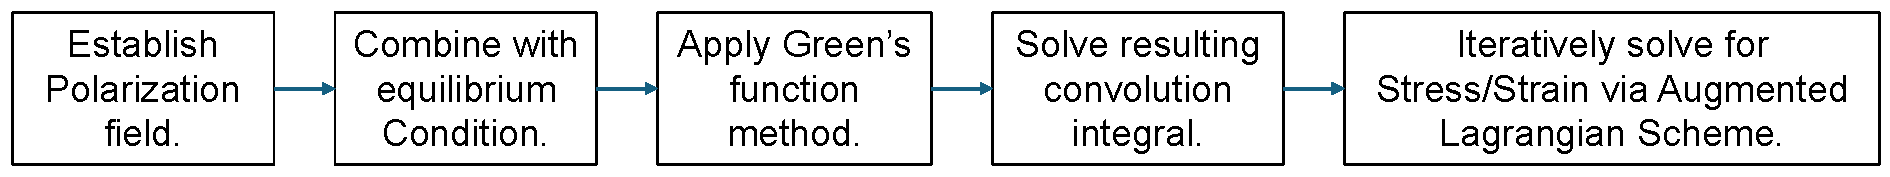
\includegraphics[width=\textwidth]{images/FFT solution procedure.pdf}
    \caption{FFT solution procedure.}
    \label{FFT Solution procedure}
\end{figure}

Fast fourier transform, when compared with FEM, saves on computational effort and time, hence it is used to solve equilibrium equations derived from the crystal plasticity model. The table \ref{Differences between FFT and FEM solvers} shows the differences between FFT and FEM.






\chapter{Literature Review.}
\section{Role of mechanical twinning in plastic deformation of HCP metals.}
Hexagonal Closed Packed lattice itself causes significant anisotropy which has effect on deformation mechanisms. Due to this, hexagonal close-packed metals have the challenge of activating slip along the $\langle c \rangle$-axis at low temperatures and/or high strain rates. Since 4 independent basal slip systems are not enough to accommodate an arbitrary deformation fulfilling von Mises criterion \cite{taylor1938plastic}, twinning will take the role to mediate the plastic deformation in the $\langle c \rangle$-axis taking the role of pyramidal slip systems which are difficult to activate.
Figure \ref{Twin_slip_MG_CRSS} gives the Critical Resolved Shear Stress (CRSS) values. CRSS values quantitatively informs how easy or difficult a particular deformation mode to mediate plastic deformation. The lack of available deformation mechanisms can be qualitatively observed by presence of strong basal texture \cite{Yoo1981409} in cold worked Mg alloys. 
\begin{figure}[H]
    \centering
    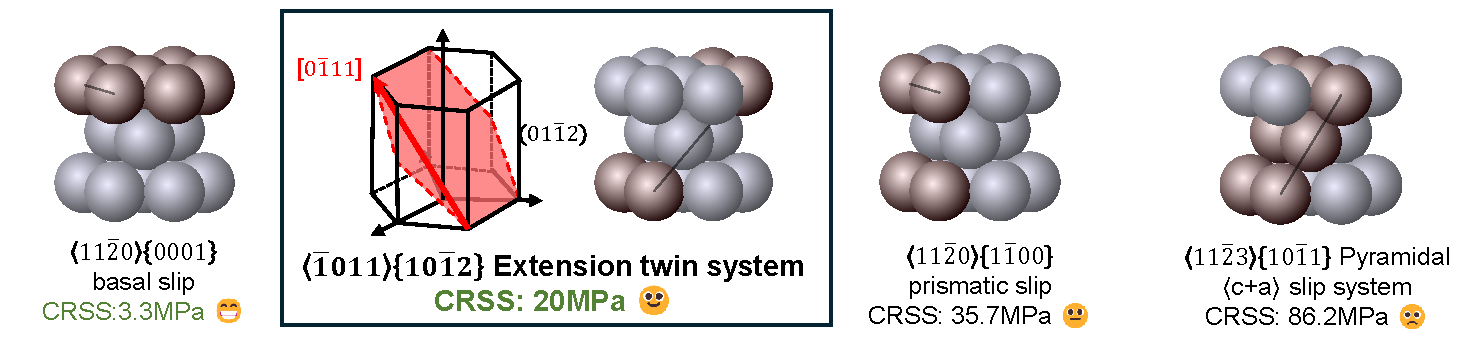
\includegraphics[width=\textwidth]{images/Mg_Deformation_systems_CRSS.pdf}
    \caption{Twin Systems and Slip Systems in Mg and CRSS values}
    \label{Twin_slip_MG_CRSS}
\end{figure}
The relative values of CRSS for slip systems and twin systems play a crucial role in determining whether twinning will contribute significantly to the plastic deformation process or not. The CRSS values for twin systems are lower than those for slip systems, hence twinning is more likely to occur and contribute to plastic deformation. Values of CRSS for different deformation modes at room temperature are given in the Table \ref{CRSS table} \cite{ARULKUMAR2016143} below for Mg\cite{Kelly19685}\cite{BEYERLEIN2011988}, Zr\cite{Knezevic201555}, Ti\cite{QIN2014293}.

\begin{table}[ht]
\centering
\caption{CRSS values of different deformation modes of HCP metals.}
\begin{tabular*}{\textwidth}
{@{\extracolsep{\fill}}c@{\extracolsep{\fill}}*{4}{@{\extracolsep{\fill}}c@{\extracolsep{\fill}}}@{\extracolsep{\fill}}}
\hline
\multicolumn{1}{c}{\textbf{Material}} & \multicolumn{4}{c}{\textbf{CRSS values of slip \& Twin modes}} \\
& Basal $\langle a\rangle$ & Prismatic $\langle a\rangle$ & Pyramidal $\langle c+a\rangle$ & T. Twin \\
\hline
Magnesium     & 3.3  & 35.7  & 86.2 & 20 \\
Zirconium     & 700  & 20    & 160  & 102 \\
Titanium     & 120  & 60    & 180  & 125 \\
\hline
\end{tabular*}

\label{CRSS table}
\end{table}

\section{Experimental observations of deformation twinning.}

\subsection{The stochastic nature of deformation twinning.}
\label{Stochastic_nature}
Beyerlein et al.  \cite{Beyerlein2010StatisticalAO} statistically analysed deformation twinning in magnesium using electron backscatter diffraction (EBSD) data. They found that twinning exhibited inherent statistical variability that could not be explained deterministically.

\begin{figure}[H]
    \centering
    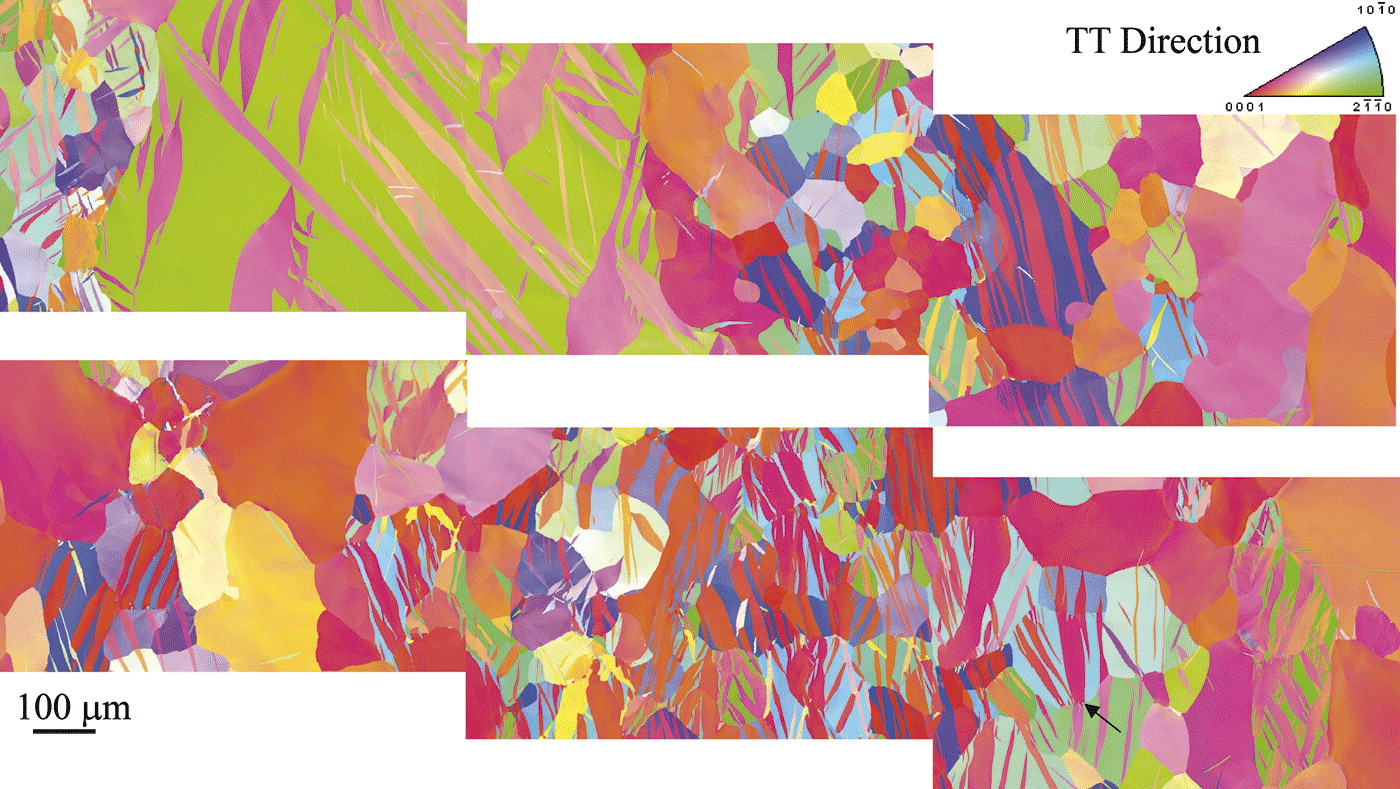
\includegraphics[width=0.7\textwidth]{images/Beyerlein_EBSD.jpg}
    \caption{ Thru-thickness EBSD orientation map of pure Mg @ 3\% compresive strain with $[1 0 \bar{1} 2]$ twinning.}
    \label{fig:8.1}
\end{figure}

Specifically, they observed that twinning occurred in some unexpectedly oriented grains, while more favourably oriented grains did not always twin. The twin variants formed also showed variability and were not always the most geometrically favoured one.

They correlated various microstructural parameters with twinning characteristics. Key findings were:
\begin{itemize}
\item Twinning did not necessarily occur in all similarly sized and oriented grains, conflicting with deterministic rules.
\item The twin variant selected was not always the one with the highest Schmid factor predicted by orientation as shown in figure \ref{fig:8.2}.
\item No clear grain size effect was found on the likelihood of twinning itself, conflicting with Hall-Petch relationships. However, the number of twins per twinned grain increased with grain size as shown in figure \ref{fig:8.2} bottom left.
\item More and thicker twins occurred at small misorientation angle grain boundaries compared to high angle boundaries as shown in figure \ref{fig:8.2} bottom right.
\item Adjoined twin pairs spanning grain boundaries grew thicker than individual twins, likely due to mutual accommodation of strain.
\end{itemize}

\begin{figure}[H]
    \centering
    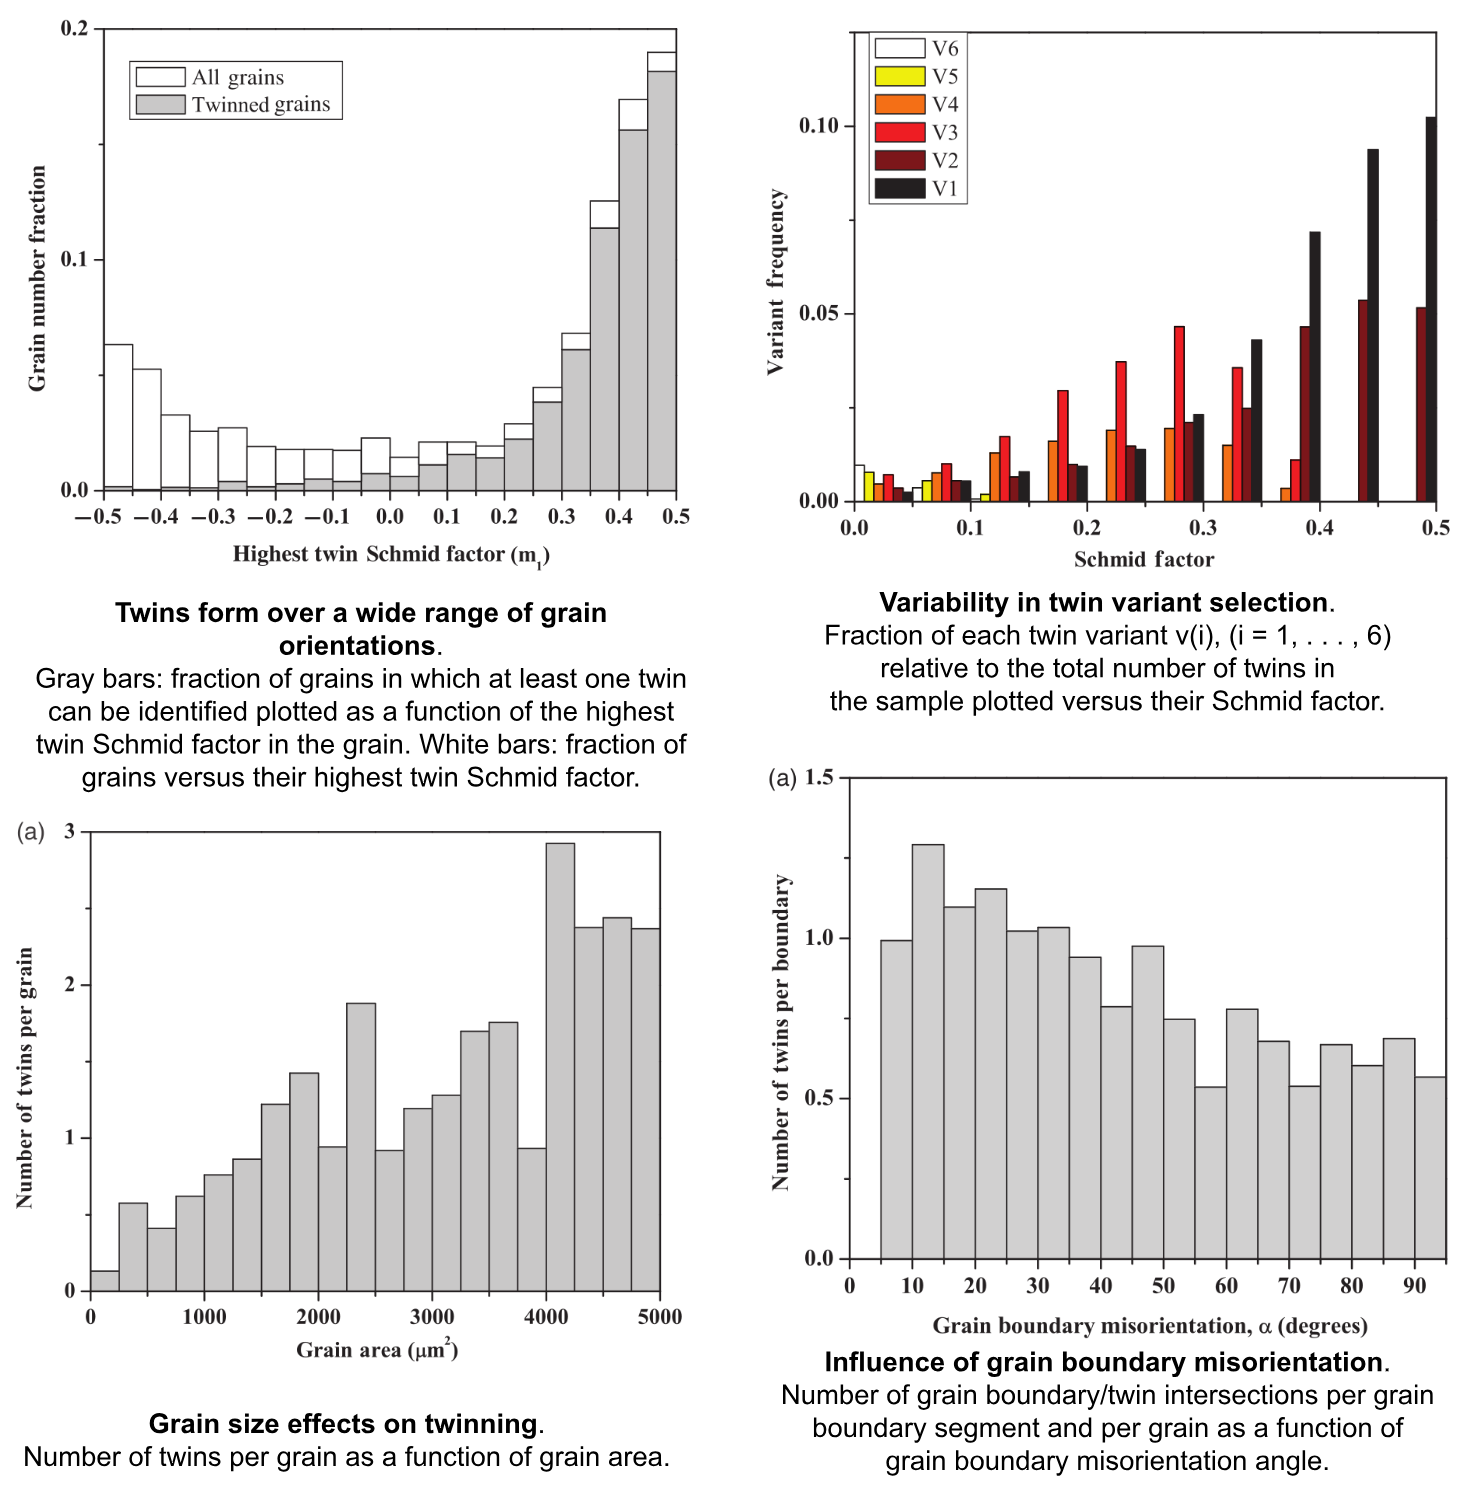
\includegraphics[width=\textwidth]{images/IB02.png}
    \caption{Effects of various crystal structure parameters on formation of twins.}
    \label{fig:8.2}
\end{figure}



\subsection{Twinning crystallography.}
\label{sec:twinning_crystallography}
Geometric description of twinning crystallography given by Christian \cite{CHRISTIAN2002859}, and recent work by Christian and Mahajan \cite{CHRISTIAN19951} is widely used to represent the twinning transformation. Here the twinning transformation is divided into four operations which preserve the symmetry.
\vspace{-0.8em}
\begin{enumerate}
    \item reflection in $K_1$,
    \vspace{-0.8em}
    \item rotation of $180^o$ about $\eta_1$,
    \vspace{-0.8em}
    \item reflection in the plane normal to $\eta_1$, and
    \vspace{-0.8em}
    \item rotation of $180^o$ about the direction normal to $K_1$
\end{enumerate}
\vspace{-0.8em}
Figure \ref{fig:Geomtery of twinning}, Geometry of twinning: We take a section of untwinned crystal sphere parallel to the plane of shear $S$. Sphere is distorted to ellipsoid due to shear $S$ along $\eta_1$ in $K_1$ plane. $\eta^{K1}$ is normal to $K_1$ plane. $K_2$ is the conjugate to the twinning plane and $\eta_2$ direction enclosed in the plane. $K_2^T$ and $\eta_2^T$ represents $K_2$ and $\eta_2$ after transformation due to twinning.

\begin{figure}[ht]
    \centering
    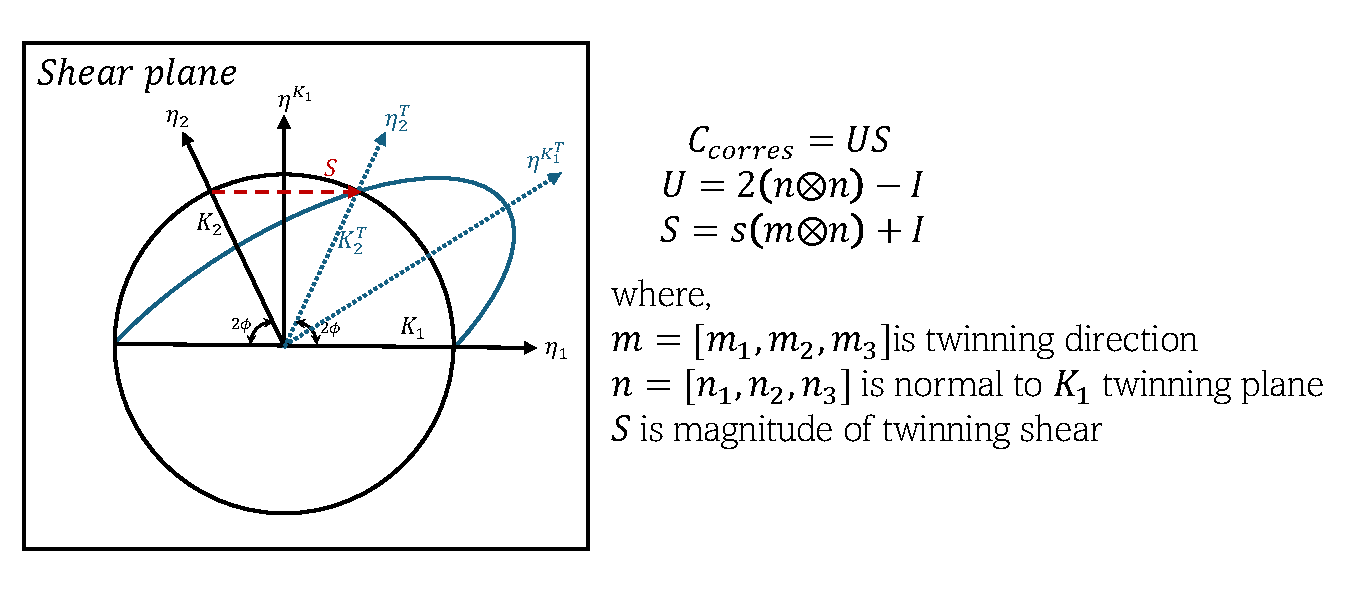
\includegraphics[width=0.95\textwidth]{images/Correspondence_matrix_theory.pdf}
    \caption{Geometrical representation of twinning.}
    \label{fig:Geomtery of twinning}
\end{figure}

\subsubsection{Quantifying the crystallographic transformation of deformation twinning in the framework of Crystal Plasticity.}

Niewczas\cite{Niewczas121} has developed deformation, re-indexation, \& correspondence matrices that quantify the lattice transformation associated with different twinning modes in hexagonal close-packed (hcp) metals. Specifically, the matrices describe the shear and rotation of lattice vectors and planes that occur when mechanical twinning operates.

These matrices can directly inform the kinematic formulations in a crystal plasticity model to capture twinning:
\begin{itemize}
\item The deformation matrix $S$ encapsulates the homogeneous shear strain produced by twinning along a specific twin mode. This defines the deformation gradient for twinning. \\ $S = s(m\otimes n)-I$ where $s$ is magnitude of twinning shear, \\ $m = [m_1,m_2,m_3] \ is \ twinning\ direction.$, and \\ $n = [n_1,n_2,n_3] \ is \ normal\ to\ K_1\ plane.$
\item The re-indexation matrix $U$ captures the crystal reorientation due to twinning. It provides the rotation component for updating the orientation of a twin domain. \\ $U = 2(n\otimes n)-I$
\item The correspondence matrix C consolidates the effects of both deformation and reorientation through twinning. C maps lattice elements from the parent to twin lattice and vice versa. \\ $C_{corres} = US$
\end{itemize}

By incorporating these transformation rules into the kinematic description, a crystal plasticity model can explicitly represent the lattice distortions that accompany the formation of a twin domain. This level of crystallographic detail enables more accurate modelling of mechanical twinning in hcp metals.

\section{Crystal plasticity models on deformation twinning.}

Over the past decades, numerous crystal plasticity models, which incorporate twinning, have been developed. However, the majority of these models have adopted a phenomenological, volume fraction-based approach to pseudo-twinning, which is spatially homogenised. While this approach may be suitable for predicting average texture and certain macroscopic properties, it has limited capability in capturing the micromechanical consequences of highly localised deformation caused by twinning, such as damage, early localization, and most importantly, the interaction between dislocation slip and twinning.

Recently, phase field modelling has demonstrated significant potential in modelling spatially resolved mechanical twinning, providing a clear interface between parent and twin orientations. However, this approach prohibitively expensive in terms of computational time and power.

Given these facts, a gap exists in the field of efficient modelling of deformation twinning using continuum approaches. Addressing this gap is essential to enhance our understanding of deformation twinning in HCP metals.

\subsection{Available crystal plasticity models for deformation twinning.}

Although twinning and slip are both responsible for plastic deformation in HCP metals. Twinning once nucleated will act at different lenghscale and timescale. Hence incorporating twinning along with slip in CP models has been always been a challenge. A chronological account of major attempts to model is presented here based on existing review article by Paudel et al \cite{Paduel202111091373}.
\vspace{-0.8em}
%Existing Crystal Plasticity Models which incorporates deformation twinning can be classified to 2 categories:
%1. Volume Fraction based approaches.
%2. Energy based and phase field approaches.
\subsubsection{1969-1978: Early attempts}
\vspace{-0.8em}
Earliest pioneering work for modelling deformation twinning was done by Chin et al. in 1969 \cite{Chin1969.0051} for cubic materials based on Taylor’s least work hypothesis\cite{taylor1938plastic}. Based on this work earliest successful simulation of deformation twinning for Brass was done by Van Houtte in 1978\cite{HOUTTE1978591} texture evolution based on the load-deformation relationship was successfully modelled for the first time. Also the concept of twinned ``\textbf{volume fraction}" was introduced for the first time. Volume fraction of twin, which is derived from the local shear stress, physically represents the fraction of twinned volume in the total volume of a specific democratized element. It is a continuous quantity which varies from 0 to 1. Volume fraction allows a discrete entity which causes discontinuity to be modelled in the continuum mechanics framework. %Additionally, in this model, they reorient the twinned grain based on Monte Carlo scheme and choose the variant of twin based on a probabilistic criteria.
\vspace{-0.8em}
\subsubsection{1991: Predominant Twin Reorientation and Volume Fraction Transfer}
\vspace{-0.8em}
Modeling deformation twinning in HCP metals was first done by Lebensohn et al. in 1991 \cite{Lebensohn1991ModellingTI}, where they improved the previous model by their ``Predominant Twinning Reorientation"(PTR) scheme which was improved again in 1991 by Tome et al.\cite{TOME19912667} when they model Zirconium. They call this as ``Volume Fraction Transfer" (VFT) scheme. These schemes use deterministic criteria where they select most dominant variant for completely(PTR) or partially(VFT) reorientation of the grain. The PTR-VFT scheme predicts texture evolution better than the the previous model.
\vspace{-0.8em}
\subsubsection{1998: Twinning as ``Pseudo Slip" in Lagrangian Framework.}
\vspace{-0.8em}
Kalidindi's Lagrangian incorporation of twinning\cite{KALIDINDI1998267} in 1998 was one of the important approaches to model the deformation twinning which is still used today in DAMASK. In this approach twinning is considered as pseudo-slip and it incorporates deformation caused by the twinning into the kinematics of the Lagrangian framework. This model is very efficient because it mainly aims to predict the stress-strain response bypassing the prediction of texture evolution.
\vspace{-0.8em}
\subsubsection{2007: Composite Grain approach}
\vspace{-0.8em}
Proust in 2007 \cite{PROUST20072137} makes an improvement for PTR-VFT scheme. In this model a crystal or grain is treated as a composite material made with matrix and twin lamellae which evolve with deformation. Here the hardening laws incorporate the twin-slip interaction making use of geometrically necessary dislocations and a directional Hall–Petch mechanism. It provides a better prediction of internal stresses and strains within a grain.
\vspace{-0.8em}
\subsubsection{2008: Dislocation-density based model}
\vspace{-0.8em}
Beyerlein and Tomé in 2008 \cite{BEYERLEIN2008867} developed a dislocation-density based model to link twinning with the evolution of dislocation density which gives a more comprehensive understanding on the effect of temperature transition from slip dominated to twinning dominated deformation.
\vspace{-0.8em}
\subsubsection{2010: Probabilistic twin nucleation model}
\vspace{-0.8em}
Beyerlein and Tomé in 2010\cite{beyerlein2010probabilistic} developed probabilistic nucleation framework to which addresses the stochastic nature of twinning. This gives much more realistic description of nucleation events leading to more accurate prediction of deformation behavior.
\vspace{-0.8em}
\subsubsection{2012: Twinning-Detwinning}
\vspace{-0.8em}
Wang et al \cite{WANG201293} proposed this model to address the detwinning behavior observed during reversed loading, which was not captured by previous models.
\vspace{-0.8em}
\subsubsection{2015-2017: Energy based approach for twin nucleation and evolution.}
\vspace{-0.8em}
This model is described in series of publications by Cheng et al.\cite{CHENG2015148}\cite{CHENG2017512}. Here energy of interactions between crystal defects are considered and energy for dislocation dissociation is considered as nucleation criteria. Twin propagation is based on thermal energy calculated from shearing and shuffling of atoms. 
\vspace{-0.8em}
\subsubsection{2014-2021: Phase Field Twinning Model}
\vspace{-0.8em}
In this very recent approach by Kondo et al. 2014 \cite{KONDO2014672} and Liu et al.  Twin and parent regions are treated as different phases described by an order parameter $\eta$. Stochastic methods are used for twin nucleation mechanism and the evolution of the twin order parameter driven by discrete twin interface energy. This enables modeling of complex twin morphologies and their interactions with other microstructural defects.

\vspace{0.5em}
These models can be broadly classified to two groups:
\vspace{-0.8em}
\begin{enumerate}
    \item Volume fraction based approaches.
    \vspace{-0.8em}
    \item Energy based or phase field approaches.
\end{enumerate}
%\vspace{-0.8em}
Volume fraction based approaches have been less accurate to predict either texture evolution or load-deformation response, and Energy based or phase field approaches have been less computationally efficient.

The table \ref{Comparision of CP models for twinning} gives the summary of all the literature regarding different Crystal Plasticity models which were reviewed for this work.


\begin{table}[H]
  \centering
  \caption{Comparision of different CP models for twinning.}
  \renewcommand\arraystretch{1.2}
  \renewcommand\baselinestretch{1.2}
  \begin{tabular}{|m{4.2cm}|m{7.8cm}|c|}
    \hline
    CP Model & Model Features & Remarks \\
    \hline
    Predominant twin reorientation \cite{HOUTTE1978591} & Predicts texture evolution using predominant twin system & \multicolumn{1}{|c|}{\multirow{15}{2cm}{Volume Fraction based, less accurate}} \\
    \cline{1-2}
    Volume Fraction Transfer \cite{TOME19912667} & PTR + volume fraction variable for accurate prediction of texture. & \multicolumn{1}{|c|}{} \\
    \cline{1-2}
    Kalidindi's Lagrangian method.\cite{KALIDINDI1998267} & Incorporates twinning as ``pseudo-slip" in kinematics based on evolution of volume fraction. & \multicolumn{1}{|c|}{} \\
    \cline{1-2}
    Updated Lagrangian method \cite{LEVESQUE201065} \cite{Lebensohn.2003.1212} & Also incorporates secondary twins and slips and tertiary slip. & \multicolumn{1}{|c|}{} \\
    \cline{1-2}
    Composite Grain model \cite{PROUST20072137} \cite{PROUST2009861} & Incorporates effect of SSD, GND and Hall-Petch effect at twin interfaces. & \multicolumn{1}{|c|}{} \\
    \cline{1-2}
    Twinning detwinning model \cite{WANG201293} \cite{WANG201336} & Incorporates detwinning in a CP model to simulate hysteresis & \multicolumn{1}{|c|}{} \\
    \cline{1-2}
    Dislocation-density based model \cite{BEYERLEIN2008867} \cite{Knezevic201555} & Includes dislocation transmutation and twin accommodation effects to predict plastic anisotropy. & \multicolumn{1}{|c|}{} \\
    \cline{1-2}
    Probabilistic nucleation method \cite{beyerlein2010probabilistic} \cite{BARNETT2015151} & Based on numerical observation from atomistic simulations and statistical analyses. & \multicolumn{1}{|c|}{} \\
    \cline{1-2}
    Explicit incorporation method \cite{ABDOLVAND2013783} \cite{ARDELJAN2015396} & Twin is explicitly incorporated by remeshing RVE before every timestep to achieve spatially resolved fields & \multicolumn{1}{|c|}{} \\
    \hline
    Energy based micro-twin nucleation model \cite{CHENG2015148} \cite{PARAMATMUNI2020102778} & Based on energy of dislocation interaction. Predicts heterogeneous twin formation with strain localization. & \multicolumn{1}{|c|}{\multirow{3}{2cm}{Energy based approaches, Computationally expensive}} \\
    \cline{1-2}
    Thermal activation based twin propagation method \cite{CHENG2017512} \cite{Ghosh2018} & Nucleation based on thermal energy activation which accounts for shear-shuffle process. & \multicolumn{1}{|c|}{} \\
    \cline{1-2}
    Phase field twinning model \cite{KONDO2014672} \cite{GRILLI2020104061} & Twin evolution as a phase transformation of parent into twin. Based on Gibbs energy. & \multicolumn{1}{|c|}{} \\
    \hline
  \end{tabular}
  \label{Comparision of CP models for twinning}
\end{table}

\section{Software for Crystal Plasticity modeling and simulation.}
There are many software available to create constitutive models and run simulations. Based on license we can classify them as commercial and open source.

List of some commercial software:
\vspace{-0.8em}
\begin{itemize}
    \setlength\itemsep{-0.5em}
    \item ABAQUS
    \item ANSYS
    \item MSC(MARC)
    \item COMSOL
\end{itemize}
\vspace{-0.8em}
List of some opensource software:
\vspace{-0.8em}
\begin{itemize}
    \setlength\itemsep{-0.5em}
    \item DAMASK
    \item PRISMS
    \item MOOSE
    \item FEniCS
    \item FreeFEM
\end{itemize}

For the choice of implementation of our model we compare various software available to us as given in the table \ref{CP-Software-Comparision}.

\begin{table}[H]
\centering
 \caption{Comparison of some notable software used for Crystal Plasticity Simulations.}
\begin{tabular}{ |m{4.3em}||m{4.2cm}|m{2.5cm}|m{1.7cm}|m{2.7cm}| }
 \hline
 & \multicolumn{4}{|c|}{Features} \\
 \hline
 Software& Developer(s) & License & Language & Solver Choices \\
 \hline \hline
 DAMASK &Max-Planck-Institut für Eisenforschung GmbH&Open Source&Fortran& FFT and FEM \\ %(Implicit)
 \hline
 ABAQUS&Dassault Systèmes&Proprietary /commercial&Fortran&FEM \\ %(Implicit and Explicit)
 \hline
 MOOSE &Idaho National Lab&Partially Open Source&C++&FEM \\ %(Implicit and Explicit)
 \hline
 PRISMS / deal.II&University of Michigan / Universität Heidelberg&Open Source&C++& FEM \\ %(Implicit and Explicit)
 \hline
 FEniCS &(Multiple) &Open Source&C++ \& Python& FEM \\ %(Implicit and Explicit)
 %\hline
 %WARP3D&University of Illinoi&Open Source & FEM\\
 \hline
\end{tabular}

 \label{CP-Software-Comparision}
 \end{table}
 
\subsubsection{The choice of DAMASK.}
From the review of different software packages available, we make an informed choice for implementing our discrete twin model. DAMASK is chosen as it gives choice of 2 solvers to test our model. DAMASK is modular and implementation of our model does not affect the other components of the code. At the same time DAMASK integrates all the modules such that it gives access to most internal subroutines and functions, the state container to store and manipulate results, and neighbouring elements or integration points. We utilize these features in our model.

\section{DAMASK.}
DAMASK (Düsseldorf Advanced Material Simulation Kit) \cite{ROTERS2019420}, an open source software developed by the Max-Planck-Institut für Eisenforschung, to implement our discrete twin model due to its powerful capabilities in multi-physics crystal plasticity simulations. One of the key advantages of DAMASK is that it is open source, allowing us to directly access and modify the source code to build customized features and models into the software.

\subsection{Concept:}
DAMASK provides tools to solve the constitutive response that connects deformation and stress at each material point based on Crystal Plasticity using a variety of constitutive models and homogenization approaches. DAMASK is capable of handling multi-physics problems, following a modular approach, additional field equations containing displacive phase transformation, significant heating, and potential damage evolution are solved in a fully coupled way. 

DAMASK was developed to emulate the multi-scale hierarchy and multi-physics structure observed in the material physics of thermo-mechanical loading of complex materials. Consequently, it defines template functions that link numerical solvers, homogenization methods, and constitutive laws. To increase flexibility, one can combine various constitutive laws and homogenization schemes, along with a specific set of solvers for the associated boundary and/or initial value issues, in the same model.
\subsubsection{Hierarchical structure of different modules:}
Damask is a modular software with a hierarchical structure
\begin{figure}[H]
    \centering
    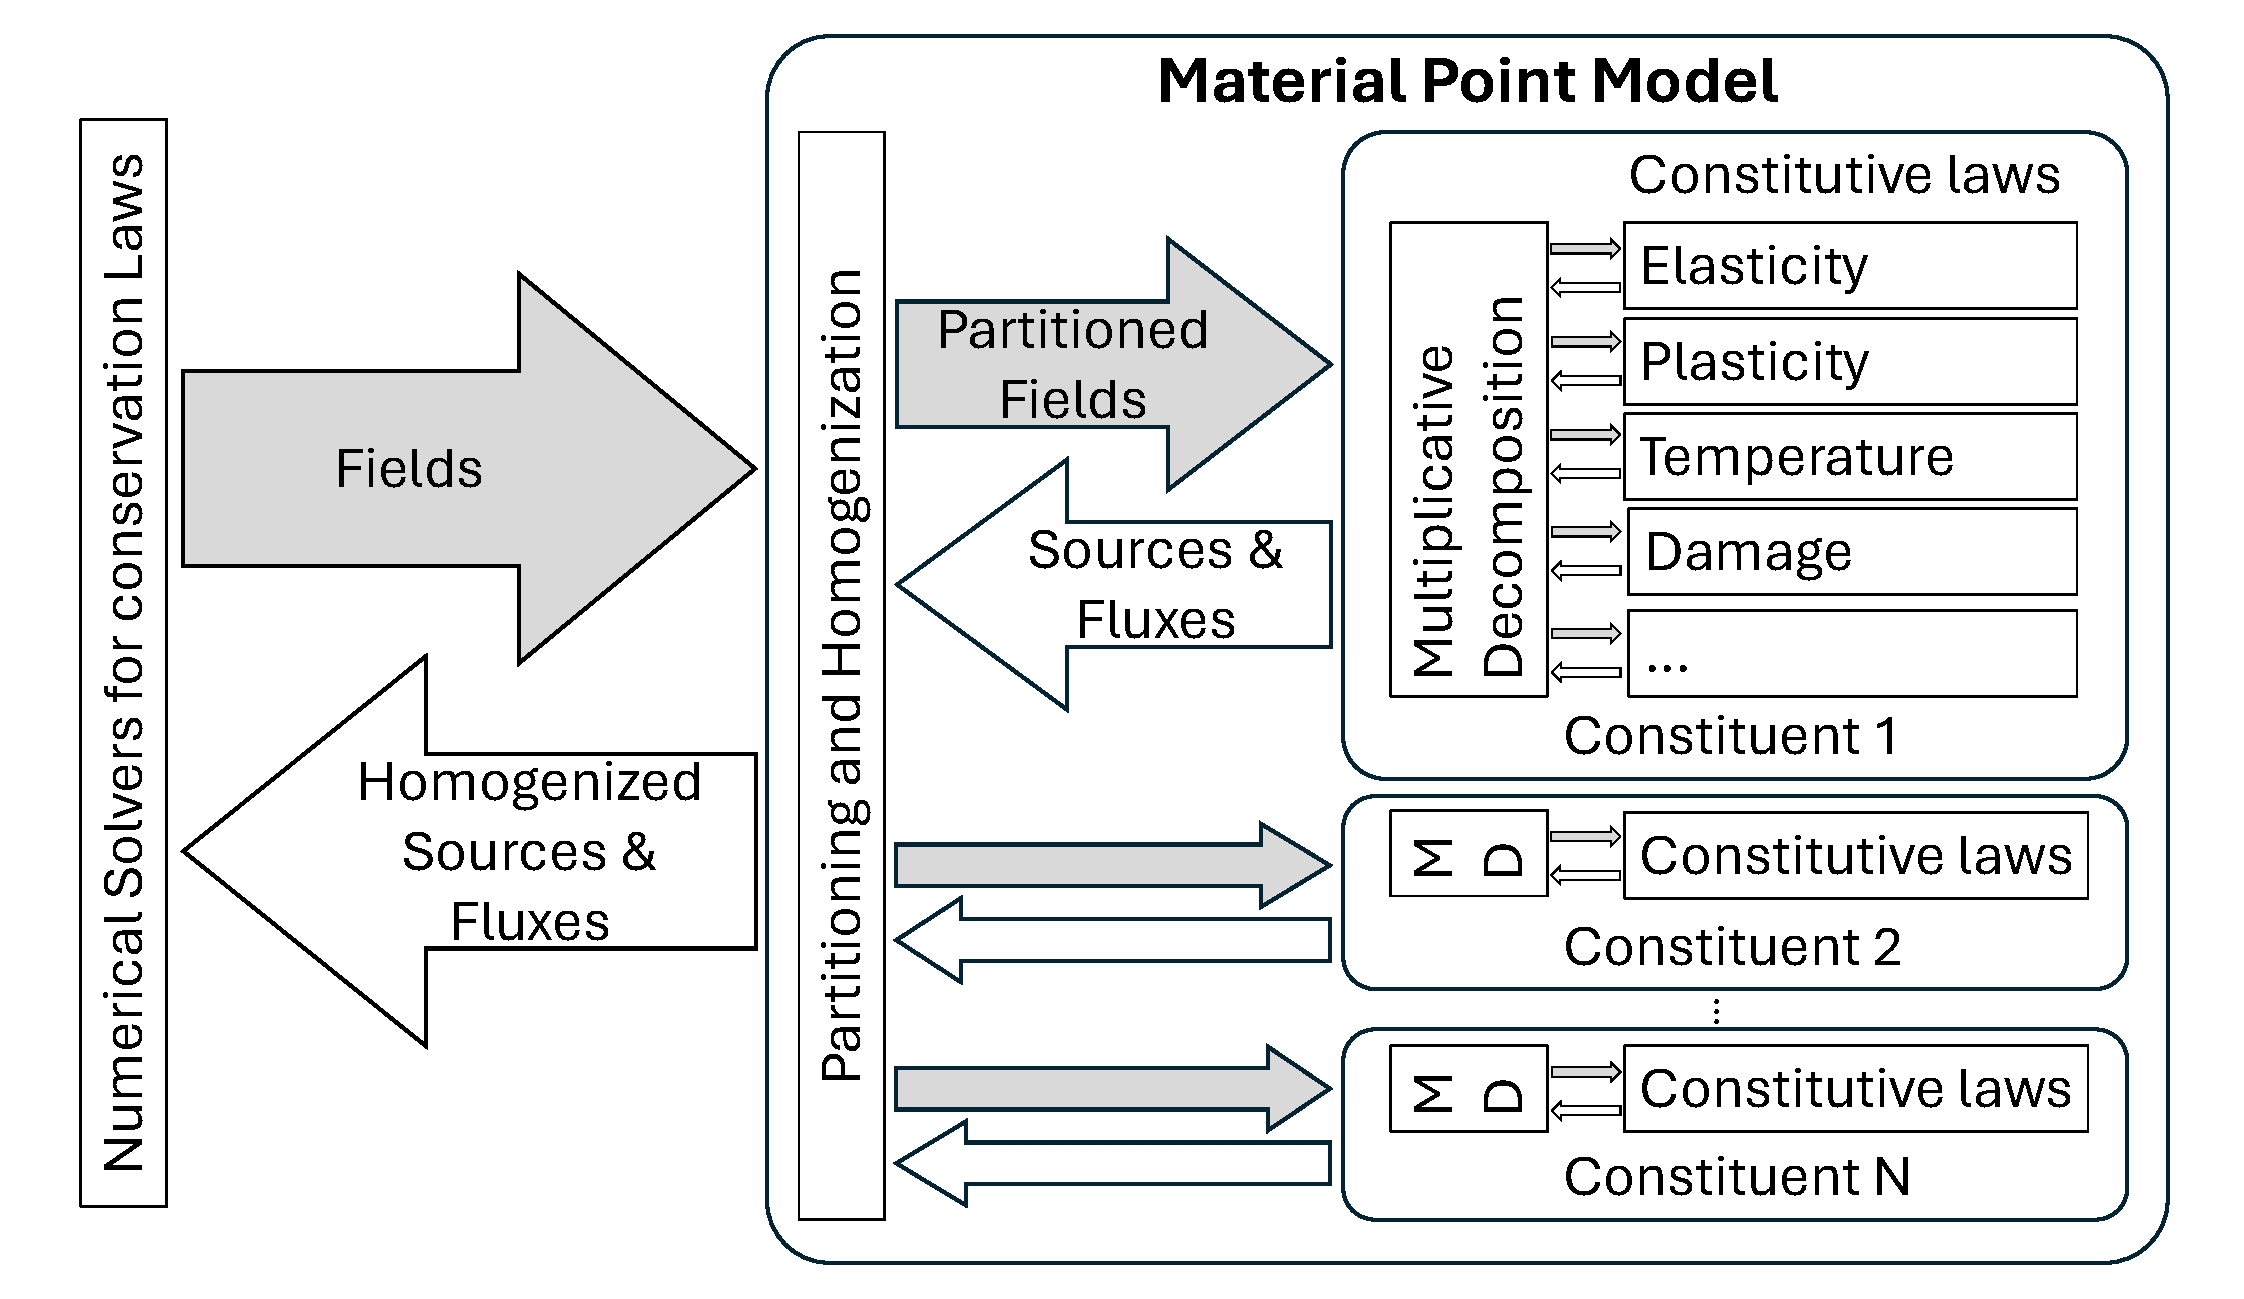
\includegraphics[width=\textwidth]{images/Hierarchical structure of DAMASK at a material point.pdf}
    \caption{Hierarchical structure of DAMASK at a material point}
    \label{DAMASK_hierarchy}
\end{figure}


The conservation laws in DAMASK require a structured multi-scale description of the fluxes and sources across hierarchical levels. At the highest level, a division and homogenization scheme partitions prescribed field values on a material point among its underlying microstructural elements and subsequently homogenizes each constituent's constitutive reaction. At the intermediate Constituent Level, time integration of the underlying constitutive laws determines the reaction of each microstructural constituent in terms of fluxes and sources. Finally, at the lowest level, constitutive laws based on evolving internal state variables provide this response.
\subsection{Constitutive Models:}
Constitutive models form the foundational blocks of DAMASK's hierarchical structure, characterized by internal state variables that capture history dependence.
\subsubsection{Elasticity}
The elastic behavior is modeled using a Generalized Hooke's Law that relates the Second Piola-Kirchhoff stress $S$ and Green-Lagrange strain $E$ through an elastic stiffness matrix $\mathbb{C}$. 
\begin{equation}
    S = \mathbb{C} : E\
\end{equation}
\subsection{Plasticity:}
The crystal plasticity laws provide the plastic velocity gradient $L_p$ for a given Mandel stress $M_p$.
\subsubsection{Phenomenological Crystal Plasticity in DAMASK:}
In polycrystalline materials, plastic deformation occurs on well-defined planes and directions dictated by the lattice structure. The total plasticity is calculated as the sum of the shear rates from the individual slip systems according to the following equation:
\begin{equation}
    L_p = \sum_{\alpha} \dot{\gamma} ^\alpha \underbrace{(s_{S}^{\alpha} \otimes n_{S}^{\alpha})}_{=:P_{Schmid}^{\alpha}}
\end{equation}
s and n are the directions and Normal's to the slip planes. Schmid's law provides the expression for the resolved shear stress which acts as driving force for plastic slip:
\begin{equation}
 \tau^\alpha=M_p . P_{Schmid}^{\alpha}
\end{equation}
The modified form of Phenomenological Crystal Plasticity introduced by Hutchinson for FCC and extended to twinning by Kalidindi is used in DAMASK. The plastic component in the internal variables represents resistances to slip and twinning. It is characterized by the equation:
\begin{multline}
\dot{\xi}^{\alpha}=h_{0}^{s-s}(1+c_1(f_{tw}^{tot})^{c_2})(1+h_{int}^{\alpha}) \\ *
\sum_{\alpha'=1}^{N_s} \lvert\dot{\gamma}^{\alpha'}\rvert \bigg|1-\frac{\dot{\xi}^{\alpha'}}{\dot{\xi}^{\alpha'}_{\infty}}\bigg|^{\alpha} sign\bigg(1-\frac{\dot{\xi}^{\alpha'}}{\dot{\xi}^{\alpha'}_{\infty}}\bigg)h^{\alpha\alpha'}+\sum_{\beta'=1}^{N_tw} \dot{\gamma}^{\beta'}h^{\alpha\beta'}
\end{multline}
Where $f_tot_tw$ represents the twin volume fraction and h covers the slip-slip and slip-twin interaction parameters. The remaining terms are model fitting parameters. Likewise, the evolution of resistances on twin systems is given by:
\begin{equation}
\dot{\xi}^{\beta}=h_{0}^{tw-s}(\sum_{\alpha=1}^{N_s}\lvert\dot{\gamma}^{\alpha}\rvert)^{c_3} \sum_{\alpha'=1}^{N_s}\lvert\dot{\gamma}^{\alpha'}\rvert h^{\beta\alpha'} + h_{0}^{tw-tw} (f_{tw}^{tot})^{c_4}  \sum_{\beta'=1}^{N_tw} \dot{\gamma}^{\beta'}h^{\beta\beta'}
\end{equation}

The evolution of shear rate on each slip system is given by,

\begin{equation}
\dot{\gamma}^{\alpha} = (1-f_{tw}^{tot}) \dot{\gamma}^{\alpha}_{0} \bigg| \frac{\tau^\alpha} {\xi^\alpha} \bigg|^n sgn(\tau^\alpha)
\end{equation}

The evolution of shear rate due to mechanical twinning takes into account the unidirectional character of twin formation:

\begin{equation}
\dot{\gamma} = (1-f_{tw}^{tot}) \dot{\gamma}_{0} \bigg| \frac{\tau}{\xi} \bigg|^n \mathcal{H}(\tau^\alpha)
\end{equation}

where $\mathcal{H}$ is the heaviside or unit step function. The total twin volume fraction is given by,

\begin{equation}
f_{tw}^{tot} = max \left(  \sum_{\beta=1}^{N_{tw}} \underbrace{\frac{\gamma^{\beta}}{\gamma^{\beta}_{char}}}_{=:f^{\beta}_{tw}},1.0 \right)
\end{equation}
where $\gamma_{char}$ is the characteristic shear dye to mechanical twinning, the value of which depends on the twin system.

%dgmdt(is) = shrt_0*abs(tau_eff(is)/IVB_eff(is)))**pw_fl*sign(1.d0,tau_eff(is))

%This behavior is described by the constitutive equation \eqref{eq:shear_strain_rate}

%\eqref{eq:shear_strain_rate}

%\begin{equation}
%\dot{\gamma} = \dot{\gamma}_{0} \left| \frac{\tau_{eff}}{\tau_{Ceff}} \right|^n \operatorname{sign}(\tau_{eff})
%\end{equation}

% ddgmdt_dtau(is) = pw_fl/IVB_eff(is)*shrt_0*(abs(tau_eff(is)/IVB_eff(is)))**(pw_fl-1)

%\begin{equation}
%    \frac{\dot{\gamma}}{\dot{\tau}} = \frac{n}{\tau_{eff}} \dot{\gamma}_{0} 
%\end{equation}

%\begin{equation}
%\dot{\gamma} = \dot{\gamma}_{0} \left| \frac{\tau_{eff}}{\tau_{Ceff}} \right|^n \operatorname{sign}(\tau_{eff}) \label{eq:shear_strain_rate}
%\end{equation}

% ddgmdt_dIVB(is) = -pw_fl*dgmdt(is)/IVB_eff(is)

% ddIVBdt_dIVB(is,js) = crsF_mat(is,js)*hdrt_0*ddgmdt_dIVB(js)*sign(1.d0,tau_eff(js))*x1**pw_hd - crsF_mat(is,js)*hdrt_0*abs(dgmdt(js)) *x1**(pw_hd-1)*pw_hd/crss_s


\chapter{Development of the Discrete Twinning constitutive model.}
The discrete twinning model incorporates a spatially resolved representation of twinning events, aligning with experimental observations. Unlike volume fraction-based approaches where material points can simultaneously exhibit both twinned and untwinned states, the discrete model restricts each point to either the twinned or untwinned (parent) state similar to an order parameter in phase field modelling.

This discrete twinning model can couple with existing crystal plasticity formulations in the multiphysics DAMASK simulation package \cite{ROTERS2019420}. While the crystal plasticity component handles deformation from dislocation slip, the discrete twinning portion specifically captures the mechanical twinning contribution. By segregating the slip and twinning behaviours, the model provides more physical fidelity and flexibility compared to conventional phenomenological implementations. Overall, the discrete twinning approach enables targeted insights into the distinct twinning phenomenology while seamlessly integrating with DAMASK's extensive crystal plasticity multi-physics modelling capabilities.

\section{Assumptions made in the discrete twinning model.}

\begin{itemize}
\item Grain boundaries are assumed to be the location of nucleation events.
\item We consider all the discretized material points (FFT voxel or FEM element) which are neighbouring to twinned elements for growth of the twin.
\item All the discretized material points which are considered for nucleation or growth are assigned a random number. The random number assigned is uniformly distributed between 0 and 1.
\item Since twinning frequency and variant selection frequency are strongly correlated with Schmid factor, we consider volume fraction which is derived using Schmid factor as the criteria for declaring the discretized material point as discretely twinned. 
\item The twin events are considered as instantaneous and the discretized material point is flipped at the same time step.


\end{itemize}

\section{Incorporating the stochastic nature of the deformation twins.}

As we have seen in the literature review section \ref{Stochastic_nature}, deformation twinning is inherently stochastic process, and to model this we use random sampling technique inspired by the Monte Carlo Method.

\subsection{The Monte Carlo method}

Monte Carlo methods are widely used computational techniques that estimate solutions to problems that are challenging or impractical to solve using deterministic methods. They achieve this by employing repeated random sampling, drawing randomly generated numbers as inputs to simulate a wide range of potential outcomes.

In Monte Carlo methods, randomness is used to provide estimates of deterministic quantities. A simple application of this numerical technique is the estimation of the area between two curves.

Consider the following two curves: \\
Curve 1: $y = 2x$ \\
Curve 2: $y = x^2$

To estimate the area between these two curves using the Monte Carlo method, we first define the limits of the region (the bounding rectangle) that encloses the area of interest. In this case, the limits are set to $x_{min} = 0,\ x_{max} = 2,\ y_{min} = min(func1(x_{min}),\ func2(x_{min})),$ and $y_{max} = max(func1(x_{max}),\ func2(x_{max}))$.

The Monte Carlo simulation is performed by generating a large number of random points within the bounding rectangle domain. For each random point, we check if it falls within the area between the two curves by evaluating the conditions: $ y_{min} \leq y \leq max(func1(x),\ func2(x)) $ and $ min(func1(x),\ func2(x)) \leq y $.

\begin{figure}[H]
  \centering
  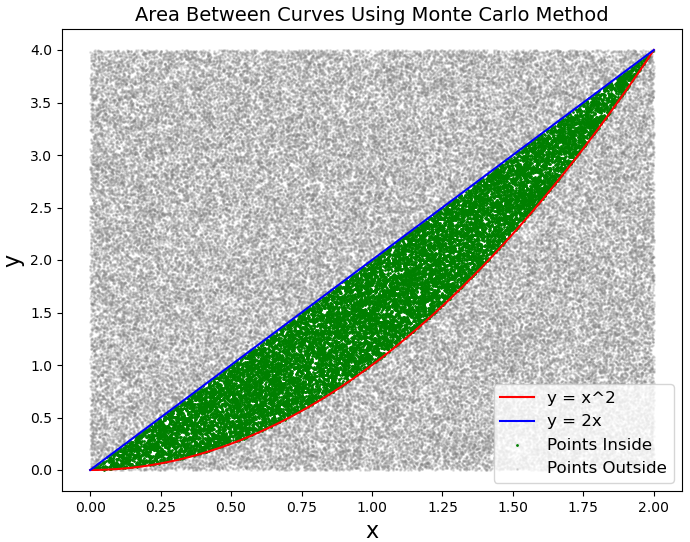
\includegraphics[width=0.6\textwidth]{images/monte_carlo_area.png}
  \caption{Simple application of monte carlo method}
  \label{Monte_carlo_app}
\end{figure}


The ratio of points inside the area to the total number of points, multiplied by the area of the bounding rectangle, gives an estimate of the area between the curves.
\[
\textbf{Area\ between\ the\ curves} = \frac{Points\ inside\ the\ area}{Total\ number\ of\ points} * {Area\ of\ the\ bounding\ rectangle}
\]
The accuracy of the estimated area depends on the number of random points generated. Increasing the number of points will generally lead to a more accurate estimate, but it will also increase the computation time.

\subsection{Random sampling technique applied in the discrete twin model.}
The twinning is inherently stochastic in nature; we introduce stochasticity to our model using a random sampling method (similar to Monte Carlo method) to determine if a particular material point is activated for twin nucleation or growth. At each time step all the material points in the parent crystal are assigned a random number between 0 and 1. For each material point where the random number is compared using a predefined criteria. Based on the outcome of this, the material point is given a discrete state of twinning: either twinned or not twinned. The criteria we use is the local stress-driven evolution of the twin volume fraction for a specific twin system, obtained per the equation from Kalidindi's model \cite{KALIDINDI1998267}:

\[
\dot{f}_\text{twin}^\beta = 
\begin{cases}
\dot{\gamma}_0 \left(\lvert \tau^\beta \rvert/\tau^{\beta}_c\right)^n/\gamma^c_\text{twin} & \text{if } \tau^\beta > 0 \\\\
0 & \text{if } \tau^\beta \leq 0
\end{cases}
\]

where $\tau^{\beta}$ , $\tau_c^{\beta}$ , $\gamma_{twin}^c$ represent stress driving force, critical resolved shear stress (CRSS) for twinning and characteristic shear due to mechanical twinning.

If the sampling outcome is “failure," no changes occur and sampling continues. If the outcome is “success," the material point state flips immediately to the twinned state, the consequences of which are discussed in section .

\subsection{Sampling parameters.}
\subsubsection{Frequency of sampling.}

 \begin{figure}[H]
    \centering
    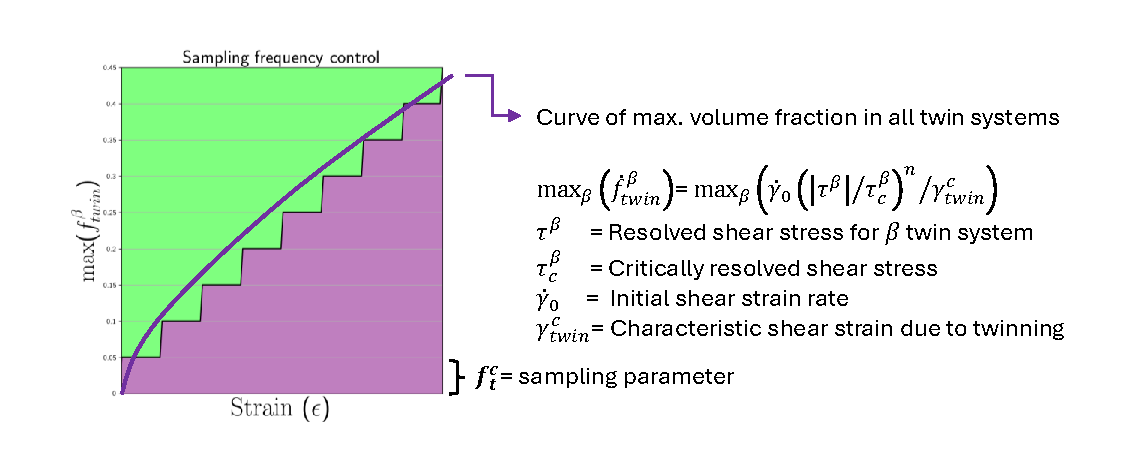
\includegraphics[width=\textwidth]{images/Sampling_parameter.pdf}
    \caption{Scheme to control sampling frequency.}
    \label{Sampling_frequency}
\end{figure}

 If a voxel is sampled more times it has more chances of getting twinned. In other words, Frequency of sampling of the voxel determines probability of twinning. In the discrete twin model, if a voxel is sampled once, we make it harder for it to sample it again by increasing a parameter. This follows the evolution of the maximum volume fraction of all the twin systems. The schematic representation of this is given in figure \ref{Sampling_frequency}.
 
\subsubsection{Distribution of random number.}
 The distribution or range of the random number can be regulated relative to the volume fraction to control the onset of sampling. For instance, if the range of random numbers is restricted between 0.4 and 1, then sampling will only commence after the volume fraction reaches 0.4 for the voxel. This is analogous to expanding or contracting the domain over which random sampling occurs. It resembles adjusting the size of the bullseye in a dart game.

\subsection{Separate treatment of nucleation and growth of twins.}

\begin{wrapfigure}{rH}{0.45\textwidth}
    \centering 
    \resizebox{0.4\textwidth}{!}{
    \includesvg[width=0.4\textwidth]{images/Twin_events_schematic.svg}}
    \caption{Twinning events schematic.}
    \caption*{\ \ First a grain boundary element is twinned and neighbouring elements are selected for growth. For thickening of twin, subsequent neighbours are selected.}
    \label{fig:Twinning_events}
\end{wrapfigure}

We treat nucleation and growth events separately.

The nucleation events are assumed to happen at grain boundaries following the work of Beyerlein(2010) \cite{beyerlein2010probabilistic}. Nucleation occurs independently at grain boundaries, with volume fraction driven by local stress as the sole criteria for event initiation.

The growth events which includes propagation and band thickening is done by method similar to Cheng(2017) \cite{CHENG2017512}, where neighbouring elements are identified and the maximum volume fraction of all twin systems is compared with the random number assigned for that voxel. Growth only proceeds if at least one neighboring point is already twinned, making neighbor state (twinned or untwinned) which is decided by random sampling parameters.

\subsubsection{Selection of Neighbouring Voxels/Elements.}
We select neighbouring voxels using a ``do" loop which loops from ONE to total number of neighbours. In a structured hexahedral grid, the number of neighbours adjacent to 6 faces of element are 6, the loop runs from 1 to 6. ``IPneighborhood" function provided in the DAMASK is used to identify all the neighbouring elements and element number is assigned to a local variable. This element number is then used to obtain information about the voxel like highest twin volume fraction and respective variant.

\subsection{Defining a ``success" event}
\label{consequence_of_success}
If a voxel passes all the criteria, it is consider ``twinned" we update a logical flag ``twinJump" as .true. We also update the variable $\Delta F_p$ with the correspondence matrix of the respective twin system. The entire process is given in the flow chart below along with the source code.

\begin{figure}[H]
    \centering
    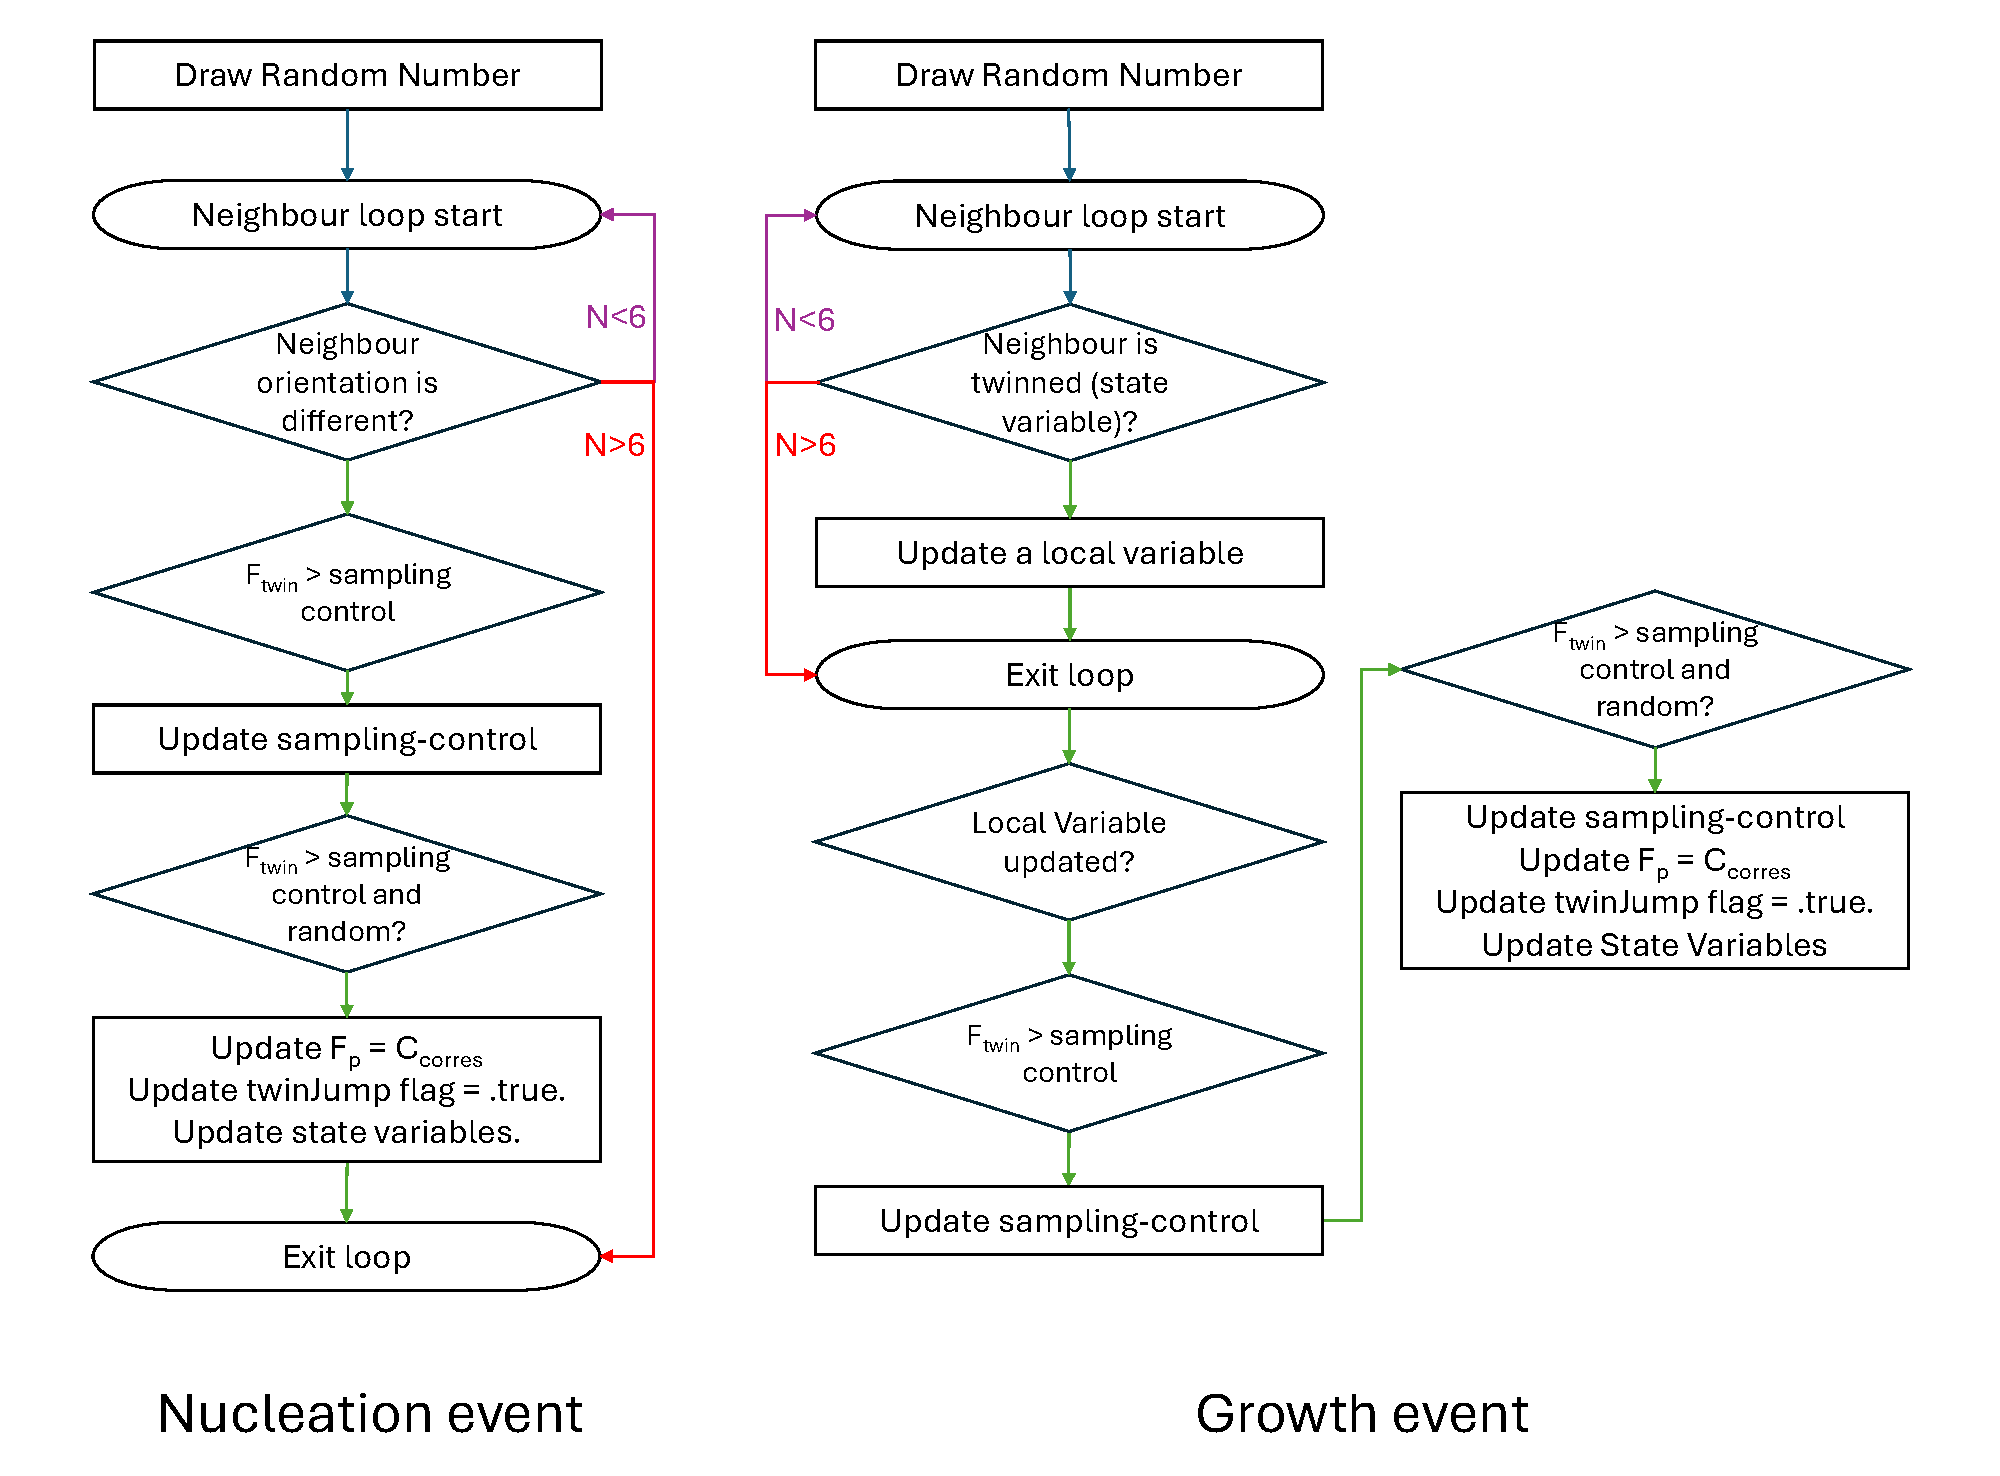
\includegraphics[width=\textwidth]{images/Flow_chart_twin_events.pdf}
    \caption{Initiation of twinning events at a material point.}
    \label{Flow_chart_twin_events}
\end{figure}


\begin{minted}[fontsize=\scriptsize, frame=single]{fortran}
!--------------------------------------------------------------------------------------------
!> @brief calculates instantaneous incremental change of kinematics and associated jump state
!> Satya, Achal
!--------------------------------------------------------------------------------------------
module subroutine plastic_kinematic_deltaFp(ph,en,twinJump,deltaFp)

integer,                     intent(in)  :: &
  ph, &
  en
logical,                     intent(out) :: &
  twinJump
real(pREAL), dimension(3,3), intent(out) :: &
  deltaFp  
integer :: &
  n, &                                               ! neighbor index
  neighbor_e, &                                      ! element index of my neighbor
  neighbor_ip, &                                     ! integration point index of my neighbor
  neighbor_en, &
  neighbor_ph
real(pREAL) :: &
  random, random_g, &
  nRealNeighbors
integer :: &
  twin_var, var_growth
real(pREAL), dimension(param(ph)%sum_N_tw)  :: &
  fdot_twin
real(pREAL), dimension(param(ph)%sum_N_tw)  :: &
  tau_tw
integer :: i

twinJump = .false.
deltaFp = math_I3
  
associate(prm => param(ph), stt => state(ph), dlt => deltastate(ph))
  twin_var = maxloc(stt%f_twin(:,en),dim=1)

  Discrete_twin: if ( prm%discrete_twin ) then
  Frozen: if(stt%frozen(en)<1.0_pREAL) then
    
  call random_number(random)
  call random_number(random_g)
    
  do n = 1, ncellneighbors
    neighbor_e = geom(ph)%IPneighborhood(1,n,en)                   !< Identify neighbor
    !< Identify grain boundary elements
    if (any(dNeq(phase_O_0(ph)%data(en)%asQuaternion(),&
        phase_O_0(ph)%data(neighbor_e)%asQuaternion()))) then       
      Ability_Nucleation: if(stt%f_twin(twin_var,en)> &
                            (stt%fmc_twin(twin_var,en)+ &
                            prm%checkstep(twin_var))) then          !< Frequency control
        stt%fmc_twin(twin_var,en) = stt%fmc_twin(twin_var,en) &
                                  +prm%checkstep(twin_var)
        Success_Nucleation: if (random <= stt%f_twin(twin_var,en)) then          
          twinJump = .true.
          deltaFp  = prm%CorrespondenceMatrix(:,:,twin_var)
          exit
        endif Success_Nucleation
      endif Ability_Nucleation
    endif
  end do

  NeighborLoop: do n = 1, ncellneighbors
    neighbor_e = geom(ph)%IPneighborhood(1,n,en)
    if(stt%variant_twin(neighbor_e)>0) then                    !< Check if neighbor is twinned
      var_growth = stt%variant_twin(neighbor_e)
      exit NeighborLoop
    endif
  enddo NeighborLoop

  Growth_Criteria: if(var_growth>0.0_pReal) then                     !< If neighbor twinned,
    Ability_Growth: if(stt%f_twin(twin_var,en) &
                       >(stt%fmc_twin(twin_var,en) &
                          +prm%checkstep(twin_var))) then            !< Frequency control
      stt%fmc_twin(twin_var,en) = stt%fmc_twin(twin_var,en) &
                                  +prm%checkstep(twin_var)
      Success_Growth: if (0.3_pREAL+random_g*0.7_pREAL 
                           <= stt%f_twin(twin_var,en)) then          !< Random sampling
        twinJump = .true.                                            !< Output flag
        deltaFp  = prm%CorrespondenceMatrix(:,:,twin_var)            !< Correspondence Matrix
      endif Success_Growth
    endif Ability_Growth
  endif Growth_Criteria
  
  endif Frozen
  end if Discrete_twin
end associate
  
end subroutine plastic_kinematic_deltaFp
\end{minted}


\section{Handling of twinning and slip in the kinematics.}

\subsection{Consequences of a “Success” event in Sampling Outcome:}
The impacts of Monte-Carlo “success” are equivalent for nucleation and growth, triggering a flip from the parent to the twinned state. This transformation follows the correspondence matrix formulation discussed earlier. The matrix combines the twinning shear (S) and lattice rotation (U) of mechanical twinning.

\subsection{The Twinning Jump.}
The primary consequence of a parent-to-twin flip is a sudden jump in the plastic deformation gradient Fp, arising from twinning-induced rotation and shear. This contrasts the typical gradual Fp rate evolution from crystal plasticity dislocation slip, as shown in Figure \ref{fig: Kinematic_jump}.
\begin{figure}[H]
    \centering
    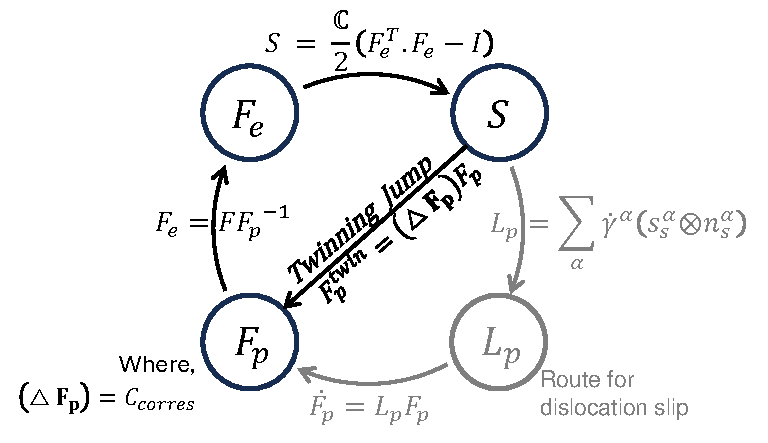
\includegraphics[width=0.7\textwidth]{images/Kinematic_Jump.pdf}
    \caption{Twinning kinematic framework.}
    \label{fig: Kinematic_jump}
\end{figure}
\subsubsection{The ``delta state".}
It is necessary to express the change in the state in terms of an instantaneous jump rather as rate of change. Here we device a rate independent constitutive description.
We treat deformation twinning as a instantaneous jump and in the DAMASK the variables related to deformation twinning are undated in the ``delta state".

We use 4 delta state variables which defines the micro structure parameters.
\begin{enumerate}
    \item f\_twin : Variable used for the random sampling criteria.
    \item fmc\_twin : Variable used for the sampling frequency control.
    \item frozen or f\_binary \\ Discrete quantity which assumes either +1 or -1. It is also used to freeze the voxel so that it is not available for deformation by slip or twinning.
    \item variant\_twin : Used to store the variant of the twin.
\end{enumerate}

\begin{minted}[fontsize=\scriptsize, frame=single]{fortran}
!-------------------------------------------------------------------
!> @brief calculates (instantaneous) incremental change of 
!> microstructure
!> Satya, Achal
!-------------------------------------------------------------------
module subroutine plastic_phenopowerlaw_deltaState(ph,en)
  implicit none
  integer, intent(in)::&
    ph, &
    en
  logical :: &
    twinJump
  integer :: &
    twin_var
  real(pREAL), dimension(3,3) :: &
    deltaFp
    
  associate(prm => param(ph), stt => state(ph), dlt => deltastate(ph))
    twin_var = maxloc(stt%f_twin(:,en),dim=1)
    call plastic_kinematic_deltaFp(ph,en,twinJump,deltaFp)
      if(twinJump) then
        dlt%f_twin(:,en)     = 0.0_pReal - stt%f_twin(:,en)
        dlt%fmc_twin(:,en)   = 0.0_pReal - stt%fmc_twin(:,en)
        dlt%frozen(en)       = 1.0_pReal - stt%frozen(en)
        dlt%variant_twin(en) = twin_var 
      else
        dlt%f_twin(:,en)     = 0.0_pReal
        dlt%fmc_twin(:,en)   = 0.0_pReal
        dlt%frozen(en)       = 0.0_pReal
        dlt%variant_twin(en) = 0.0_pREAL
      endif
  end associate
  
  end subroutine plastic_phenopowerlaw_deltaState
\end{minted}

The delta state variables which sits at the end of the global container will update the state variable at the given time step explicitly.

\subsection{Correspondence matrix.}
\begin{wrapfigure}{rH}{0.35\textwidth}
    \centering 
    \resizebox{0.35\textwidth}{!}{
    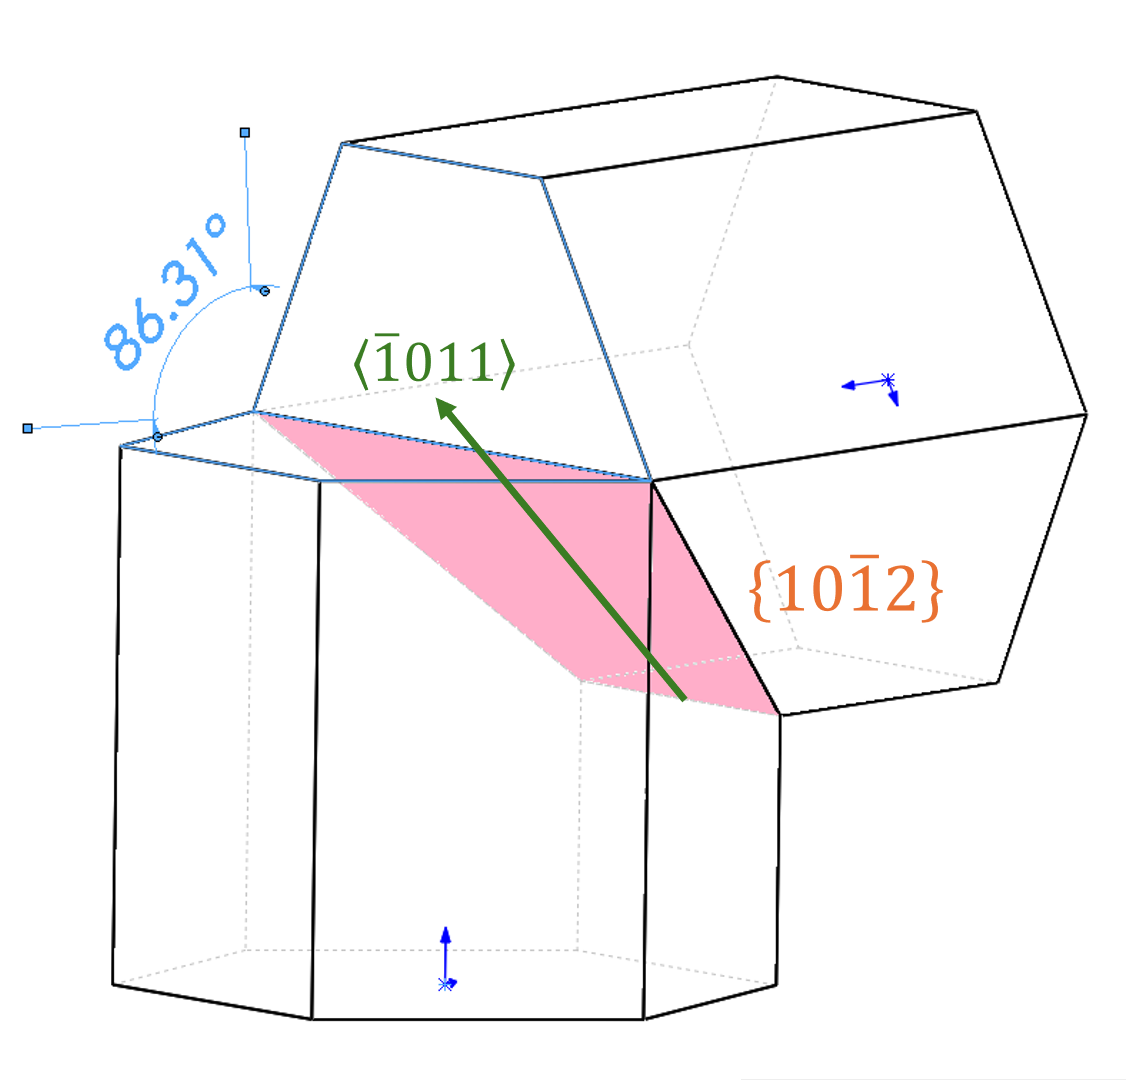
\includegraphics[width=0.5\textwidth]{images/Extension_twin_crystallography.png}}
    \caption{Extension twin crystallography replicated using 3D CAD model in \textbf{SolidWorks}.}
    \label{Extension twin crystallography}
\end{wrapfigure}

When twinning occurs, the parent crystal is sheared and reoriented. The misorientation in two lattices is the unique for a particular twinning mode. For example, $(\bar{1}012)[10\bar{1}1]$ twinning mode in Mg with c/a ratio 1.624 can be recognized by the unique misorientation of 86.31 degrees angle between c-axis in the parent and twin.

This is shown in the figure \ref{Extension twin crystallography} where we take 2 hexagonal lattices with c/a ratio of 1.624 in a CAD software like \textbf{Solidworks}. We then cut it in $(\bar{1}012)$ plane and assemble the lattices in $[10\bar{1}1]$ direction and measure the angle between the corresponding faces of parent and twin. The measured angle gives the unique misorientation angle which is 86.31 degrees.

This crystallographic transformation is mathematically described by the correspondence matrix given by Niewczas \cite{Niewczas121}. Correspondence matrix gives equation for transformation of vector or a plane in parent lattice to twinned lattice. Correspondence matrix provides essential means to predict the physical transformation of crystallographic directions and planes resulting from twinning. Appendix \ref{Appendix:Correspondence_matrix} has more details about the correspondence matrix approach.

\subsection{Incorporating Large deformation caused by Twinning.}

\begin{figure}[H]
    \centering
    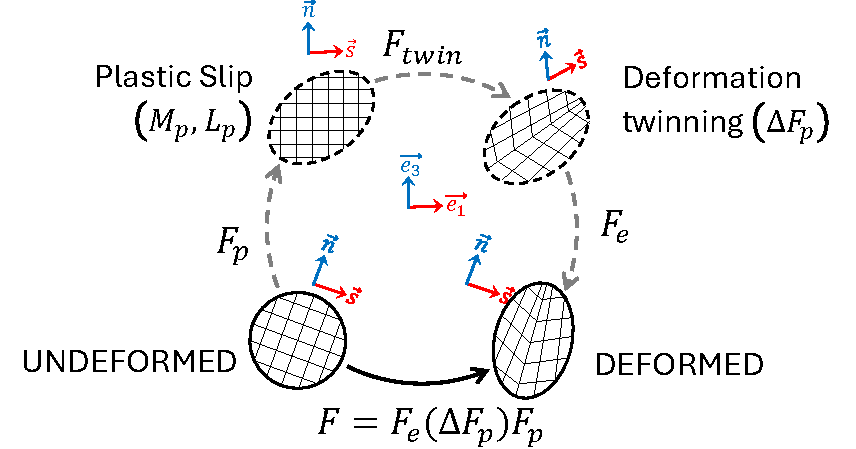
\includegraphics[width=0.55\textwidth]{images/Delta_twin_as_Intermediate_configuration.pdf}
    \caption{Delta State of Twinning as intermediate configuration.}
    \caption*{\ \ Taking ${F_p}_{(t=0)} = O_0$ so that lattice coordinates $\hat{n}$,$\hat{s}$ coincide with lab coordinate system $\overrightarrow{e_3}$,$\overrightarrow{e_1}$ }
    \label{fig:DeltaStateIntermediateConfig}
\end{figure}

In the single constituent kinematics, clear distinction is made between different deformation modes: Elastic deformation and Plastic Deformation and within the plastic deformation modes: Slip and Twinning. Twinning which causes sudden change in the shear and it reorients the lattice. Hence, is not evaluated along with the slip but it is pre-multiplied to the plastic deformation gradient. The above figure \ref{fig:DeltaStateIntermediateConfig} shows how both the shear and reorientation are introduced in the lattice.

\begin{figure}[H]
    \centering
    \fbox{\resizebox{0.6\textwidth}{!}{
    \begin{circuitikz}
\tikzstyle{every node}=[font=\LARGE]
\draw  (22.5,30.5) rectangle (30,21.75);
\draw [short] (23.75,30.5) -- (23.75,21.75);
\draw [short] (25,30.5) -- (25,21.75);
\draw [short] (26.25,30.5) -- (26.25,21.75);
\draw [short] (27.5,30.5) -- (27.5,21.75);
\draw [short] (28.75,30.5) -- (28.75,21.75);
\draw [short] (22.5,29.25) -- (30,29.25);
\draw [short] (22.5,28) -- (30,28);
\draw [short] (22.5,26.75) -- (30,26.75);
\draw [short] (22.5,25.5) -- (30,25.5);
\draw [short] (22.5,24.25) -- (30,24.25);
\draw [short] (22.5,23) -- (30,23);

% Sheared config

\draw [short] (21.25,8) -- (22.5,16.75);
\draw [short] (21.25,8) -- (28.75,8);
\draw [short] (28.75,8) -- (30,16.75);
\draw [short] (22.5,16.75) -- (30,16.75);

\draw [short] (22.33,15.5) -- (29.83,15.5);
\draw [short] (22.15,14.25) -- (29.65,14.25);
\draw [short] (21.97,13) -- (29.47,13);
\draw [short] (21.79,11.75) -- (29.29,11.75);
\draw [short] (21.61,10.5) -- (29.11,10.5);
\draw [short] (21.43,9.25) -- (28.93,9.25);

\draw [short] (22.5,16.75) -- (22.5,8);
\draw [short] (23.75,16.75) -- (23.75,8);
\draw [short] (25,16.75) -- (25,8);
\draw [short] (26.25,16.75) -- (26.25,8);
\draw [short] (27.5,16.75) -- (27.5,8);
\draw [short] (28.75,16.75) -- (28.75,8);

%Twinned config

\draw [short] (40,16.75) -- (47.5,16.75);
\draw [short] (36.25,8) -- (43.75,8);
\draw [short] (39.4,15.5) -- (46.9,15.5);
\draw [short] (38.75,14.25) -- (46.25,14.25); 
\draw [short] (36.9,9.25) -- (44.4,9.25);
\draw [short] (37.5,10.5) -- (45,10.5);

\draw [short] (46.25,16.75) -- (46.25,14.25);
\draw [short] (45,16.75) -- (45,14.25);
\draw [short] (43.75,16.75) -- (43.75,14.25);
\draw [short] (42.5,16.75) -- (42.5,14.25);
\draw [short] (41.25,16.75) -- (41.25,14.25);
\draw [short] (40,16.75) -- (40,14.25);
%\draw [short] (38.75,16.75) -- (38.75,14.25);
\draw [short] (43.75,10.5) -- (43.75,8);
\draw [short] (42.5,10.5) -- (42.5,8);
\draw [short] (41.25,10.5) -- (41.25,8);
\draw [short] (40,10.5) -- (40,8);
\draw [short] (38.75,10.5) -- (38.75,8);
\draw [short] (37.5,10.5) -- (37.5,8);
%\draw [short] (36.25,10.5) -- (36.25,8);


\draw [short] (43.75,10.5) -- (45,14.25);
\draw [short] (42.5,10.5) -- (43.75,14.25);
\draw [short] (41.25,10.5) -- (42.5,14.25);
\draw [short] (40,10.5) -- (41.25,14.25);
\draw [short] (38.75,10.5) -- (40,14.25);
\draw [short] (37.5,10.5) -- (38.75,14.25); % left edge y = 3 x - 102
%\draw [short] (36.25,10.5) -- (37.5,14.25);
\draw [short] (45,10.5) -- (46.25,14.25); % right edge y = 3 x - 124.5

\draw [short] (38.625,13.875) -- (45.375,11.625); %x = 45.375 and y = 11.625, x = 38.625 and y = 13.875
\draw [short] (41.25,14.25) -- (45.75,12.75); % x = 45.75 and y = 12.75
\draw [short] (45,14.25) -- (46.125,13.875); % x = 46.125 and y = 13.875
\draw [short] (38.25,12.75) -- (45,10.5); % x = 38.25 and y = 12.75
\draw [short] (37.875,11.625) -- (41.25,10.5); %x = 37.875 and y = 11.625

\draw [short] (43.75,8) -- (45,10.5);
\draw [short] (46.25,14.25) -- (47.5,16.75);
\draw [short] (36.25,8) -- (37.5,10.5);
\draw [short] (38.75,14.25) -- (40,16.75);


%Final config

\draw [short] (38.022,28.218) -- (39.000,30.500); % left vertical
\draw [short] (36.708,21.985) -- (45.458,23.208); % bottom horizontal
\draw [short] (39.000,30.500) -- (47.750,31.750);  % top
\draw [short] (46.772,29.468) -- (47.750,31.750); % right
\draw [short] (45.947,24.350) -- (37.191,23.099); % 
\draw [short] (46.437,25.491) -- (37.687,24.241); % bottom 2
\draw [short] (38.511,29.359) -- (47.261,30.609); % 
\draw [short] (38.022,28.218) -- (46.772,29.468); %top 2

\draw [short] (37.687,24.241) -- (36.708,21.985);%
\draw [short] (39.145,24.449) -- (38.167,22.167);% bott
\draw [short] (40.603,24.658) -- (39.625,22.375);%
\draw [short] (42.062,24.866) -- (41.083,22.583); % 
\draw [short] (43.520,25.074) -- (42.542,22.792); % 
\draw [short] (44.978,25.283) -- (44.0,23);
\draw [short] (46.437,25.491) -- (45.458,23.208);

\draw [short] (39.480,28.426) -- (40.458,30.708);
\draw [short] (40.939,28.634) -- (41.917,30.917);
\draw [short] (42.397,28.843) -- (43.375,31.125); % tops
\draw [short] (43.855,29.051) -- (44.833,31.333);
\draw [short] (45.313,29.259) -- (46.292,31.542);

\draw [short] (37.687,24.241) -- (38.022,28.218); %Twin
\draw [short] (39.145,24.449) -- (39.480,28.426); %2
\draw [short] (40.603,24.658) -- (40.939,28.634); %3
\draw [short] (42.062,24.866) -- (42.397,28.843);
\draw [short] (43.520,25.074) -- (43.855,29.051);
\draw [short] (44.978,25.283) -- (45.313,29.259);
\draw [short] (46.437,25.491) -- (46.772,29.468);

\draw [short] (45.313,29.259) -- (46.687,28.466);
\draw [short] (43.855,29.051) -- (46.604,27.474);
\draw [short] (42.397,28.843) -- (46.520,26.483);
\draw [short] (40.939,28.634) -- (46.437,25.491);
\draw [short] (39.480,28.426) -- (44.978,25.283);
\draw [short] (38.022,28.218) -- (43.520,25.074);
\draw [short] (37.939,27.226) -- (42.062,24.866);
\draw [short] (37.855,26.235) -- (40.603,24.658);
\draw [short] (37.772,25.243) -- (39.145,24.449);


%Explanation

\draw [->, >=Stealth] (25.75,20.75) -- (25.75,18);
\draw [->, >=Stealth] (32,12.25) -- (34.5,12.25);
\draw [->, >=Stealth] (43.5,18.25) -- (43.5,21.25);
\draw [line width=1.2pt, ->, >=Stealth] (33.25,26.5) .. controls (34.25,27) and (35,27.25) .. (36.25,26.5) ;
\node [font=\Huge] at (26.5,19.5) {$F_p$};
\node [font=\Huge] at (33,13) {$(\Delta F_p)F_p$};
\node [font=\Huge] at (46,19.5) {$F_e(\Delta F_p)F_p$};
\node [font=\Huge] at (34.75,27.5) {$F = F_e(\Delta F_p)F_p$};
\node [font=\Huge] at (25.5,31.5) {\textbf{Reference Configuration}};
\node [font=\Huge] at (40,31.5) {\textbf{Current Configuration}};
\node [font=\Huge] at (41.5,7) {\textbf{Intermediate Configuration,}};
\node [font=\Huge] at (41.5,6) {\textbf{Slip + Twin}};
\node [font=\Huge] at (26.5,7) {\textbf{Intermediate Configuration,}};
\node [font=\Huge] at (26.5,6) {\textbf{Slip}};


\end{circuitikz}}}
    \caption{Multiplication of correspondence matrix to deformation gradient.}
    \label{fig:Twinning kinematics}
\end{figure}

Twinning can be considered as a intermediate configuration in the route drawn from the deformed to unreformed configurations. The figure \ref{fig:Twinning kinematics} shows the route in the single constituent kinematics from deformed to un-deformed configuration.

DAMASK has an intrinsic algorithm for the numerical integration of kinematic quantities $L_p$ \& $L_i$ at a fixed internal material state. The time integration is done implicitly, where solution scheme is implemented by two-level predictor-corrector scheme based on minimizing the residuals $R_i$ and $R_p$. The residual equations are solved by Newton-Raphson scheme where convergence is satisfied when residuals drops below a tolerance limit $\epsilon_i$ and $\epsilon_p$. This algorithm \ref{alg:myalgorithm} is given below .

\begin{algorithm}[H]
\caption{Algorithm for time integration of kinematic variables}
\label{alg:myalgorithm}
\SetKwInOut{Data}{Data}
\SetKwInOut{Result}{Result}
\SetKwInOut{Initialization}{Initialization}
\SetKwRepeat{DoWhile}{do}{while}
\SetKwFor{While}{while}{do}{end}
\SetKwFor{Loop}{loop}{do}{end}

\Data{$[F]_{t_n}, [F_p]_{t_{n-1}}, [F_i]_{t_{n-1}}$}
\Result{$y = x^n$}

\Initialization{
  $\tilde{[L_p]}_{t_n}^0 = [L_p]_{t_{n-1}}$\;
  $\tilde{[L_i]}_{t_n}^0 = [L_i]_{t_{n-1}}$\;
  $j = 1$\;
}

\While{$\|R_i\| \geq \epsilon_i$}{
  $[F_i]_{t_n} = (I - \Delta t \tilde{[L_i]}_{t_n}^{j-1})^{-1} [F_i]_{t_{n-1}}$\;
  $k = 1$\;
  
  \Loop{$\|R_p\| \geq \epsilon_p$}{
    $[F_p]_{t_n} = (I - \Delta t \tilde{[L_p]}_{t_n}^{k-1})^{-1} [F_p]_{t_{n-1}}$\;
    $[F_e]_{t_n} = [F]_{t_n} [F_p^{-1}]_{t_n} [F_i^{-1}]_{t_n}$\;
    $[S]_{t_n} = f([F_e]_{t_n}, [F_e]_{t_n})$\;
    $R_p = \tilde{[L_p]}_{t_n}^{k-1} - L_p([S]_{t_n}, [F_i]_{t_n})$\;
    $\tilde{[L_p]}_{t_n}^{k} = \tilde{[L_p]}_{t_n}^{k-1} - \alpha_p \left(\frac{\partial \tilde{R_p}}{\partial [L_p]}\right)^{-1} R_p$\;
    $k = k + 1$\;
  }
  
  $R_i = \tilde{[L_i]}_{t_n}^{j-1} - L_i([S]_{t_n}, [F_i]_{t_n})$\;
  $\tilde{[L_i]}_{t_n}^{j-1} = \tilde{[L_i]}_{t_n}^{j-1} - \alpha_i \left(\frac{\partial \tilde{R_i}}{\partial [L_i]}\right)^{-1} R_i$\;
  $j = j + 1$\;
}

\end{algorithm}


For implementation of deformation caused by twinning in the DAMASK source code, the subroutine ``plastic\_kinematicJump" is called from the phase\_mechanical module of DAMASK. A logical flag carries the result from random sampling. If it carries a ``success" the $F_{p0}$ is updated in the phase\_mechanical\_constitutive function as follows:

\begin{minted}[fontsize=\scriptsize, frame=single]{fortran}
Fp0 = matmul(deltaFp,phase_mechanical_Fp0(ph)%data(1:3,1:3,en))
\end{minted}

In addition to this state must be updated to reflect the changes made by delta state due to twinning and the updated state should also be preserved for next iteration as follows:
\begin{minted}[fontsize=\scriptsize, frame=single]{fortran}
o = plasticState(ph)%offsetDeltaState
sd = plasticState(ph)%sizeDeltaState
      
!update current state by jump
plasticState(ph)%state(o+1:o+sd,en) = plasticState(ph)%state(o+1:o+sd,en) & 
                                     + plasticState(ph)%deltaState(o+1:o+sd,en)
      
!store jumped state as initial value for next iteration
state0(o+1:o+sd) = plasticState(ph)%state(o+1:o+sd,en)
\end{minted}

The elements adjacent to the twinned element will experience large shear and the neighbouring elements may also twin in the next iterations until it stop at obstacles like grain boundary. So, it is necessary to circumvent the loops calculating $L_p$ and $L_i$ in the current iteration. This is done modifying the below statements.

\begin{minted}[fontsize=\scriptsize, frame=single]{fortran}
!converged if below absolute tolerance or upon twinJump
elseif (norm2(residuumLp) < atol_Lp .or. twinJump) then      
    exit LpLoop
\end{minted}

\begin{minted}[fontsize=\scriptsize, frame=single]{fortran}
!converged if below absolute tolerance or upon twinJump
elseif (norm2(residuumLi) < atol_Li .or. twinJump) then      
    exit LiLoop
\end{minted}

The outermost state loop is bypassed by setting the todo flag as false in the \\ phase\_mechanical\_constitutive function.
\begin{minted}[fontsize=\scriptsize, frame=single]{fortran}
if(twinJump) then
    todo = .false.
\end{minted}



\chapter{Model Study.}
The development process of any constitutive model involves testing of the individual components which make up the model.

\begin{wrapfigure}{r}{0.45\textwidth}
 \includegraphics[width=0.45\textwidth]{images/Result_correspondence_matrix.pdf}
 \caption{Testing the Correspondence Matrix subroutine.}
  \label{Correspondence_matrix_program}
\end{wrapfigure}



Model study can be further divided into ``component testing" where we test individual components of the model and ``model testing" where we test the entire model.

\section{Model Component testing}

\subsection{Testing Correspondence Matrix subroutine.}

The subroutine for generating the correspondence matrix was written inside the framework of the DAMASK. It utilizes many intrinsic components within the DAMASK such as:

\begin{itemize}
    \item Schmid Matrix.
    \item Generation of Normal Vector and Direction vector for different twin system
    \item Generation of Characteristic Shear for different twinning modes and also for different c/a ratios.
\end{itemize}

A new function was also introduced. This function generates the re-indexation matrix from the normal vector.

The correspondence matrix subroutine generates the correspondence matrix for different types of twins and HCP metals with different c/a ratios.

The complete program to generate the correspondence matrix is given in Appendix \ref{Appendix:Correspondence_matrix}

The figure \ref{Correspondence_matrix_program} is the result from the program used to generate the correspondence matrix.


\subsection{Testing the reorientation in the deformation kinematics.}
The multiplicative decomposition is done such that the current crystallographic orientation $O$ can then always be calculated from elastic deformation gradient $F_e$ through a polar decomposition 
\begin{equation*}
    F_e = O^T U
\end{equation*}
 where $U$ is the right stretch tensor.

 We use this result to verify that the pre-multiplication of correspondence matrix will result in the reorientation of twinned lattice in the single constituent kinematics formulation of the DAMASK.
\subsubsection{Brief summary of the code to test reorientation:}
First, the code defines parameters such as twin direction, habit plane normal, material properties, and initial Euler angles. These values are then used to calculate the norm of the twin direction and plane normal, unit vectors, and characteristic shear for extension twinning. The initial orientation of the crystal is defined using Euler angles. The twinning operation is applied by multiplying the deformation gradient with the correspondence matrix. Polar decomposition of the final deformation gradient is performed to separate the rotation and stretching components. Finally, the code calculates the disorientation angle between the initial and final crystal orientations, which quantifies the amount of rotation caused by twinning.

 The verification is done using a python script given in Appendix \ref{Appendix:Correspondence_matrix}. The figure \ref{Reorientation_test} shows the result of the python script.

 \begin{figure}[H]
    \centering
    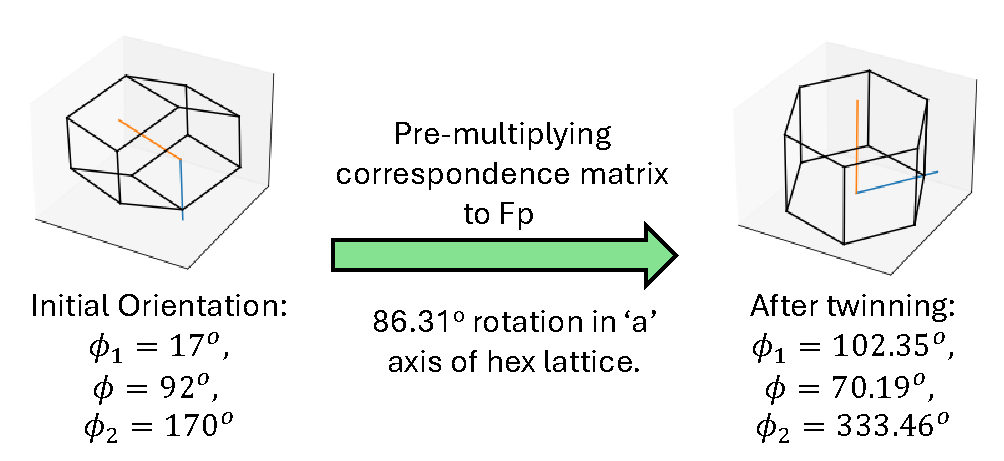
\includegraphics[width=0.7\textwidth]{images/Reorientation_Test.pdf}
    \caption{Reorientation test.}
    \label{Reorientation_test}
 \end{figure}

\section{Model Testing}

For testing the entire model, it is necessary to run a complete DAMASK simulation. In this section DAMASK simulation workflow is briefly discussed.

\subsection{The DAMASK simulation procedure.}

A typical DAMASK simulation procedure consist of preprocessing tasks to create the input files for running the simulation and postprocessing tasks to read and analyze the output file from the simulation.

Figure \ref{DAMASK_workflow} shows the DAMASK simulation procedure.

\begin{figure}[H]
    \centering
    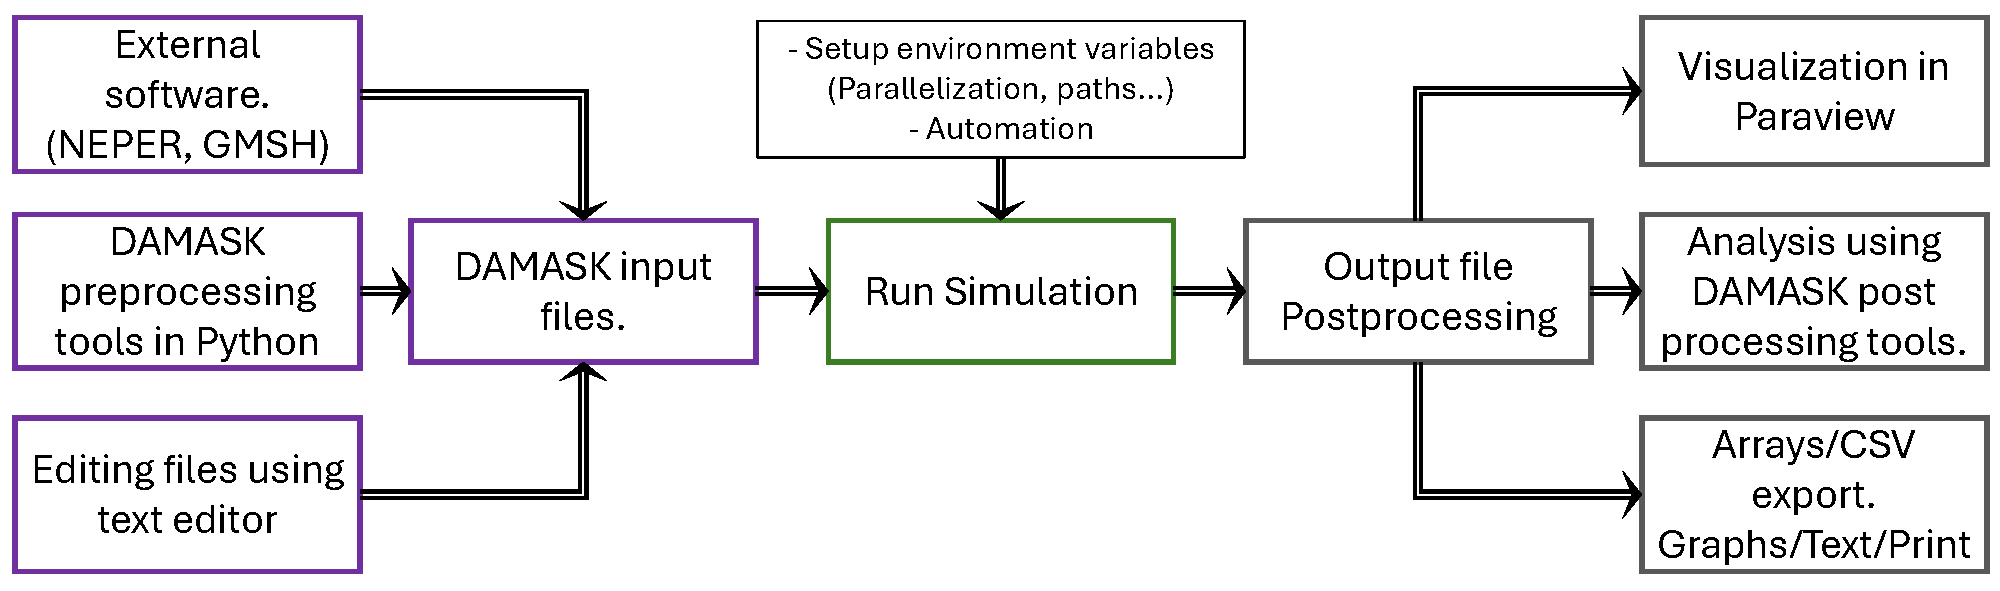
\includegraphics[width=\textwidth]{images/DAMASK_workflow.pdf}
    \caption{Flow chart of DAMASK Simulation Procedure.}
    \label{DAMASK_workflow}
\end{figure}

\subsubsection{Preprocessing}
Preprocessing involves generation of 3 input files:
\begin{enumerate}
\item Geometry file (*.vti for FFT solver or *.msh for FEM solver) \\ Geomtery file has the details of the Representative Volume Element(RVE) which contains the details about grain size, shape, volume etc.\\
Geometry file can be generated using DAMASK preprocessing tools in Python or using external software like NEPER or GMSH.
\item \{Material\}.yaml file: \\ Material file has the details of microstructural parameters like elastic constants, lattice parameters, the orientation of each grain in the RVE. It also has details about the constitutive law used and the parameters used in the constitutive law like slip parameters, twin parameters, etc. \\
\{Material\}.yaml file can be generated using DAMASK preprocessing tools, it can also be edited using a text editor.
\item \{Load\}.yaml file: \\ Load file has the details of boundary conditions and discretization which can be given in steps.
The displacement boundary condition can be defined in terms of $\Dot{F}$ or $L$ or $F$ (rate of deformation gradient, velocity gradient or deformation gradient) and load boundary condition can be defined in terms on $\Dot{P}$(rate of First-Piola-Kirchoff-Stress) or P (PK1).\\
\{Load\}.yaml file can be generated using DAMASK preprocessing tools and it can be edited using a text editor.
\end{enumerate}

\subsubsection{Simulation}
Before running a simulation the environment can be set for DAMASK by running 
\begin{lstlisting}[language=bash, basicstyle=\small\ttfamily, frame=single]
source ./{DAMASK_source_folder_path}/env/DAMASK.sh
\end{lstlisting}

DAMASK has gives choice between FFT and FEM solvers which are part of DAMASK. Simulations can also be run in MSC MARC solver. For our work we primarily use FFT solver or ``DAMASK\_grid".

\subsubsection{Postprocessing}
The data from the DAMASK simulation will be stored in HDF5 (Hierarchical Data File) file.  Data in the HDF5 output files has to be processed for further analysis or visualization. DAMASK provides postprocessing tools in Python to make manipulate and process the data in HDF5 files.



\subsection{Bycrystal Representative Volume Element.}

For testing our mechanical twinning model, we employ a 2-dimensional bicrystal RVE containing a hard matrix phase and a soft inclusion phase. The hard surrounding crystal or ``matrix" is oriented such that it has a higher critical resolved shear stress for activating twinning, while the soft inclusion is more amenable to mechanical twinning. This offers us simple test case consisting of two grains with a grain boundary. The RVE is of dimension 100$\mu$mx100$\mu$m and it is discretized to 64x64 FFT grid elements. This simple RVE is used to test our discrete twinning model.

\begin{figure}[H]
    \centering
    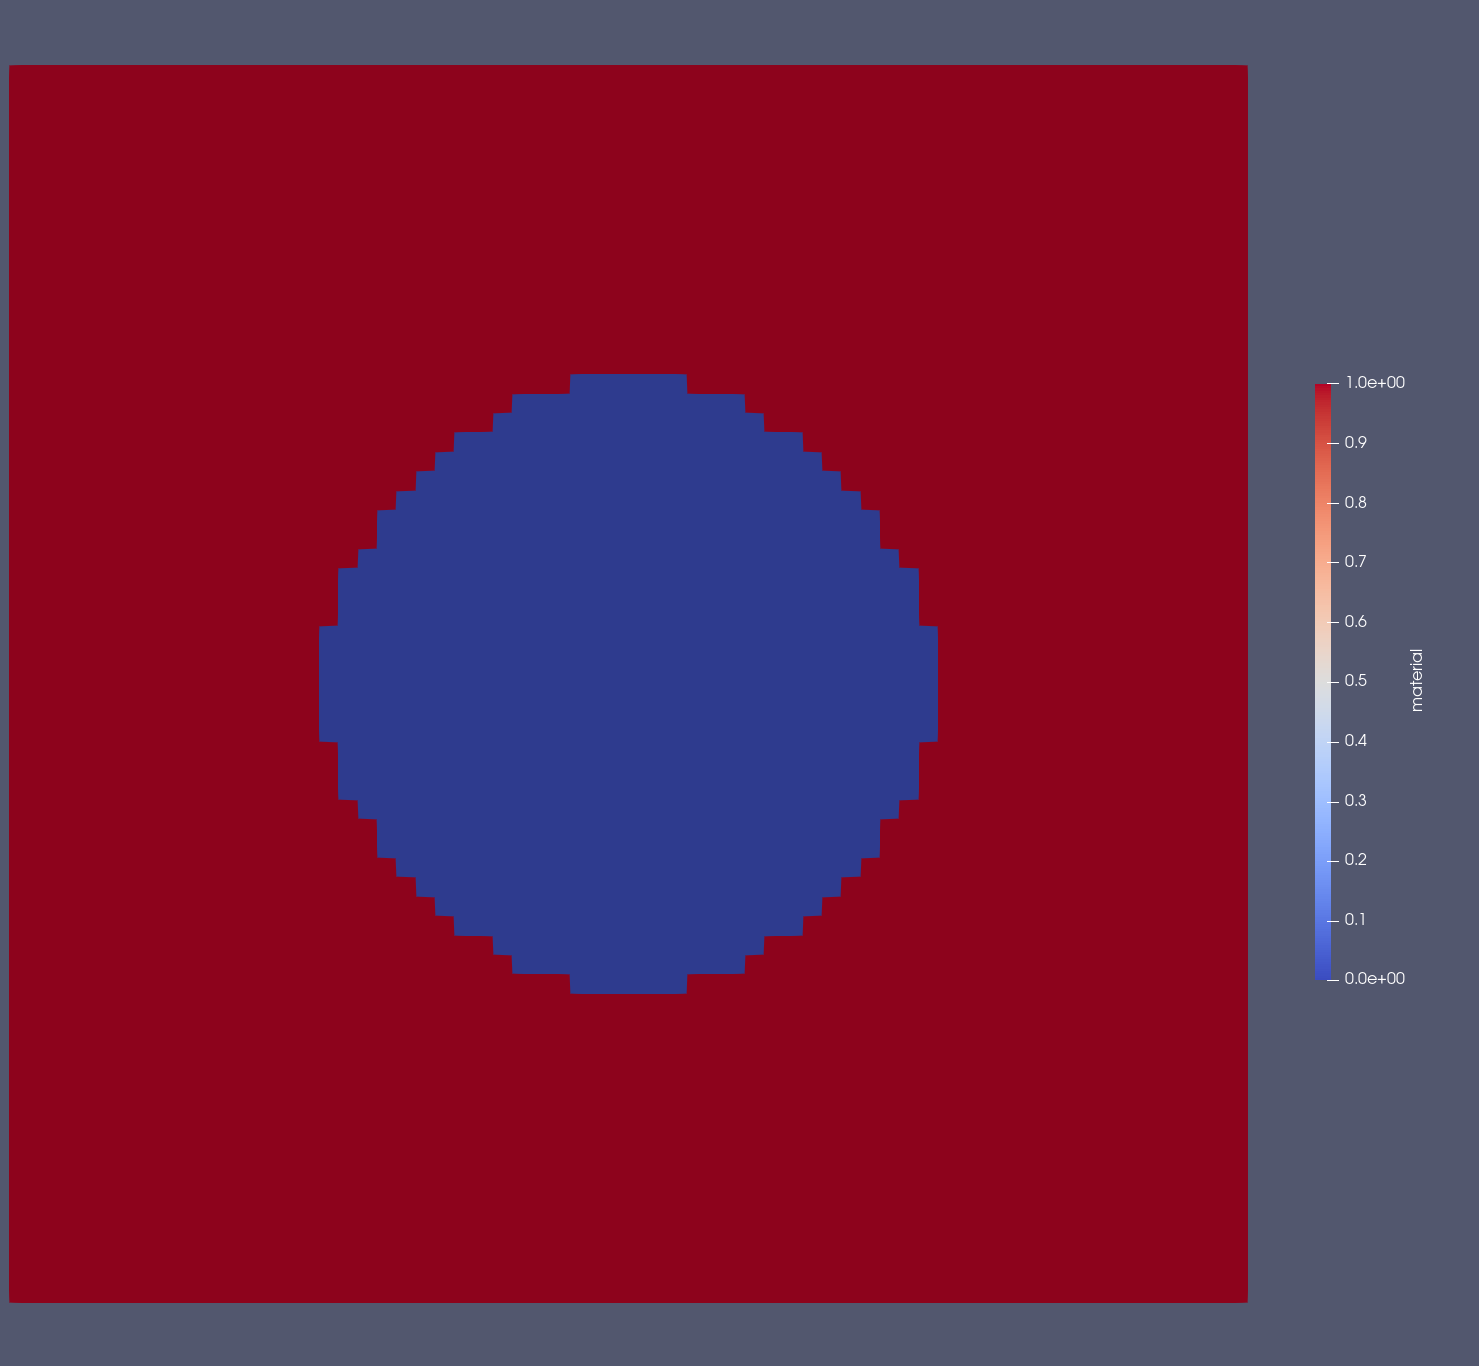
\includegraphics[width=0.4\textwidth]{images/Bycrystal_RVE.png}
    \caption{Bicrystal Representative Volume Element.}
    \label{fig:Bycrystal RVE.}
\end{figure}

%Schmid Factor for twinning

%Boundary Condition
%Boundary condition is given for this test case as:


\subsection{Test for nucleation.}

\begin{figure}[H]
    \centering
    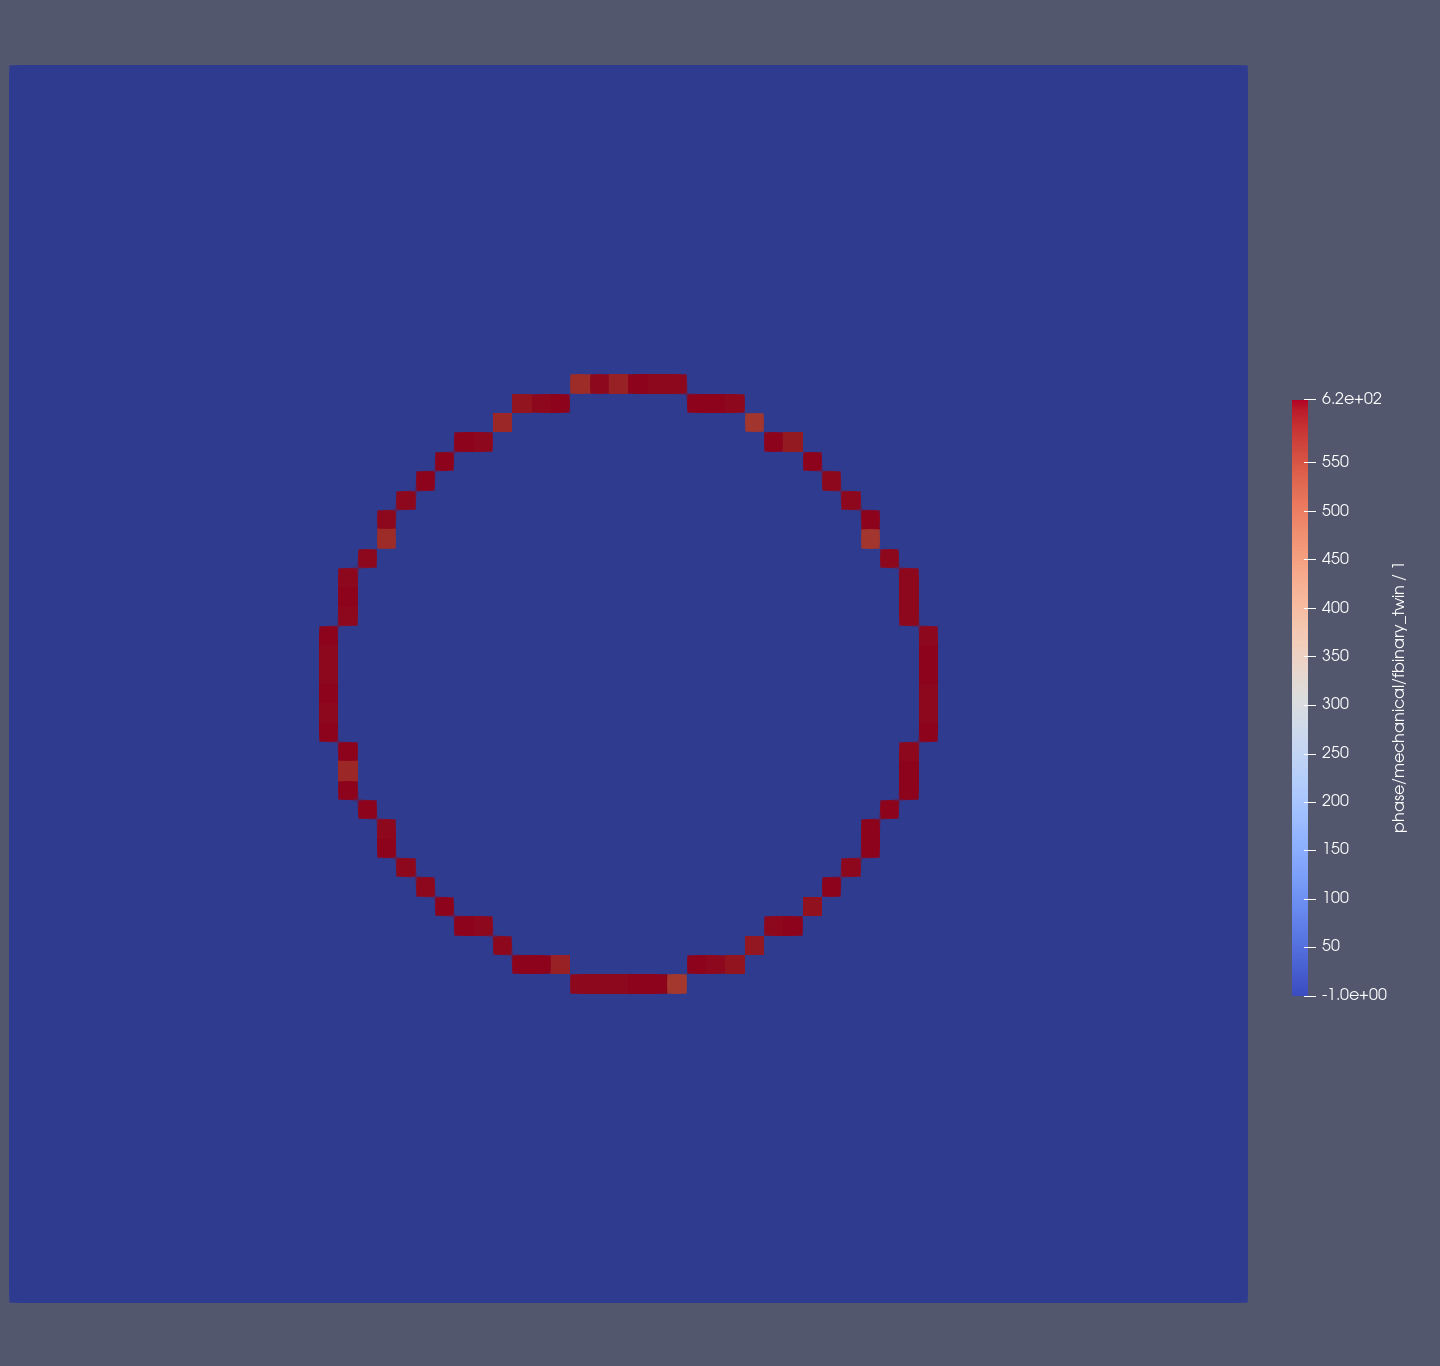
\includegraphics[width=0.4\textwidth]{images/Grain boundray identification test.png}
    \caption{Selection of grain boundary elements for nucleation.}
    \label{fig:Selection of grain boundary elements.}
\end{figure}

The nucleation of the twins are assumed to occur at the grain boundaries. Grain boundary is the surface at which single crystals having different orientations meet each other. The nucleation code identifies the neighbours and if the two neighbouring elements have different orientations, then we consider the elements to be at the grain boundary. Grain boundary elements are sampled for nucleation. We take a bicrystal RVE to test the nucleation.

The figure \ref{fig:Selection of grain boundary elements.} shows the bicrystal RVE which shows the grain boundary elements which are identified as potential nucleation region.

\subsection{Test for growth.}
For testing the growth behavior, we consider the same program used for nucleation in addition with program for growth, as the growth process involves selective random sampling of the neighboring voxels/elements that are adjacent to twinned regions. Therefore, the growth process follows after the nucleation events. To test the growth behavior, we employ a bicrystal representative volume element (RVE). The image below illustrates the growth and band thickening of twins, which propagates from one grain boundary to another grain boundary. In this image the bycrystal RVE is superimposed on the simulation output which shows the variation of the discrete twinning variable "f\_binary"

\begin{figure}[H]
    \centering
    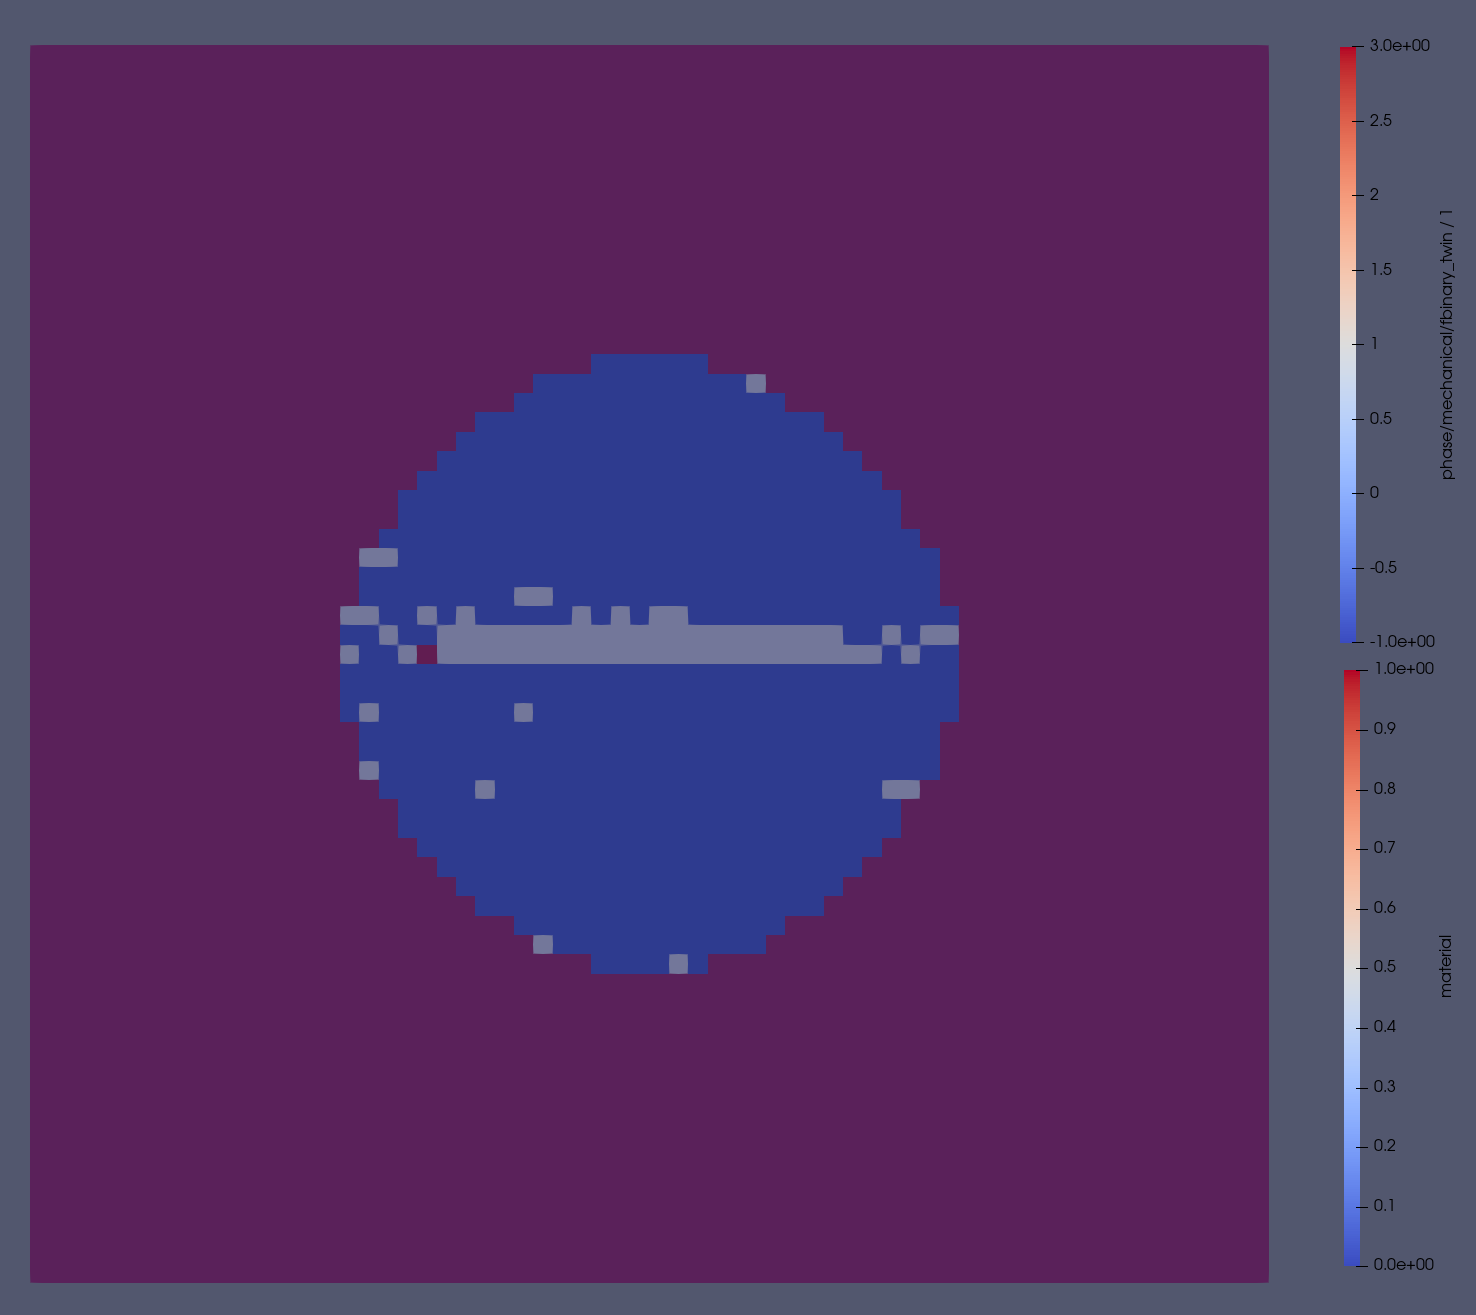
\includegraphics[width=0.4\textwidth]{images/Growth.png}
    \caption{Testing the program for growth.}
    \label{fig:Selection of neighbour elements for growth.}
\end{figure}

%\chapter{Conclusions and discussions.}
%input{}

\chapter{Conclusions and Future Scope.}
\section{Conclusions.}
In the literature, we found statistical studies proving that twinning is an inherently stochastic phenomenon distributed probabilistically across geometrical parameters. Previous deterministic models failed to capture this stochastic nature adequately. We addressed this limitation by modeling the stochasticity in our constitutive law using a random sampling technique inspired by Monte Carlo methods.  For simplicity, we consider the random sampling to be uniformly distributed, and we control the frequency of sampling and the range of random numbers.

\vspace{0.2cm}

Based on experimental observations and results from energy-based modeling approaches, we assume that the nucleation of twins occurs at grain boundaries. We employ selective random sampling at grain boundaries to model the nucleation events, using local stress criteria. For twin growth, which includes propagation and band thickening, we use selective random sampling of neighboring twinned voxels/elements, as a newly nucleated site induces large shear in the neighborhood. The distribution of random numbers and frequency control can be applied separately for nucleation and growth events.

\vspace{0.2cm}

Next, we model twinning as a discrete entity, enabling a spatially resolved representation of twinning events that aligns with experimental observations. This approach allows for more accurate prediction of texture evolution, which volume fraction-based models lack the capability to resolve spatially.

\vspace{0.2cm}

We consider twinning as a ``Jump" rather than a ``pseudo-slip" approach, applying the twinning shear and reorientation directly to the plastic deformation gradient $F_p$. This captures the localized deformation effects of twinning at appropriate time scales. For this, we use the correspondence matrix approach, providing a rigorous crystallographic basis by combining the twinning shear (S) and lattice rotation (U) of mechanical twinning to model the lattice reorientation and deformation associated with twinning.

\vspace{0.2cm}

For implementing our model, we chose DAMASK, an open-source crystal plasticity software that provides the facility to modify constitutive laws and integrate custom formulations due to its modular construction. DAMASK's ability to access internal subroutines facilitated the implementation of our model on a stable platform for testing. We treat twinning as an intermediate configuration with a sudden jump in the plastic deformation gradient $F_p$, departing from the gradual $F_p$ rate evolution associated with dislocation slip in crystal plasticity. This is implemented by modifying the time integration algorithm for kinematic variables in DAMASK and circumventing loops for convergence while updating the plastic deformation gradient.

\vspace{0.2cm}

Our work advances the understanding and modeling of deformation twinning in HCP metals by addressing gaps or limitations identified in the literature, such as the stochastic nature of twinning, accurate spatial resolution of twins, and capturing the localized deformation effects through a crystallographically rigorous approach. This can potentially lead to more accurate predictions of texture evolution and deformation behavior in HCP metals, enabling better material design and performance optimization.

\section{Future scope: Full Scale Model Testing.}
For publication of the discrete twinning constitutive model it is necessary to test it against other models and with experiments. We need to run simulations for 3D polycrystal Representative Volume Elements (RVEs) for running these tests. Here we discuss the process of model testing.

\subsection{Benchmark the simulations.}

Before running polycrystal simulations to test our code, it is essential to benchmark the simulation results against known solutions or experimental data. This process involves running a set of pre-processing codes with well-understood material parameters and boundary conditions and comparing the simulation results with established benchmarks. For this purpose, we have chosen to benchmark our simulations against the results of Wang et al. (2014) \cite{WANG201477}, where simulations were performed on pure magnesium using the DAMASK software, and the results were compared with experimental observations.

Benchmarking against a reliable source serves several purposes:

\begin{enumerate}
    \item Verification: It verifies the correct implementation of the constitutive model, numerical algorithms, and boundary conditions within our code.
    \item Validation: It validates the model's ability to reproduce known phenomena and results accurately.
    \item Calibration: It aids in calibrating material parameters and identifying potential discrepancies or sources of error.
    \item Establishing Confidence: Successful benchmarking builds confidence in the reliability and accuracy of our simulation framework before proceeding with further investigations or parametric studies.
\end{enumerate}

\subsection{Benchmark simulation setup.}

Lattice parameters and elastic properties of Mg for the simulation is based on \cite{HULL1922189}  \\ $\{\bar{1} 0 1 2\} \langle 1 0 \bar{1} 1 \rangle$ Extension twin system in Magnesium:

\begin{table}[H]
    \begin{subtable}{0.45\textwidth}
    \centering
    \caption{Crystallography of twinning.}
    \label{tab:Twin_geometry}
        \begin{tabular}{cccc}
        \hline
        $\nu_1$ & $K_1$ & $\nu_2$ & $K_2$ \\
        \hline
        $\langle  \bar{1} 0 1 1 \rangle$ & $\{ 1 0 \bar{1} 2 \}$ & $\langle 1 0 \bar{1} 1 \rangle$ & $\{ 1 0 \bar{1} \bar{2} \}$ \\
        \hline
        \end{tabular}
    \end{subtable}
    \begin{subtable}{0.45\textwidth}
    \centering
    \caption{Lattice parameters.}
    \label{tab:cOverA}
        \begin{tabular}{cccc}
        \hline
        parameter & c & a & c/a \\
        \hline
        value & 1.6235 & 1 & 1.6235 \\
        \hline
        \end{tabular}
    \end{subtable}
    \caption{Crystallography of twinning and lattice parameters.}
    \label{tab:Twin_crystallography}
    
\end{table}



%next subtables should start immediately after previous one else it will not be side by side.
\begin{table}[H]

    \begin{minipage}[h]{0.45\textwidth}
    \begin{subtable}{\textwidth}
    \centering
    \caption{$\langle \Bar{1} 0 1 1 \rangle \{ 1 0 \Bar{1} 2 \}$ extension twin system.}
    \label{tab:Twins1}
        \begin{tabular}{ccc}
            \hline
            index & plane normal & slip direction \\
            \hline
            $V1$ & $(\bar{1} 1 0 2)$ & $[ 1 \bar{1} 0 1]$ \\
            $V2$ & $(1 0 \bar{1} 2)$ & $[ \bar{1} 0 1 1]$ \\
            $V3$ & $(0 \bar{1} 1 2)$ & $[ 0 1 \bar{1} 1]$ \\
            $V4$ & $(1 \bar{1} 0 2)$ & $[ \bar{1} 1 0 1]$ \\
            $V5$ & $(\bar{1} 0 1 2)$ & $[ 1 0 \bar{1} 1]$ \\
            $V6$ & $(0 1 \bar{1} 2)$ & $[ 0 \bar{1} 1 1]$ \\
            \hline
        \end{tabular}
    \end{subtable} 
    \begin{subtable}{\textwidth}
    \centering
    \caption{$\langle 2 \bar{1} \bar{1} 0 \rangle \{ 0 0  0 1 \}$ basal slip system.}
    \label{tab:Slips0}
        \begin{tabular}{ccc}
            \hline
            index & plane normal & slip direction \\
            \hline
            $1$ & $(0 0 0 1)$ & $[ 2 \bar{1} \bar{1} 0]$ \\
            $2$ & $(0 0 0 1)$ & $[ \bar{1} 2 \bar{1} 0]$ \\
            $3$ & $(0 0 0 1)$ & $[ \bar{1} \bar{1} 2 0]$ \\
            \hline
        \end{tabular}
    \end{subtable} 
    \begin{subtable}{\textwidth}
    \centering
    \caption{$\langle 2 \bar{1} \bar{1} 0 \rangle \{ 0 1 \bar{1} 0 \}$ prismatic slip system.}
    \label{tab:Slips1}
        \begin{tabular}{ccc}
            \hline
            index & plane normal & slip direction \\
            \hline
            $1$ & $(0 \bar{1} \bar{1} 0)$ & $[ 2 \bar{1} \bar{1} 0]$ \\
            $2$ & $(\bar{1} 0 0 1)$ & $[ \bar{1} 2 \bar{1} 0]$ \\
            $3$ & $(1 \bar{1} 0 0)$ & $[ \bar{1} \bar{1} 2 0]$ \\
            \hline
        \end{tabular}
    \end{subtable}    
    \end{minipage}%  
    \hfill
    \begin{minipage}[t]{0.45\textwidth}
    \begin{subtable}{\textwidth}
    \centering
    \caption{$\langle 2 \bar{1} \bar{1} 0 \rangle \{ 0 1 \Bar{1} 1 \}$ 1st  order pyramidal slip system.}
    \label{tab:Slips2}
        \begin{tabular}{ccc}
            \hline
            index & plane normal & slip direction \\
            \hline
            $V1$ & $(0 1 \bar{1} 1)$ & $[ 2 \bar{1} \bar{1} 0]$ \\
            $V2$ & $(\bar{1} 0 1 1)$ & $[ \bar{1} 2 \bar{1} 0]$ \\
            $V3$ & $(1 \bar{1} 0 1)$ & $[ \bar{1} \bar{1} 2 0]$ \\
            $V4$ & $(\bar{1} 1 0 1)$ & $[ 1 1 \bar{2} 0]$ \\
            $V5$ & $(0 \bar{1} 1 1)$ & $[ \bar{2} 1 1 0]$ \\
            $V6$ & $(1 0 \bar{1} 1)$ & $[ 1 \bar{2} 1 0]$ \\
            \hline
        \end{tabular}
    \end{subtable} 
    \begin{subtable}{\textwidth}
    \centering
    \caption{$\langle 2 \bar{1} \bar{1} 3 \rangle \{ \bar{2} 1 1 2\}$ 2nd  order pyramidal slip system.}
    \label{tab:Slips3}
        \begin{tabular}{ccc}
            \hline
            index & plane normal & slip direction \\
            \hline
            $V1$ & $(\bar{2} 1 1 2)$ & $[ 2 \bar{1} \bar{1} 3]$ \\
            $V2$ & $(1 \bar{2} 1 2)$ & $[ \bar{1} 2 \bar{1} 3]$ \\
            $V3$ & $(1 1 \bar{2} 2)$ & $[ \bar{1} \bar{1} 2 3]$ \\
            $V4$ & $(2 \bar{1} \bar{1} 2)$ & $[ \bar{2} 1 1 3]$ \\
            $V5$ & $(\bar{1} 2 \bar{1} 2)$ & $[ 1 \bar{2} 1 3]$ \\
            $V6$ & $(\bar{1} \bar{1} 2 2)$ & $[ 1 1 \bar{2} 3]$ \\
            \hline
        \end{tabular}
    \end{subtable}
    \end{minipage}
    \caption{Slip and twin systems.}
    \label{tab:Crystallography}
    
\end{table}

Table \ref{tab:Mat_properties} from \cite{Tromans2011ELASTICAO} \cite{AGNEW20064841} are the material parameters of Mg where $\xi_0$ $\xi_\infty$ values are initial and bounding Critical Resolved Shear Stress for various slip and twin systems. $h_0$ values are system dependent fitting parameters.


\begin{table}[H]
    \begin{subtable}[h]{0.45\textwidth}
    \centering
    \caption{Deformation twinning parameters.}
    \label{tab:Twin_parameters}
          \begin{tabular}{lS[table-format=4.1]l}
                \hline
                property & {value} & unit \\
                \hline
                 $\xi_{0,T1}$ & 40.0 & MPa \\
                 $h^{tw-tw}_{0}$ & 50.0 & MPa \\
                 $h^{tw-s}_{0}$ & 150.0 & MPa \\
                \hline
          \end{tabular}
    \end{subtable}
    \vspace{-2em}
    
    \begin{subtable}[h]{0.45\textwidth}
    \centering
    \caption{Elastic Properties}
    \label{tab:Elastic_properties}
         \begin{tabular}{l S[table-format=4.1] l}
         \hline
          property & {value} & unit \\
          \hline
          $C_{11}$ & 59.3 & GPa \\
          $C_{33}$ & 61.5 & GPa \\
          $C_{44}$ & 16.4 & GPa \\
          $C_{12}$ & 25.7 & GPa \\
          $C_{13}$ & 21.4 & GPa \\
          \hline
          \end{tabular}
    \end{subtable}
    \begin{subtable}[h]{0.45\textwidth}
    \centering
    \caption{Dislocation slip parameters.}
    \label{tab:Slip_parameters}
          \begin{tabular}{l S[table-format=4.1] l}
                \hline
                property & {value} & unit \\
                \hline
                $\xi_{0,basal}$ & 10.0 & MPa \\
                $\xi_{\infty,basal}$ & 40.0 & MPa \\
                $\xi_{0,prism}$ & 55.0 & MPa \\
                $\xi_{\infty,prism}$ & 135.0 & MPa \\
                $\xi_{0,pyr\langle a\rangle}$ & 60.0 & MPa \\
                $\xi_{\infty,pyr\langle a\rangle}$ & 150.0 & MPa \\
                $\xi_{0,pyr\langle c+a\rangle}$ & 60.0 & MPa \\
                $\xi_{\infty,pyr\langle c+a\rangle}$ & 150.0 & MPa \\
                $h^{s-s}_{0}$ & 500.0 & MPa \\
                $h^{s-tw}_{0}$ & 0.0 & MPa \\
                \hline
          \end{tabular}
    \end{subtable}

    
\caption{Material parameters of magnesium used for simulations.}
\label{tab:Mat_properties}

\end{table}

The figure \ref{Benchmark_simulation} shows a benchmark simulation result for Pure Mg poly-crystal with 20 randomly oriented grains under subjected to shear in XY direction with below boundary condition:
\begin{equation}
    \dot{F} = \begin{bmatrix}  0 & 10^{-3} & 0 \\ 0 & 0 & 0 \\  0 & 0 & 0 \end{bmatrix}
\end{equation}

\begin{figure}[H]
    \centering
    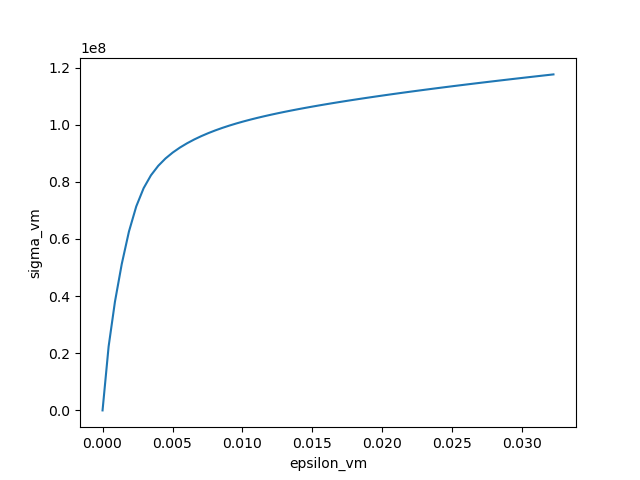
\includegraphics[width=0.5\textwidth]{images/plot.png}
    \caption{von Mises Equivalent stress-strain curve for pure Mg under shear.}
    \label{Benchmark_simulation}
\end{figure}


%\subsection{Comparison study with previous models.}
%Once the benchmark is chosen we apply it to test our model and we also use it to test our model with previous models.

%\subsubsection{Parametric studies on the model}
%In the final stage we carry out parametric studies of our model with experimental results.

\subsection{Comparison of Different Constitutive Models.}
It is essential to compare the computational efficiency and prediction capability of different constitutive models to assess their relative strengths and limitations. Since the MTech project spanning one year was dedicated to developing the constitutive model, comparative studies and analysis can be conducted as an extension of this work.

\subsection{Computational Efficiency.}
The computational effort required to generate the results can be compared across different models. For a fair comparison, the same inputs should be used to run the simulations, including the representative volume element, material parameters, and boundary conditions. Since the development of our model focused on computational efficiency, assessing its performance in this aspect will be a crucial future scope of this research work.

\subsection{Prediction capability.}
Our current model predicts the spatial evolution of twinning as a discrete quantity, which is physically accurate. In other words, our model predicts the texture evolution resulting from deformation twinning. It is also possible to compare other parameters, such as the load-deformation response, from different models and with experimental results to evaluate their predictive capabilities.

\subsection{Parametric Study of the model results.}
The influence of various parameters, including texture, grain size, grain morphology, strain rate, and loading conditions, on deformation twinning can be studied using the results of the model. These results can be compared with experimental data to validate the model's ability to capture the effects of different parameters accurately.

\subsection{Validation and Verification.}
It is crucial to validate and verify the constitutive model by comparing its predictions with experimental observations and established theoretical frameworks. This process involves assessing the model's ability to reproduce known phenomena accurately and ensuring that its underlying assumptions and formulations are consistent with fundamental principles.

\section{Future Scope: Implementation in ABAQUS as UMat.}
While DAMASK provides a basic finite element solver, a future implementation of the discrete twinning model can be made as a user-defined material (UMAT) in the ABAQUS finite element software. ABAQUS is a widely used and well-established commercial software package for finite element analysis, offering several advantages for the implementation and deployment of advanced constitutive models.




\subsection{ABAQUS Software:}
Robust and Stable Solvers: ABAQUS offers implicit finite element solvers renowned for their numerical stability and convergence properties, enabling the accurate simulation of complex material behavior and large deformations.

\begin{itemize}
    \item \textbf{User-Defined Material Capabilities:} ABAQUS allows users to implement custom constitutive models through UMATs, providing a flexible framework for incorporating advanced material models into simulations.
    \item \textbf{Pre- and Post-Processing Tools:} ABAQUS includes comprehensive pre-processing tools for model generation, mesh generation, and boundary condition assignment, as well as post-processing tools for visualizing and analyzing simulation results.
\end{itemize}

\subsection{Advantages of the Finite Element Method (FEM):}

\begin{itemize}
    \item \textbf{Complex Alloy System Modeling:} FEM can handle complex alloy systems where microstructural features such as precipitates, phases, and grains with complex morphologies can be accurately modeled into the Representative Volume Element (RVE) and discretized using tetrahedral or hexahedral elements.
    \item \textbf{Accurate Representation of Geometry and Boundary Conditions:} FEM allows for the precise representation of complex geometries and the application of a wide range of boundary conditions, enabling realistic simulations of actual engineering components and structures.
    \item \textbf{Adaptive Mesh Refinement:} Advanced FEM solvers like ABAQUS offer adaptive mesh refinement capabilities, which can automatically refine the mesh in regions of high deformation gradients or stress concentrations, improving the accuracy of the solution while optimizing computational resources.
\end{itemize}

\subsection{Additional Advantages: Wide Industry Adoption: }

ABAQUS is widely adopted across various industries, including automotive, aerospace, and manufacturing, ensuring compatibility with industry-standard practices and facilitating knowledge transfer and collaboration.


 %${https://petsc.org/release/overview/integrator_table/}$
 %$https://mooseframework.inl.gov/syntax/Executioner/TimeIntegrator/$
 % https://mooseframework.inl.gov/source/materials/crystal_plasticity/FiniteStrainUObasedCP.html
 % https://mooseframework.inl.gov/source/materials/crystal_plasticity/ComputeMultipleCrystalPlasticityStress.html
 % https://www.dropbox.com/s/23wj304q5rnjrtd/WARP3D_Intro_Lecture.pdf?e=1&dl=0

\appendix
\chapter{Continuum Mechanics.}
\label{Appendix:Continuum_mechanics}

\subsubsection{Continuum Description.}
Continuum description assumes a hypothetical continuous medium to describe behavior of a fluid/solid body. This allows description of material using continuous mathematical functions.

\subsubsection{Mechanics.}
Mechanics is classified into statics and dynamics. In crystal plasticity we study dynamics of plastic deformation. Dynamics can be further classified into Kinematics and Kinetics.

\begin{itemize}
    \item Kinematics: Study of deformation in the continuum element under consideration. Quantities measured are displacements, strains, velocities and strain rates.
    \item Kinetics: Study of forces and moments acting on the continuum object and how it affects displacements/strains or velocities/strain-rates. It involves description of material behaviour by quantification of traction/stresses and body forces using constitutive laws, material properties and conservation laws.
\end{itemize}

\section{Continuum Mechanics description of a body undergoing deformation.}

The figure \ref{Continuum_body_deformation} shows the undeformed continuum body $\mathcal{B}_0$ in reference configuration and deformed body $\mathcal{B}_t$ in current configuration. Reference configuration is time independent and current configuration is time dependent. If the deformation is described in reference/material configuration it is called Lagrangian description and if it is described in current/spatial configuration it is called Eulerian description.

Displacement at a given deformation state (at time = t) is given by,
\begin{equation}
\label{eq:A1}
    u(X) = x(X) - X
\end{equation}

A line segment $dX$ in reference configuration is transformed transformed to current configuration as,
\begin{equation}
\label{eq:A2}
    x(X) + dx = x(X) + \frac{\partial x}{\partial X}.\textrm{d}X + \textrm{O} (\textrm{d}X^2)
\end{equation}


\begin{figure}[H]
    \centering
    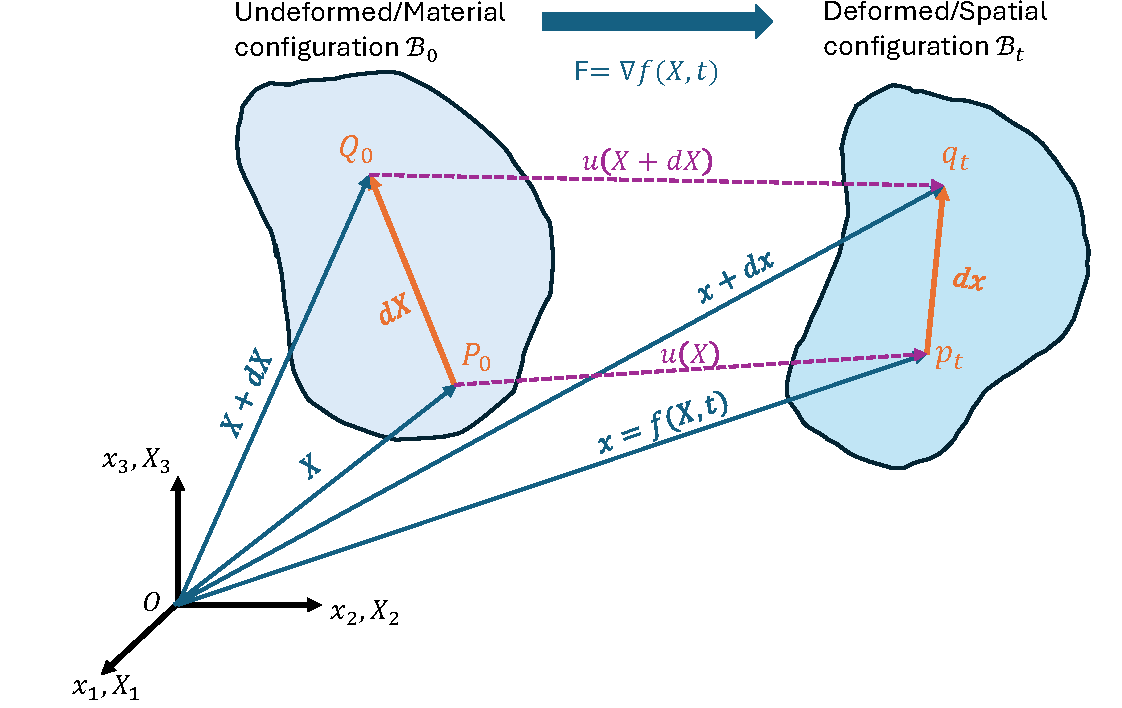
\includegraphics[width=0.9\textwidth]{images/Continuum_Mechanics_configurations.pdf}
    \caption{Deformation of a continuum body.}
    \label{Continuum_body_deformation}
\end{figure}

Neglecting higher order terms $\textrm{O} (\textrm{d}X^2)$,
\begin{equation}
\label{eq:A3}
    dx = \frac{\partial x}{\partial X}.\textrm{d}X = F.\textrm{d}X
\end{equation}

where $F:=\frac{\partial x}{\partial X}$ is called deformation gradient, a second order tensor. The deformation gradient maps the vector $\textrm{d}X$ at $X$ in the reference configuration to the vector $\textrm{d}x$ at $x$ in the current configuration. It is a 2-leg tensor because has one base at reference and one at current configuration.

From equations \ref{eq:A1} and \ref{eq:A3},
\begin{equation}
\label{eq:A4}
    F = \frac{\partial u + X}{\partial X}
\end{equation}

\begin{equation}
\label{eq:A5}
    F = I + \frac{\partial u}{\partial X}
\end{equation}

where $U:=\frac{\partial u}{\partial X}$ is called displacement gradient. Displacement gradient and deformation gradient are used to describe deformation of a body. Both are 2-leg tensors.

\section{Strain Measures}

It is possible to describe deformation only in the reference configuration as follows:

\begin{align*}
    \textrm{d}x.\textrm{d}x - \textrm{d}X.\textrm{d}X &= F.\textrm{d}X.F.\textrm{d}X -\textrm{d}X.\textrm{d}X \\
    &= \textrm{d}X.(F^T . F).\textrm{d}X - \textrm{d}X.\textrm{d}X \\
    &= \textrm{d}X.(F^T . F - I).\textrm{d}X \\
    &= \textrm{d}X.(2E_0).\textrm{d}X
\end{align*}
where $E_0 = \frac{1}{2}(F^T . F - I)$ is called Green-Lagrange strain tensor which is defined only in reference configuration.

Similarly, it is also possible to describe deformation in current configuration
\begin{align*}
    \textrm{d}x.\textrm{d}x - \textrm{d}X.\textrm{d}X &= \textrm{d}x.\textrm{d}x - F^{-1}.\textrm{d}x.F^{-1}.\textrm{d}x\\
    &= \textrm{d}x.\textrm{d}x - \textrm{d}x.(F^{-T} . F^{-1}).\textrm{d}x\\
    &= \textrm{d}x.(I - F^{-T} . F^{-1}).\textrm{d}x \\
    &= \textrm{d}X.(2E_t).\textrm{d}X
\end{align*}
this leads to definition of Euler-Almansi strain tensor $E_t = \frac{1}{2}(I - F^{-T} . F^{-1})$ which is defined only in current configuration.

Cauchy strain can be defined in terms of displacement gradient as,
\begin{equation}
    \epsilon = \frac{1}{2} \left( \nabla u + ( \nabla u)^T \right)
\end{equation}

For ONE-DIMENSION cases without lateral contraction the deformation can be described in terms of two variables: length in reference configuration $l_0$ and length in current configuration $l_t$ . By defining the ratio of these two variables as 'stretch ratio $\lambda$' we can compare the strain measures as given in the table \ref{Strain_measures_def}

\begin{table}[H]
    \centering
    \caption{Definition of strain measures for 1D cases}
    \begin{tabular}{c|cc}
        configuration & strain measure & definition in 1D \\
        \hline
        reference & Green-Lagrange strain & $E_{0,1dim = \frac{1}{2}(\lambda^2-1)}$ \\
        current & Euler-Almansi strain &  $E_{t,1dim = \frac{1}{2}(1 - \frac{1}{\lambda^2})}$ \\
        2-leg & Cauchy strain & $\epsilon_{1dim} = \lambda - 1$
    \end{tabular}
    
    \label{Strain_measures_def}
\end{table}

\section{Stress Measures}
Stress is a second order tensor defined using force and area vectors which can be defined in reference or current configuration. As a result different stress measures exist.

The stress measures along with strain measures are summarized in the table \ref{Stress_Measures_Configurations}. 

\begin{table}[H]
\centering
\caption{Stress and Strain measures in different configurations.}
\renewcommand\arraystretch{1.4}
\renewcommand\baselinestretch{1.4}
\begin{tabular}{c|ccc}
    configuration & stress & strain & symmetry \\
    \hline
    current/spatial & Cauchy Stress & Euler-Almansi strain & symmetric \\
    2-leg & 1st Piola-Kirchhoff stress & Displacement Gradient & non-symmetric\\
    reference/material & 2nd Piola-Kirchhoff stress & Green-Lagrange strain & symmetric\\
\end{tabular}

\label{Stress_Measures_Configurations}
\end{table}

The conversion between different stress measures used in DAMASK is given in table \ref{Stress_measures}

\begin{table}[H]
\centering
\caption{Conversion between different stress measures used in DAMASK.}
\renewcommand\arraystretch{1.4}
\renewcommand\baselinestretch{1.4}
\begin{tabular}{c|c|c|c}
    & $P$ (PK1)) & $S$ (PK2) & $\sigma$ (Cauchy) \\
    \hline
    $P$ & $P$ & det$F_pF_eF_iSF_p^{-T}$ & det$F\sigma F^{-T}$ \\
    $S$ & $\frac{1}{\mbox{det} F_p}F_i^{-1}F_e^{-1}PF_p^T$ & $S$ & det$(F_eF_i)F_i^{-1}F_e^{-1}\sigma F_e^{-T}F_i^{-T}$\\
    $\sigma$ & $\frac{1}{\mbox{det}F}PF^T$ & $\frac{1}{\mbox{det} (F_eF_i)}F_eF_iSF_i^{T}F_e^{T}$ & $\sigma$\\
\end{tabular}

\label{Stress_measures}
\end{table}

\section{Constitutive relation for Linear Elasticity}
Each stress components can be expressed as a linear combination of strain components in linear elasticity theory or Hooke's law, which is written as:
\begin{equation*}
    \sigma_{ij} = c_{ijkl} \epsilon_{kl}
\end{equation*}

where $c_{ijkl}$ are components of the elastic stiffness tensor. The symmetries in the strain and the stress reduce 81 different entries in the elastic tensor to 36 independent elements.
In the linear elasticity, the potential energy must be quadratic function of elastic strain. This further reduces the number of independent elements to 21.

Various crystallographic symmetries in the lattice structure reduces the number of independent elastic constants further as given in the table \ref{Independent_Cijkl}. To simplify representation of elastic constants Vogit notation is used in the below table where indices are mapped as: $11\to 1, \ 22 \to 2, \ 33 \to 3, \ 23\&32 \to 4, \ 13\&31 \to 4, \ 12\&21 \to 6$ 

\begin{table}[H]
\centering
\caption{Independent elastic constants for various crystal symmetries.}
\begin{tabular}{c m{4em} c}
    \hline
    Crystal Class & Independent $C_{ij}$ & List of independent $C_{ij}$ \\
    \hline
    Triclinic & 21 & All possible combinations \\
    Monoclinic & 13 & $C_{11}, C_{12}, C_{13}, C_{16}, C_{22}, C_{23}, C_{26}, C_{33}, C_{36}, C_{44}, C_{45}, C_{55}, C_{66}$ \\
    Orthorhombic & 9 & $C_{11}, C_{12}, C_{13}, C_{22}, C_{23}, C_{33}, C_{44}, C_{55}, C_{66}$ \\
    Trigonal & 6 or 7 & $C_{11}, C_{12}, C_{13}, C_{14}, C_{25},  C_{33}, C_{44}$ \\
    Tetragonal & 6 & $C_{11}, C_{12}, C_{13}, C_{33}, C_{44}, C_{66}$ \\
    Hexagonal & 5 & $C_{11}, C_{33}, C_{44}, C_{12}, C_{14}$ \\
    Cubic & 3 & $C_{11}, C_{12}, C_{44}$ \\
    Isotropic & 2 & $C_{11}, C_{44}$ \\
    \hline
\end{tabular}

\label{Independent_Cijkl}
\end{table}




\chapter{Implementation of correspondence matrix in DAMASK.}
\label{Appendix:Correspondence_matrix}
The correspondence matrix method allows predicting how crystallographic directions and planes transform during twinning. This approach is crucial for analyzing defects inherited from twinning, interactions between slip dislocations and twin boundaries, incorporating parent dislocations into the twinned lattice, and dealing with twin-twin intersections and double twinning. According to Niewczas \cite{Niewczas121}, most current continuum models for plastic deformation of crystals treat twinning incorrectly by only considering rotations, missing important aspects of the lattice transformation. Correspondence matrix approach (an example given in Table \ref{tab:Shear and correspondence matrices for Mg}) is implemented in DAMASK and utilized in the discrete twinning model.

\begin{table}[H]
\centering
\caption{Characteristic Shear and Correspondence matrices for different twinning modes of Mg with c/a=1.624.}
    \begin{tabular}{ccc}
    \hline
    $K_1 / \eta_1$ & Magnitude of shear $s$ & Correspondence matrix $C$ \\
    \hline
    $( \bar{1} 0 1 2 ) [1 0 \bar{1} 1] $ & 0.128917 &  $\begin{bmatrix}  -0.25 & 0.433 & -0.924 \\ 0.433 & -0.75 & -0.533 \\  -0.812 & -0.47 & 0 \end{bmatrix}$ \\
    $( 1 0 \bar{1} 1 ) [1 0 \bar{1} \bar{2}] $ & 0.137717 & $\begin{bmatrix}  0.125 & 0.65 & 0.693 \\ 0.65 & -0.625 & 0.4 \\  0.812 & 0.47 & -0.5 \end{bmatrix}$ \\
    $( 1 0 \bar{2} \bar{2} ) [1 1 \bar{2} \bar{3}] $ & 0.261649 & $\begin{bmatrix}  -0.67 & 0.577 & 0.411 \\ 0.577 & 0 & 0.711 \\  0.54 & 0.937 & -0.333 \end{bmatrix}$ \\
    $( 1 1 \bar{2} 1) [\bar{1}\bar{1} 2 6] $ & 0.615764 & $\begin{bmatrix}  -0.5 & 0.866 & 0.308 \\ 0.866 & 0.5 & 0.533 \\  0.0 & 0.0 & -1.0 \end{bmatrix}$ \\
    \hline
    \end{tabular}

\label{tab:Shear and correspondence matrices for Mg}
\end{table}


\begin{minted}[fontsize=\scriptsize, frame=single]{fortran}

module math

implicit none

contains

function math_axisAngleToR(axis,omega) result(math_axisAngleToR1)
!------------------------------------------------
!> Function to generate rotation matrix around 
!> arbitrary direction and arbitrary angle
!------------------------------------------------

  implicit none
  
  real, dimension(3), intent(in) :: axis
  real, intent(in) :: omega
  real, dimension(3) :: n
  real :: norm,s,c,c1
  
  real, dimension(3,3), parameter :: &
  I3 = real(reshape([&
    1, 0, 0, &
    0, 1, 0, &
    0, 0, 1  &
    ],shape(I3)))       !< 3x3 Identity

  real, dimension(3,3) :: math_axisAngleToR1
  
  norm = norm2(axis)
  wellDefined: if (norm > 1.0e-8) then
    n = axis/norm       ! normalize axis to be sure
  
    s = sin(omega)
    c = cos(omega)
    c1 = 1.0 - c
  
    math_axisAngleToR1(1,1) =  c + c1*n(1)**2.0
    math_axisAngleToR1(1,2) =  c1*n(1)*n(2) - s*n(3)
    math_axisAngleToR1(1,3) =  c1*n(1)*n(3) + s*n(2)
                              
    math_axisAngleToR1(2,1) =  c1*n(1)*n(2) + s*n(3)
    math_axisAngleToR1(2,2) =  c + c1*n(2)**2.0
    math_axisAngleToR1(2,3) =  c1*n(2)*n(3) - s*n(1)
                              
    math_axisAngleToR1(3,1) =  c1*n(1)*n(3) - s*n(2)
    math_axisAngleToR1(3,2) =  c1*n(2)*n(3) + s*n(1)
    math_axisAngleToR1(3,3) =  c + c1*n(3)**2.0
  else wellDefined
    math_axisAngleToR1 = I3
  endif wellDefined
  
end function

end module math


program corresponcence_matrix
use math
implicit none

integer, dimension(4) :: &
    active = [6,6,6,6], &  !< number of active twin systems
    potential = [6,6,6,6]  !< all the potential twin systems

real, dimension(3) :: &
    direction, normal

real, dimension(3,24) :: normal_vector, direction_vector

real, dimension(3,3,24) :: SchmidMatrix, corresponcenceMatrix

real, dimension(24) :: characteristicShear

real :: cOverA = 1.6235

real :: pi = 3.14159274 

real, dimension(8,24) :: &
system = reshape(real([&
! <-10.1>{10.2} systems, shear = (3-(c/a)^2)/(sqrt(3) c/a)
! tension in Co, Mg, Zr, Ti, and Be; compression in Cd and Zn
     -1,  0,  1,  1,     1,  0, -1,  2, & !
     0, -1,  1,  1,     0,  1, -1,  2, &
     1, -1,  0,  1,    -1,  1,  0,  2, &
     1,  0, -1,  1,    -1,  0,  1,  2, &
     0,  1, -1,  1,     0, -1,  1,  2, &
    -1,  1,  0,  1,     1, -1,  0,  2, &
! <11.6>{-1-1.1} systems, shear = 1/(c/a)
! tension in Co, Re, and Zr
    -1, -1,  2,  6,     1,  1, -2,  1, &
     1, -2,  1,  6,    -1,  2, -1,  1, &
     2, -1, -1,  6,    -2,  1,  1,  1, &
     1,  1, -2,  6,    -1, -1,  2,  1, &
    -1,  2, -1,  6,     1, -2,  1,  1, &
    -2,  1,  1,  6,     2, -1, -1,  1, &
! <10.-2>{10.1} systems, shear = (4(c/a)^2-9)/(4 sqrt(3) c/a)
! compression in Mg
    1,  0, -1, -2,     1,  0, -1,  1, &
     0,  1, -1, -2,     0,  1, -1,  1, &
    -1,  1,  0, -2,    -1,  1,  0,  1, &
    -1,  0,  1, -2,    -1,  0,  1,  1, &
     0, -1,  1, -2,     0, -1,  1,  1, &
     1, -1,  0, -2,     1, -1,  0,  1, &
! <11.-3>{11.2} systems, shear = 2((c/a)^2-2)/(3 c/a)
! compression in Ti and Zr
    1,  1, -2, -3,     1,  1, -2,  2, &
    -1,  2, -1, -3,    -1,  2, -1,  2, &
    -2,  1,  1, -3,    -2,  1,  1,  2, &
    -1, -1,  2, -3,    -1, -1,  2,  2, &
    1, -2,  1, -3,     1, -2,  1,  2, &
    2, -1, -1, -3,     2, -1, -1,  2  &
    ]),shape(system))

real, dimension(3,3), parameter :: &
I3 = real(reshape([&
    1, 0, 0, &
    0, 1, 0, &
    0, 0, 1  &
    ],shape(I3)))  !< 3x3 Identity

integer :: &
    a, &                 !< index of active system
    p, &                 !< index in potential system matrix
    f, &                 !< index of my family
    s, &                 !< index of my system in current family
    f1, s1, e1, i, j, k  !< indices for similar loops


!-----------------------------------------------------------
!> Normal vector to twin plane and direction vector 
!> of the twin
!-----------------------------------------------------------
    
a = 0
do f = 1, size(active,1)         !< Active Twin Modes
    do s = 1, active(f)          !< Active twin systems
            
        a = a + 1
        p = sum(potential(1:f-1))+s                                         
! direction [uvtw]->[3u/2 (u+2v)*sqrt(3)/2 w*(p/a)])       
        direction = [ system(1,p)*1.5, &
        (system(1,p)+2.0*system(2,p))*sqrt(0.75), &
         system(4,p)*cOverA ]
            
! plane (hkil)->(h (h+2k)/sqrt(3) l/(p/a))
        normal    = [ system(5,p), &
        (system(5,p)+2.0*system(6,p))/sqrt(3.0), &
        system(8,p)/cOverA ]                                              
        normal_vector(1:3,a) = normal /norm2(normal)
        direction_vector(1:3,a) = direction / norm2(direction)
            
    end do
end do

!-----------------------------------------------------------
!> Magnitude of Characteristic shear for twinning modes 
!-----------------------------------------------------------

do f1 = 1,size(active,1)       !< Active twin modes
    s1 = sum(active(:f1-1)) + 1
    e1 = sum(active(:f1))
    select case(f1)
    case (1)
    characteristicShear(s1:e1) = (3.0-cOverA**2)/sqrt(3.0)/cOverA
    case (2)
    characteristicShear(s1:e1) = 1.0/cOverA
    case (3)
    characteristicShear(s1:e1) = (4.0*cOverA**2-9.0)/sqrt(48.0)/cOverA
    case (4)
    characteristicShear(s1:e1) = 2.0*(cOverA**2-2.0)/3.0/cOverA
      end select
enddo
    
!> Write results for characteristic shear

write(6,*)'characteristic shear, for [1,  0, -1,  1],(-1,  0,  1,  2)'
write(6,*)characteristicShear(4)
write(6,*)'characteristic shear, for [-1, -1,  2,  6],(1,  1, -2,  1)'
write(6,*)characteristicShear(7)
write(6,*)'characteristic shear, for [1,  0, -1, -2],(1,  0, -1,  1)'
write(6,*)characteristicShear(13)
write(6,*)'characteristic shear, for [1,  1, -2, -3],(1,  1, -2,  2)'
write(6,*)characteristicShear(19)
    
!---------------------------------------------------------------
!> SchmidMatrix = Outer product of direction and normal vectors.
!---------------------------------------------------------------

do i = 1, sum(active)
    forall(j=1:3, k=1:3) &
    SchmidMatrix(j,k,i) = direction_vector(j,i) * &
                           normal_vector(k,i)
enddo

!--------------------------------------------------------------
!> Correspondence Matrix = Reorientation * Shear
!--------------------------------------------------------------

do i = 1, sum(active)
    corresponcenceMatrix(1:3,1:3,i) = matmul(math_axisAngleToR &
                                      (normal_vector(1:3,i),pi),&
                                      I3+characteristicShear(i) &
                                      *SchmidMatrix(1:3,1:3,i))
enddo

!> Write results for Correspondence Matrix
    
write(6,*)'correspondence matrix for [1,  0, -1,  1],(-1,  0,  1,  2)'
write(6,*)corresponcenceMatrix(1:3,1:3,4)
write(6,*)'oxoxoxoxoxoxoxoxoxoxoxoxoxoxoxoxoxoxoxoxoxoxoxox'
write(6,*)'correspondence matrix for [-1, -1,  2,  6],(1,  1, -2,  1)'
write(6,*)corresponcenceMatrix(1:3,1:3,7)
write(6,*)'oxoxoxoxoxoxoxoxoxoxoxoxoxoxoxoxoxoxoxoxoxoxoxox'
write(6,*)'correspondence matrix for [1,  0, -1, -2],(1,  0, -1,  1)'
write(6,*)corresponcenceMatrix(1:3,1:3,13)
write(6,*)'oxoxoxoxoxoxoxoxoxoxoxoxoxoxoxoxoxoxoxoxoxoxoxox'
write(6,*)'correspondence matrix for [1,  1, -2, -3],(1,  1, -2,  2)'
write(6,*)corresponcenceMatrix(1:3,1:3,19)


end program corresponcence_matrix


\end{minted}

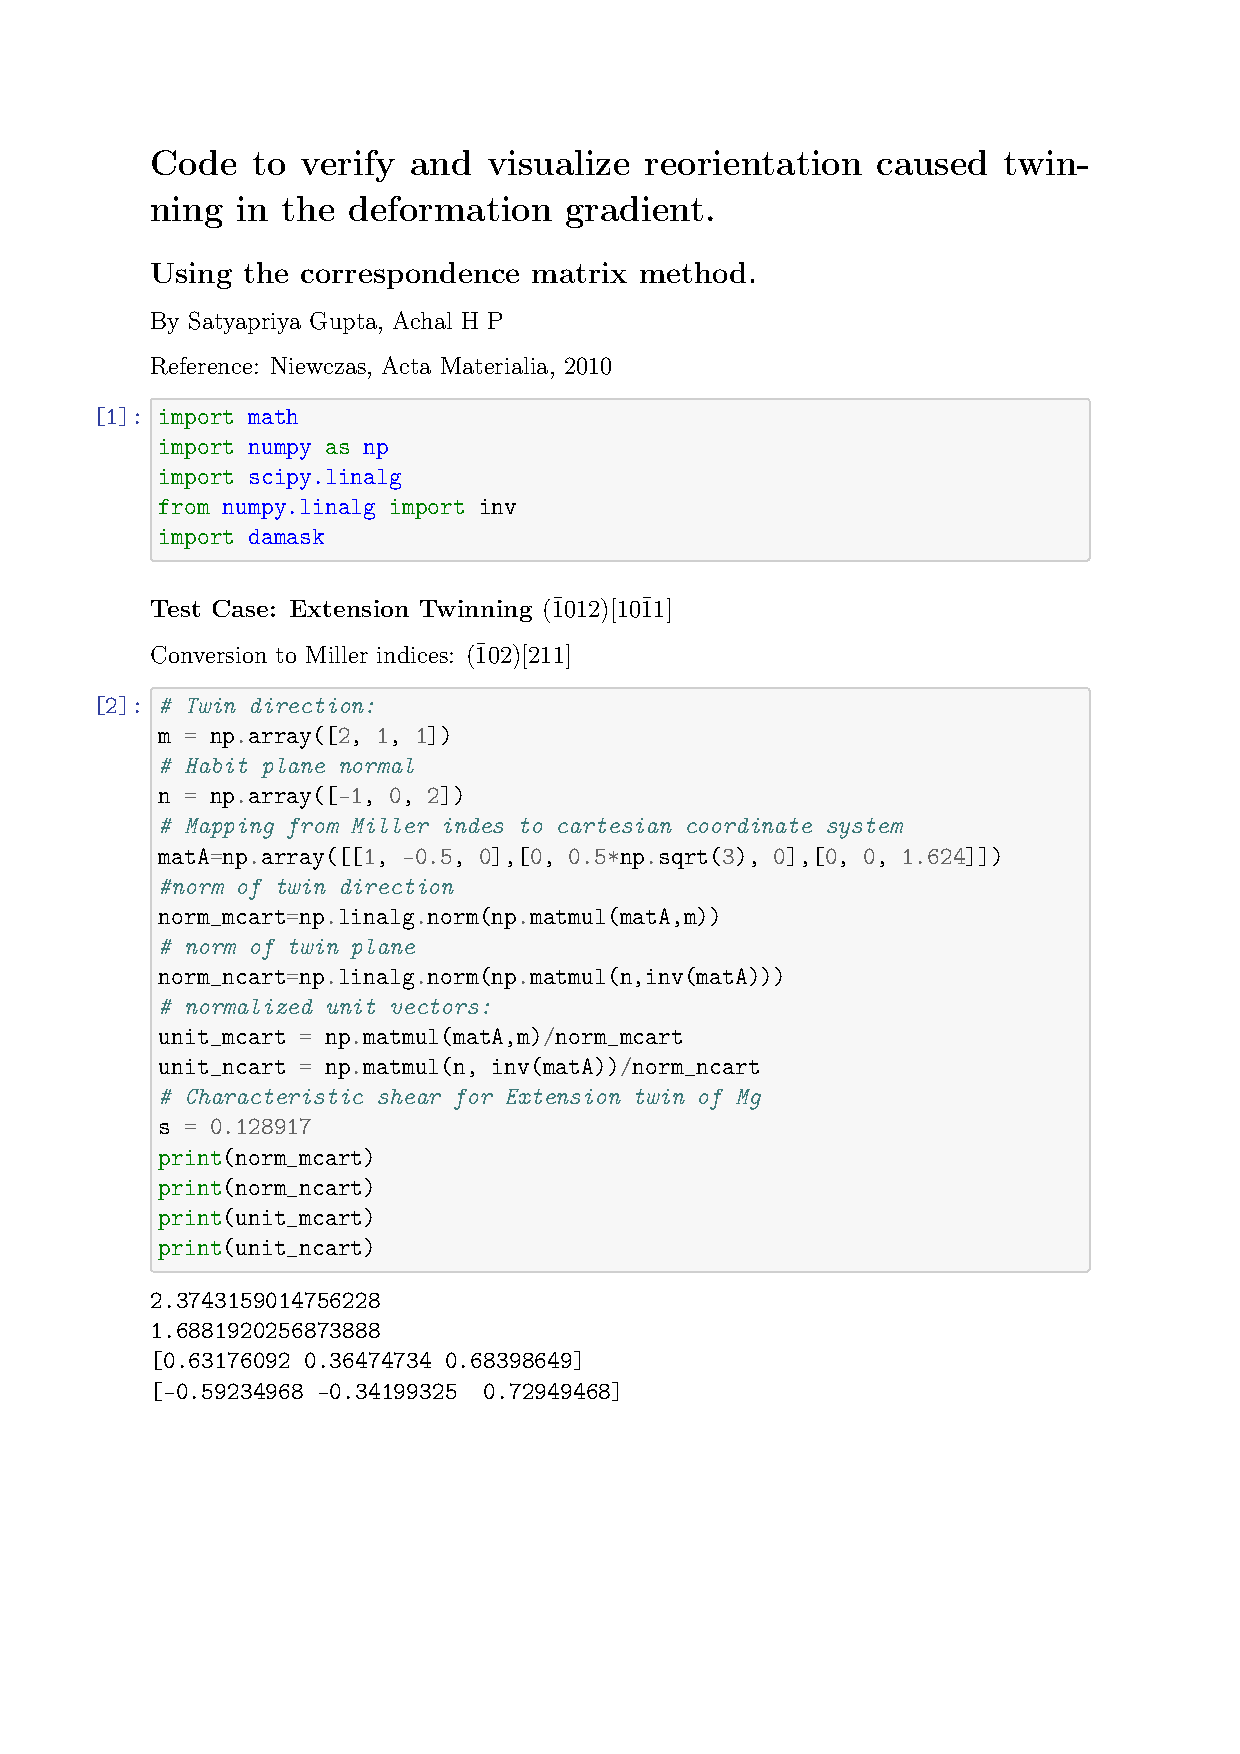
\includepdf[pages=-, addtotoc={2, chapter, 2, Code to verify and visualize reorientation by twinning, lbl:pdfsection}, pagecommand={\thispagestyle{plain}}, offset=10mm -28mm]{Code_to_check_reorientation.pdf}

\chapter{DAMASK Source Code Installation.}
\label{Appendix:DAMASK_source_code_compilation}
Source code compilation of DAMASK was required for our work because it involved modifying the source code.
\section{Install Dependencies}
DAMASK uses many open source libraries which has to be installed before installing it. DAMASK developers have provided bash script which gives an overview of the prerequisites available in the computer.

\begin{lstlisting}[language=bash, basicstyle=\small\ttfamily, frame=single]
wget https://damask.mpie.de/files/installation/3.0.0-
beta/DAMASK_prerequisites.sh
sh ./DAMASK_prerequisites.sh
cat system_report.txt
\end{lstlisting}

Running the below bash script as superuser will install all the DAMASK dependencies.

\begin{lstlisting}[language=bash, basicstyle=\small\ttfamily, frame=single]

#!/bin/bash

# Script to install DAMASK dependencies and PETSc in home 
# directory
# References: Researchgate & https://damask.mpie.de/

#Go to home directory
cd "$HOME" || exit

#install dependencies
sudo apt install git build-essential cmake make autoconf 
mpich libopenmpi-dev bison cmake-format liblapack-dev 
libblas-dev python3 python3-pip python3-setuptools python3-vtk9 
python3-numpy python3-scipy python3-pandas python3-matplotlib 
python3-h5py

# Download PETSc source and pick the version
git clone https://gitlab.com/petsc/petsc.git
cd petsc/
git checkout v3.15.5

# Configure PETSc
./configure --with-cc=mpicc --with-cxx=mpicxx --with-fc=mpif90
--download-fblaslapack --download-hdf5 --download-fftw 
--download-superlu --download-hypre --download-mumps 
--download-ml --download-scalapack --with-hdf5-fortran-bindings 
--download-chaco --download-netcdf --download-exodusii 
--download-metis --download-parmetis --download-suitesparse 
--download-superlu --download-superlu_dist  --download-triangle 
--with-c2html=0  --with-debugging=0 --with-ssl=0 --with-x=0 
--download-zlib --download-cmake --download-pnetcdf 
--with-cxx-dialect=C++11 COPTFLAGS="-O3 -march=native" 
CXXOPTFLAGS="-O3 -march=native" FOPTFLAGS="-O3 -march=native"
 PETSC_ARCH=gfortran -PETSC_DIR=`pwd` --with-debugging=0

#Build
make PETSC_DIR=$HOME/petsc PETSC_ARCH=gfortran all
#Check
make PETSC_DIR=$HOME/petsc PETSC_ARCH=gfortran check

#Go to home directory
cd "$HOME" || exit

# Lines to be added to .bashrc
lines=($'export PETSC_DIR=/home/achal/petsc\nexport
PETSC_ARCH=gfortran\nexport XAUTHORITY=~/.Xauthority\nexport
HWLOC_COMPONENTS=-gl')

# Check if .bashrc exists
if [ -f ~/.bashrc ]; then
    # Append the lines to the end of .bashrc
    printf "%s\n" "${lines[@]}" >> ~/.bashrc
    echo "Lines appended to ~/.bashrc"
else
    echo "Error: ~/.bashrc does not exist"
    exit 1
fi

echo "Dependencies installed."
echo "================================"
echo -e "Run command: 'source .bashrc'"

\end{lstlisting}

\subsection{Git}
Git is a distributed version control system for tracking changes in source code during software development. It was created in 2005 by Linus Torvalds, the principal developer of the Linux kernel.
\subsection{GNU compiler Collection.}
The GNU Compiler Collection is a open source project which provides set of compilers for various programming languages including C, C++, Fortran, and others. It was developed by the GNU Project, a free software project of the Free Software Foundation (FSF).
\subsection{CMake}
CMake is a cross-platform tool that helps build, test, and package software by generating native makefiles and project files. It allows developers to write portable configuration files that can build their software across different platforms and compilers.
\subsection{MPI}
Message Passing Interface (MPI) is a standardized and portable message-passing system designed for distributed and parallel computing. It allows multiple computers (or even multiple processor cores within the same computer) to exchange messages across distributed memory.
\subsection{PETSc}
Portable, Extensible Toolkit for Scientific Computation (PETSc) is a large library of simulation software developed by Argonne National Laboratory \cite{balay2020petsc}. It contains parallel linear and nonlinear equation solvers, ODE integrators, and optimization algorithms.

\section{Run Checks and Install DAMASK}
PETSc setup can be checked using an example that can be downloaded from DAMASK website:

\begin{lstlisting}[language=bash, basicstyle=\small\ttfamily, frame=single]
wget https://damask.mpie.de/files/installation/3.0.0-beta/
PETSc_test.tar.xz

tar -xf PETSc_test.tar.xz
cd PETSc_test
make PETSc_test
mpirun -np 2 ./PETSc_test
\end{lstlisting}

Downloading, compilation and installation of DAMASK can be done using the bash script below:

\begin{lstlisting}[language=bash, basicstyle=\small\ttfamily, frame=single]
#!/bin/bash

# Source: https://damask.mpie.de/release/installation/
source_code.html

# Create the DAMASK directory
mkdir DAMASK
cd DAMASK

# Download and extract DAMASK
wget https://damask.mpie.de/download/damask-3.0.0-beta.tar.xz
wget https://damask.mpie.de/download/
damask-3.0.0-beta.tar.xz.sha256
sha256sum -c damask-3.0.0-beta.tar.xz.sha256 && tar -xf 
damask-3.0.0-beta.tar.xz

# Run cmake commands for grid solver
cmake -S damask-3.0.0-beta -B build-grid -DDAMASK_SOLVER=grid
cmake --build build-grid --target install

# Run cmake commands for mesh solver
cmake -S damask-3.0.0-beta -B build-mesh -DDAMASK_SOLVER=mesh
cmake --build build-mesh --target install

echo "Installed DAMASK_grid and DAMASK_mesh"
\end{lstlisting}

\bibliographystyle{IEEEtran}
\bibliography{references}

\end{document}
